%\documentclass[a4paper]{article}
\documentclass[a4paper,oneside]{memoir}
\usepackage[hscale=0.76,vscale=0.76]{geometry}
\setlength{\parindent}{0.0cm}
\setlength{\parskip}{1.4ex}
\usepackage{graphicx}
\usepackage{proof}
\usepackage{fancyvrb}
%%% Japanese
\usepackage{fontspec,xltxtra,xunicode}
\usepackage{indentfirst}

% freely available M+ fonts
\setmainfont[Mapping=tex-text]{M+ 2p regular}
\setsansfont[Mapping=tex-text]{M+ 2c regular}
\setmonofont[Mapping=tex-text]{M+ 2m medium}
%\setmainfont[Mapping=tex-text]{メイリオ}
%\setsansfont[Mapping=tex-text]{Hiragino Kaku Gothic ProN W3}
%\setmonofont[Mapping=tex-text]{Osaka-Mono}
%\setjamonofont{Osaka-Mono}
\XeTeXlinebreaklocale "ja"
\XeTeXlinebreakskip=0em plus 0.1em minus 0.01em
\XeTeXlinebreakpenalty=0
\renewcommand{\baselinestretch}{1.4}
\settowidth{\parindent}{あ}
%%%%
\usepackage{dcolumn,hhline,colortbl}
\usepackage[table]{xcolor}
%%%%% 色付表
\newcolumntype{G}{%
  >{\columncolor[gray]{0.9}}c}
\newcolumntype{O}{%
  >{\columncolor{orange}}c}
\newcolumntype{M}{%
  >{\columncolor{green}}c}
\newcolumntype{Y}{%
  >{\columncolor{yellow}}c}
\newcolumntype{C}{%
  >{\columncolor{cyan}}c}
%%%% hyperref
%\usepackage[dvipdfm,colorlinks=true,linkcolor=blue]{hyperref} 
\usepackage[colorlinks=true,linkcolor=blue]{hyperref} 
%%%% numbering
%%% ToC down to susubsections
\settocdepth{subsubsection}
%%% Numbering down to sections
\setsecnumdepth{subsection}
%%% 名前定義を適当に
\def\figurename{{図}}
\def\tablename{表}
\def\contentsname{目次}
\def\listfigurename{図目次}
\def\listtablename{表目次}
\def\refname{参考文献}
\def\bibname{参考文献}
\def\indexname{索引}
\def\appendixname{付録}
%%%%%%%%%% Verbatim
\DefineVerbatimEnvironment%
{simplev}{Verbatim}
{fontsize=\small}
\DefineVerbatimEnvironment%
{examplev}{Verbatim}
{frame=leftline,fontsize=\small}
%%%%%%%%%%
\definecolor{shadecolor}{gray}{0.9}
\newenvironment{vvtm}%
{\parskip=0pt\lineskip=0pt\begin{center}\begin{minipage}{0.8\textwidth}\begin{snugshade}}%
  {\end{snugshade}\end{minipage}\end{center}}
%\includeonly{appendix}
%%%%%%%%%%
\begin{document}
\headstyles{default}
\tightlists
\midsloppy
\raggedbottom
\chapterstyle{ell}
%%%%%%%%
\frontmatter
\pagestyle{empty}
% 表紙 %%%%%%%%%%%%%%%%%%%%%%%%%%%%%%%%%%%%%%%%%%%%%%%%%%%%%
\title{\textbf{PigNose 使用手引}\\ver 1.0 \\ --\textit{Draft}--}
\author{澤田 寿実\\
  info@cafeobj.org}
\date{}
\maketitle
  \begin{center}
    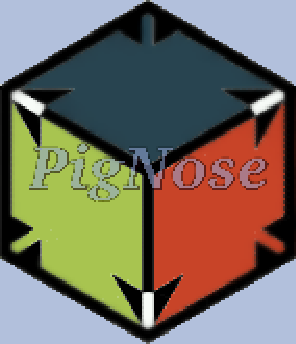
\includegraphics[scale=0.5]{pignose.pdf}
  \end{center}
\thispagestyle{empty}
\newpage
% 構成 %%%%%%%%%%%%%%%%%%%%%%%%%%%%%%%%%%%%%%%%%%%%%%%%%%%%%
\section*{はじめに}
本書は, CafeOBJ 言語で書かれた仕様のための自動定理証明システム
PigNose の利用手引である. 
システムは SRA版 CafeOBJ インタプリタ\footnote{今の所, CafeOBJ 言語のイ
  ンタプリタはこれしか存在しない. システムの入手先については第
  ~\ref{sec:distribution}節を参照されたい.} 
を拡張したものになっている. 
従って, これを用いるには CafeOBJ インタプリタの使用法
についても知っておく必要がある. 本書では, PigNose 特有のコマンドについて
のみ説明するので, 必要に応じて CafeOBJ インタプリタのマニュアル\footnote{CafeOBJ インタプリタのマニュアルは
   \url{http://cafeobj.org/download/} からダウンロード
   出来る}. 
を参照されたい.
また, ここでは CafeOBJ 言語についての説明も行わない. 本書では, CafeOBJ
言語については既知のものと仮定している. CafeOBJ 言語についての解説は, 文
献\cite{CafeRep}を参照して頂きたい. 
% PigNose は resolution 原理を用いた反駁法によって定理証明を行うシステムで
% あるが, これについての解説も行わない. 
% 必要に応じて, 参考文献 \cite{chang-lee} 等を参照して頂きたい.  

% \section*{本書の構成}

本文は4部構成でPigNoseシステムの使用法が説明されている.
第I部でシステムのインストール法を述べ, 第II部で反駁エンジン,
第III部で詳細化検証, 第IV部で安全性モデル検査について説明する.

\section*{バグレポート/提案}

システムの不具合に関する報告や, 改善提案等に関する
連絡は, 電子メイルで \texttt{info@cafeobj.org} まで頂きたい.

\newpage
% 目次 %%%%%%%%%%%%%%%%%%%%%%%%%%%%%%%%%%%%%%%%%%%%%%%%%%%%%
% \doparttoc
\tableofcontents
\newpage
%\listoffigures
%\newpage
\pagenumbering{arabic}
\mainmatter
% 本文 %%%%%%%%%%%%%%%%%%%%%%%%%%%%%%%%%%%%%%%%%%%%%%%%%%%%%
\part{$B%7%9%F%`35MW(B}
$B3+J|7?J,;64D6-$G$NItIJ$d%5!<%S%9$OJ,;6%*%V%8%'%/%H$H$7$FB*$($k$3$H$,(B
$B=PMh$k(B. $B$=$N5!G=(B/$BF0:n$NI=8=$K$OF~=PNO$N%G!<%?(B($B7?(B)$B$*$h$S(B, 
$BF0E*$J?6$kIq$$(B($B>uBVA+0\(B)$B$N5-=R$,I,MW$H$J$k(B.
$B$3$N>l9g(B, $B%$%s%?%U%'!<%9$NI=8=$K$O(B, 
$B8=:_0lHLE*$K9-$/;HMQ$5$l$F$$$k(B
IDL$B$N%Y!<%9$H$J$C$F$$$k35G0(B, $BI8<((B($B%7%0%K%A%c(B)$B$,M-8z$G$"$k(B.
$BF0:n$K4X$7$F$O(B, $B$=$l$,$&$^$/I=8=$G$-$k$@$1$G$O$J$/(B, 
$B8!>Z$r9T$&I,MW$,$"$k$3$H$+$i(B, $B$J$s$i$+$N7A<0E*$JO@M}BN7O$,I,MW$G$"$j(B,
$B$7$+$b(B, $B8zN(NI$/7W;;5!>e$G7A<0E*>ZL@$,<B9T=PMh$k$h$&$J$b$N$G$J$1$l$P(B
$B$J$i$J$$(B. 

$B>e$N$h$&$JMW7o$rDs6!$9$kOHAH$H$7$F(B, $B0lHL$K?6$kIq$$O@M}$HAm>N$5$l$k(B
$B7A<0I=8=$,E,@Z$G$"$k(B. 
$BItIJ$d%5!<%S%9$N;EMM$N5-=R$K$O$3$N$h$&$JO@M}E*OHAH$rDs6!$9$k7A<0;EMM8@8l$r(B
$BMQ$$$k$N$,NI$$(B.
$B$3$N$h$&$J8@8l$N0l$D$K!$1#JCBe?t$K4p$E$/?6$kIq$$;EMM$N5-=R$r2DG=$H$7$F$$$k(B 
CafeOBJ $B$,$"$k(B. 
CafeOBJ $B$OC1$K%*%V%8%'%/%H$N?6$kIq$$$N5-=R$K$H$I$^$i$:(B,
$B6/NO$J%G!<%?7?Dj5A$N5!G=(B, $B$^$?9bEY$J;EMM$N%b%8%e!<%k2=5!G=$r(B
$BHw$($F$$$k$?$aI=8=G=NO$KM%$l(B, $B4{B8$N(B IDL $B$J$I$K$h$k5-=R$r(B, $BMF0W$K(B
$B%^%C%T%s%0$9$k$3$H$,2DG=$G$"$k(B. $B$^$?(B, $B<BF/$9$k=hM}7O$,%U%j!<$G(B
$BF~<j$G$-$k(B. $B$3$N$3$H$+$i(B, $B8!>Z?dO@%7%9%F%`$O(B, CafeOBJ $B$N=hM}7O(B($B%$%s%?%W%j%?(B)
$B$r3HD%$7(B, $B$=$l$HM;9g$5$l$?%7%9%F%`$H$J$C$F$$$k(B.

$BItIJ$N8!:w!&8!>Z$r9T$&>e$G4pK\E*$H$J$k$N$,!$(B
\begin{enumerate}
\item[(1)] $B%7%0%K%A%c!&%^%C%A%s%0(B --- $B;EMM$N9=J8E*8!:w(B
\item[(2)] $B;EMM$N?6Iq>\:Y2=8!>Z(B
\item[(3)] $B?6Iq%b%G%k8!::K!$rMQ$$$?E}9g%7%9%F%`8!::(B
\end{enumerate}
$B$G$"$k!%(B
$BK\=q$GF3F~J}K!$*$h$S;HMQ<j0z$r@bL@$9$k(B\textbf{$B8!>Z?dO@%7%9%F%`(B}$B$O!$$3$l$i$N(B
$B4pK\MWAG$H$J$k5!G=$r(B CafeOBJ $B%$%s%?%W%j%?$r3HD%$9$k$3$H$GDs6!$7$?$b$N$G$"$k!%(B
$B>e$N(B (1) $B$H(B (2) $B$N5!G=$O!$J;$;$F(B \textbf{$B;EMM8!>Z%7%9%F%`(B} $B$H$7$F(B
$B9=@.$5$l$k!%(B(3) $B$N5!G=$O(B \textbf{$B%b%G%k8!::%7%9%F%`(B} $B$,Ds6!$9$k!%(B
$B$3$l$i(B2$B$D$N%7%9%F%`$N3K$H$7$F!$(B\textbf{$BH?G}%7%9%F%`(B} $B$,$"$k!%(B
$B;EMM8!>Z$*$h$S%b%G%k8!::$NN><T$H$b!$4pK\E*$K$ODjM}>ZL@$r9T$&$b$N$G$"$k!%(B
$B$3$N%7%9%F%`$G$O1#JCBe?t$r07$&$?$a!$>uBV6u4V$NA+0\$K4X$7$F$N>ZL@$,(B
$B9T$o$J$1$l$P$J$i$J$$!%$=$N$?$a!$>uBV6u4V$r=R8lO@M}$GI=8=$9$kJ}K!$r$H$j!$(B
$B$7$?$,$C$FDjM}>ZL@$O!$(B($BEy9fIU$-$N(B)$BB?%=!<%H0l3,=R8lO@M}$K$*$1$kDjM}>ZL@$H$J$k!%(B
$BH?G}%7%9%F%`$O!$$3$N$?$a$NDjM}>ZL@7O$G$"$j!$%7%9%F%`$NCf?4$OH?G}%7%9%F%`(B
$B$NDs6!$9$k!$(Bresolution $B$K4p$E$$$?H?G}%(%s%8%s$G$"$k!%(B
$B?^(B~\ref{fig:bigpink-arch} $B$K%7%9%F%`$N9=@.$r<($9!%(B

{\sloppy
\begin{figure}[htb]
  \begin{center}
%    \epsfxsize=0.8\textwidth
    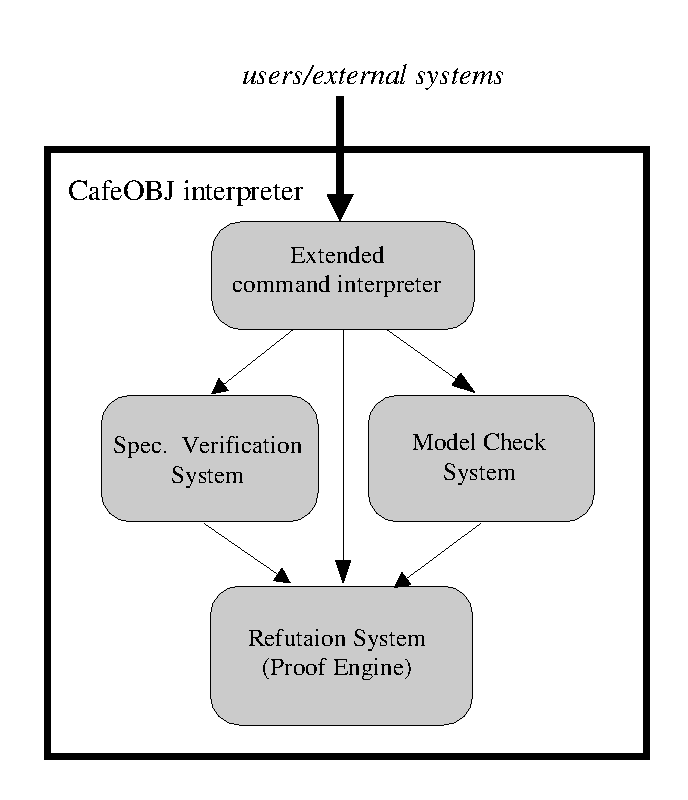
\includegraphics{bigpink-arch.eps}
    \caption{$B8!>Z?dO@%7%9%F%`$N9=@.(B}
    \label{fig:bigpink-arch}
  \end{center}
\end{figure}
}

$B?^(B~\ref{fig:bigpink-arch} $B$G(B, \textbf{Refinement Check System} $B$H$"$k$N$,(B
$B;EMM8!>Z%7%9%F%`(B, \textbf{Model Check System} $B$H$"$k$N$,(B $B%b%G%k8!::%7%9%F%`(B,
$B$^$?(B, \textbf{Refutation System} $B$H$J$C$F$$$k$N$,(B, $BH?G}%7%9%F%`$G$"$k(B.
$B$3$l$i$N%7%9%F%`$N5!G=$O(B, ($B3HD%$5$l$?(B) CafeOBJ $B%$%s%?%W%j%?$X$N%3%^%s%I(B
$B$H$7$F30It$XDs6!$5$l$k(B. $B$7$?$,$C$F(B, CafeOBJ $B$N%3%^%s%I%$%s%?%W%j%?$,(B
$B?75,$N%3%^%s%I$"$k$$$O9=J8$K$h$C$F3HD%$5$l$k(B. $B?^$G(B \textbf{Extended Command
Interpreter} $B$H$"$k$N$,(B, $B$3$N3HD%$5$l$?%3%^%s%I%$%s%?%W%j%?$G$"$k(B.
$B30It$NMxMQ<T$d%7%9%F%`$O(B, $B$3$N%3%^%s%I%$%s%?%W%j%?$rDL$8$F$3$l$i$N%7%9%F%`$N(B
$B5!G=$rMxMQ$9$k$3$H$K$J$k(B.

\section{$B;EMM8!>Z%7%9%F%`$N35MW(B}
\label{sec:refine-check-abstract}

$B;EMM8!>Z%7%9%F%`$O!$$"$kItIJ$N;EMM$,M?$($i$l$?;~$K!$$=$l$,MW5a;EMM$r(B
$BK~B-$9$k$b$N$+$I$&$+$r7A<0E*$K8!>Z$9$k$b$N$G$"$k!%(B

$B%7%9%F%`A4BN$NJ8L.$G8@$&$H!$(B
$B:G=i$O!$MW5a;EMM(B $R$ $B$H9gCW$9$k$h$&$JItIJ$N;EMM(B $P$ $B$r(B
$BC5:w$9$k$3$H$+$i;O$^$k!%$3$N;~$K%7%0%K%A%c%^%C%A%s%0$rMxMQ$7$F!$(B
$BMW5a;EMM$K9=J8E*$K9gCW$7$J$$$h$&$JItIJ;EMM$r$U$k$$$K3]$1$FJ'$$Mn$9$3$H$,=PMh$k!%(B
$B%7%0%K%A%c%^%C%A%s%0$O!$%^%C%A%s%0$,@.8y$9$k$H!$(B
$R$ $B$+$i(B $P$ $B$X$N;EMM<M(B $M$ (CafeOBJ$B$G$O(B\textbf{view}$B$H8F$P$l$k(B)$B$r@8@.$9$k!%(B
$B;EMM8!>Z%7%9%F%`$G$O$3$N(B $M$ $B$rMxMQ$7!$MW5a;EMM(B $R$ $B$N8xM}$r(B
$P$ $B$X<LA|$7$F!$$=$l$,(B $R$ $B$GK~B-$5$l$k$b$N$+$I$&$+$r8!::$9$k!%(B
$B$3$l$O!$H?G}%(%s%8%s$rMxMQ$7$F!$8!::BP>]$H$9$k8xM}$NH]Dj$,(B
$BH?G}$5$l$k$+$I$&$+$rD4$Y$k$3$H$G2DG=$G$"$k!%(B

$BDL>oItIJ$N;EMM$OItIJ$N<BAu$d$"$k$$$O%7<B:]$N%7%9%F%`$K4XO"$D$1$i$l$F$$$k;v$,(B
$BB?$$$H9M$($i$l!$$=$N$?$a?6Iq;EMM$H$7$FM?$($i$l$k$H9M$($i$l$k!%(B
$B=>$C$F8xM}$N=<B-@-$N8!>Z$O!$?6IqEy<0$N8!>Z$b4^$^$l$J$1$l$P$J$i$J$$!%(B
$B$3$N>l9g$O!$?6Iq$N>uBV6u4V$NA+0\$K4X$7$F$NAP5"G<K!$K$h$kDjM}>ZL@$H$J$k!%(B
$B$3$N$h$&$J>l9g$O!$<!>O$N%b%G%k8!::%7%9%F%`$N5!G=$bMxMQ$9$k$3$H$K$J$k!%(B
$B$$$:$l$N>l9g$b!$3K$H$J$kDjM}>ZL@$K$O!$H?G}%7%9%F%`(B($BH?G}%(%s%8%s(B)$B$,MQ$$$i$l$k!%(B

\section{$B%b%G%k8!::%7%9%F%`$N35MW(B}
\label{sec:model-check-abstract}

$B%b%G%k8!::$O!$ItIJ$NAH9g$;$G9=@.$5$l$?%7%9%F%`$K4X$9$k(B
$B0BA4@-$d!$%G!<%?$N@09g@-Ey$N$5$^$6$^$J@-<A$rLVMeE*$K8!::$9$k$b$N$G$"$k!%(B
$B$3$N$h$&$J%7%9%F%`A4BN$NF0E*$J@-<A$r9=@.ItIJ$N;EMM$+$i1iehE*$KF3$/$3$H$O(B
$B=PMh$J$$!%=>$C$FA0=R$N;EMM8!>Z%7%9%F%`$G$OITB-$G$"$k!%(B

$B%b%G%k8!::$G$O!$$3$N$?$a$N8!>Z%W%m%;%9$r=R8l7W;;$K$*$1$k7+$jJV$71i;;$G(B
$BIbF0E@$r5a$a$k$3$H$H$7$FDj<02=$9$k!%$3$N7W;;$KH?G}%7%9%F%`$,MxMQ=PMh$k!%(B


\section{$BH?G}%7%9%F%`$N35MW(B}
\label{sec:refutation-abstract}

$B4{$K0J>e$N@bL@$G?($l$i$l$F$$$kDL$j!$H?G}%7%9%F%`$O;EMM8!>Z$d(B
$B%b%G%k8!::$N:]$K<B9T$5$l$kDjM}>ZL@$N3K$H$J$k%(%s%8%s$H$7$F5!G=$9$k$b$N$G$"$k!%(B

$B%(%s%8%s$O!$Ey9f$r4^$`0l3,=R8lO@M}7O$K$*$1$k!$(Bresolution $B$r%Y!<%9$H$7$?(B
$BH?G}J}<0$K$h$kDjM}>ZL@%7%9%F%`$G$"$k!%(B
$BBP>]$H$9$kLdBj$NJ#;(@-$d!$<B83(B/$B8&5f$N$?$a$N%7%9%F%`$N=@Fp$5$NI,MW@-$r9M$($?>l9g!$(B
$BAjEvDxEY$NG=NO$N$"$k!$$7$+$b:Y$+$JD4@0$,$"$kDxEY2DG=$J>ZL@7O$G$"$k$3$H$,K>$^$7$$(B.
$B$=$3$G!$DjM}>ZL@$NJ,Ln$G$O4{$KD9G/$N<B@S$,(B
$B$"$j!$4{$KI>2A$NDj$^$C$F$$$k<+F0>ZL@%7%9%F%`(B 
{{\sc Otter}}\cite{otter} $B$N5!G=;EMM$r%Y!<%9$H$7$F;EMM$rDj$a$?!%(B
$B%(%s%8%s$NCf3KItJ,$O!$4pK\E*$K(B {{\sc Otter}} $B$N$=$l$N%5%V%;%C%H$H$J$C$F$$$k!%(B

%%%%%%%%%%%%%%%%%%%%%%%%%%%%%%%%%%%%%%%%%%%%%%%%%%%%%%%%%%%%%%%%%%%%%%%%%%%%%%%%

%%% Local Variables: 
%%% mode: latex
%%% TeX-master: t
%%% End: 

\chapter{インストール/起動方法}
\section{システム要件}
\label{sec:system-req}

\subsection{プラットフォーム}
\label{sec:platform}

2010年現在は次章で述べるようにバイナリ配布が主体となっており,
特別な事情が無い限り利用者がCommon Lisp処理系を入手してインストールす
る必要はなくなっている.
以下のプラットフォームのものが提供されている:
\begin{enumerate}
\item i386 Linux
\item i386 MacOSX
\item win32
\end{enumerate}

上記以外のプラットフォームでの利用が必要な場合はソースコードを
入手してインストールする必要がある.
PigNoseは基本的にCommon Lisp処理系が稼働する環境であれば動作する.
これは, SRA版CafeOBJインタプリタがCommon Lisp言語で記述されているこ
とによるが, CafeOBJインタプリタはプラットフォームOSとのインタフェース
部分に処理系依存のコードが含まれているため, どのようなCommon Lisp処
理系でも動作するとは言えないのが現状である.
過去2005年の時点では, 
以下の処理系での動作が確認されていた(表~\ref{tab:platform}に掲
げた稼働プラットフォームは完全なリストではない. 詳細については各々の処理
系のドキュメントを参照されたい). 
ただし現在はAllegro Common Lisp(ver.8.0 以降)上での開発に特化されて
おり,それ以外の処理系で問題なくインストールできるか否かは検証できて
いない.
\begin{table}[htbp]
  \begin{center}
    \begin{tabular}{|l|l|}\hline
      Common Lisp 処理系 & 稼働プラットフォーム\\\hline\hline
      GCL(version 2.3以上) 
      & i386 Linux, BSD \\
      & Sun Sparc, Sun OS 5(gcc) \\\hline
      Allegro Common Lisp (ver5.0以上) & Linux \\
      & Windows95/98/2k? \\\hline
      CMU CommonLisp & Sparc Slaris \\
      & i386 Linux \\\hline
      CLISP & i386 Linux \\\hline
    \end{tabular}
    \caption{{CafeOBJ インタプリタの稼働環境}}
    \label{tab:platform}
  \end{center}
\end{table}
上記およびそれ例外の Common Lisp 処理系についての情報は, \textbf{The
  Association of Lisp Users} のホームページ\url{http://www.lisp.org}
からのリンクをたどる事で, 容易に入手できる. 

% 2010年現在のではバイナリ配布が主体となっており,
% 入手方法については第~\ref{sec:distribution}章で述べる.

% \subsection{システムリソース}
% インストールおよび実行にあたっては, ベースとする Common Lisp 処理系に依
% 存して使用するディスク領域や実メモリの必要量が異なる. 
% 一般的に実メモリは1G Byte以上であることが望ましい. 配布物件はソースコー
% ドベースであるが, これは UNIX TAR 形式のアーカイブファイルを gzip で固め
% た形式であり, このサイズは700K バイト程度である. これを展開すると, 約
% 3.8Mbyte のディスク領域を使用する. インストールに際しては, どの Common
% Lisp 処理系を使用するかによって使われるディスク容量が大きく異なるが, 約
% 20Mbyte 程度の空き領域が確保されていることが望ましい.  

\section{インストール方法}

\subsection{配布形式}
\label{sec:distribution}
CafeOBJインタプリタは過去にシステムはソースとバイナリ両形式で配布され
ていたが,現在はバイナリ形式による配布が中心である\footnote{%
ソースコードも配布されているが,バージョンが古いもののみである.
今後はバイナリに同期して配布する予定である.}
先に述べたとおり,バイナリ形式はi386Linux,i386 MacOSX, と
Windows(win32)の3つのプラットフォームのみである.
現在配布されているCafeOBJインタプリタ(ver.1.4.6以降)はPigNose拡張を含
んでいるためそれを入手すれば良い.
インタプリタはCafeOBJの公式ホームページ
\begin{quote}
  \url{http://www.ldl.jaist.ac.jp/cafeobj/}
\end{quote}
からダウンロード出来る.

ソース形式は Unix のテープアーカイブ形式(TAR)ファイルを gzip によって固
めたものである. これには CafeOBJ インタプリタ自体のソースも含まれてい
る.上記のサイトから同様にダウンロード可能である. 

% \begin{simplev}
% ftp://ftp.sra.co.jp/pub/lang/CafeOBJ/cafeobj/*
% \end{simplev}
% ソース配付のファイルは
% \begin{simplev}
%  cafeobj-XXX.tar.gz
% \end{simplev}
% という名前であり, ここで, \verb+XXXX+ はバージョン番号である. 
% 20001年6月現在の最新バージョン番号は \verb+1.4.5+ であり, したがって
% 上記のファイル名は
% \begin{verbatim}
%     cafeobj-1.4.5.tar.gz
% \end{verbatim}
% である. 
% バイナリ形式の場合は
% \begin{simplev}
%     cafeobj-XXX-i386linux.tar.gz  --- i386 Linux 用
%     cafeobj-XXX-win.zip           --- windows 用
% \end{simplev}
% となる. Windows の場合は zip で固めたものとなる.
 

\subsection{ソースからのインストール方法}
以降ではソース配布のファイルを単に\textbf{ディストリビューショ
  ン}と呼ぶ. これを展開するとインストールに必要なソースファイルやライ
ブラリ等を格納したディレクトリが生成される.
例えば Unix 上では次のようにして展開する: 
\begin{vvtm}
\begin{examplev}
 % gunzip -c cafeobj-1.4.6.tar.gz | tar xvf -
\end{examplev}
\end{vvtm}
この例の場合は\verb|cafeobj-1.4.6|という名前のディレクトリが
生成されるはずである.
以下展開して作成されたディレクトリの下でインストール作業を
実行する事となる. 

\subsubsection{Unix/Linux 上でのインストール方法}

\paragraph{(A) Allegro Common Lispの場合}
使用するCommon Lisp処理系が
Allegro Common Lisp(ACL --- ver.8 以降)の場合にはソースコードからのイ
ンストールが非常に楽である.次のように行う.
\begin{enumerate}
\item ソースを展開したディレクトリへ移動する.
  \begin{vvtm}
    \begin{examplev}
      % cd cafeobj-1.4.6
    \end{examplev}
  \end{vvtm}
\item Allegro Common Lisp を起動する.
  \begin{vvtm}
    \begin{examplev}
      % alisp
    \end{examplev}
  \end{vvtm}
\item ACLへ以下を入力する(\texttt{CL-USER(1):}はACLのプロンプトである).
  \begin{vvtm}
    \begin{examplev}
      CL-USER(1): :ld make-deliv.cl
    \end{examplev}
  \end{vvtm}
  これによってソースコードからのシステムの構築が開始される.
  これが終了したら\texttt{dist}というディレクトリの下にCafeOBJ
  インタプリタが構築されているはずである.
\item \texttt{dist} へ移動する.
  \begin{vvtm}
    \begin{examplev}
      % cd dist
    \end{examplev}
  \end{vvtm}
  そこにはcafeobj-1.4という名前のディレクトリがある.
  ここ以下にインタプリタ本体及び実行時に必要となるライブラリなどが
  格納されている.
\item 必要に応じて \texttt{cafeobj-1.4} を適当なディレクトリに移動もし
  くはコピーする.
  \begin{vvtm}
    \begin{examplev}
      % tar cf - ./cafeobj-1.4 | tar xvf - -C /usr/local
    \end{examplev}
  \end{vvtm}
  上の例ではインタプリタを\texttt{/usr/local}の下にtarコマンドを
  使用してコピーした(いろいろな事情によりコピーを行う場合は
  \texttt{cp} コマンドは避けたほうが良い).

  コピーや移動先に書き込む権限がない場合は,\texttt{sudo} コマンドを
  用いるか,それを使う権限も無い場合は,権限を持っているユーザに依頼する.
  インストール先は任意で良いので特に移動する必要は無い.

\item インタプリタの実行コマンドは\texttt{cafeobj-1.4/bin/cafeobj}である.
  これを\texttt{PATH}が通っているディレクトリにコピーもしくは移動,
  あるいはこのファイルにシンボリックリンクを貼る.
  \begin{vvtm}
    \begin{examplev}
      % cd /usr/local/bin
      % ln -s /usr/local/cafeobj-1.4/bin/cafeobj .
  \end{examplev}
  \end{vvtm}
  上の例では\texttt{/usr/local/bin}に,実行コマンへのシンボリック
  リンクを張った.
\item  \texttt{cafeobj-1.4}を\texttt{/usr/local/}へインストールした場合はこ
  れで終了である.
  それ以外の場所へインストールした場合はインタプリタ本体の場所を
  設定する必要がある.これには次の2つの方法がある:
  \begin{enumerate}
  \item \texttt{cafeobj}コマンドを修正する方法.
    \texttt{cafeobj}コマンドはshellスクリプトである.この中身は
    次のようになっている.
    \begin{vvtm}
      \begin{simplev}
        exec ${CAFEROOT:-"/usr/local/cafeobj-1.4"}/lisp/CafeOBJ -- $*
      \end{simplev}
    \end{vvtm}
    この \texttt{"/usr/local/cafeobj-1.4"}の部分をインストール先の
    ディレクトリ名に修正すればよい.例えばインストール先ディレクトリが
    \texttt{"/opt"}であれば,上記を
    \begin{vvtm}
      \begin{simplev}
        exec ${CAFEROOT:-"/opt/cafeobj-1.4"}/lisp/CafeOBJ -- $*
      \end{simplev}
    \end{vvtm}
    のように修正すればよい.
  \item 上の\texttt{cafeobj}コマンドの中身を見てわかる通り,
    環境変数\texttt{CAFEROOT}が設定されていればそれをインストール先
    ディレクトリ名として採用する.例えば使用しているshellが
    bashの場合は
    \begin{vvtm}
      \begin{simplev}
        export CAFEROOT=/opt/cafeobj-1.4
      \end{simplev}
    \end{vvtm}
    のような記述を\texttt{.bashrc}などに記載しておけばよい.
  \end{enumerate}
  
\end{enumerate}

\paragraph{(B) その他のCommon Lisp処理系の場合}

Allegro Common Lisp以外の処理系でソースコードからインストール
する場合は以下の手続きに従う\footnote{%
  現在ここで記載した通りにできるかどうかは検証されていない.
  もしこのとおり実行してうまくいかない場合はご一報いただけると
  幸いである.ついでに解決方法も知らせていただければなおありがたい.
}.
Unix (Linux) 上でのインストールは以下のように行う.
\begin{enumerate}
\item ディストリビューションを展開したディレクトリへ移動する.
\begin{vvtm}
\begin{examplev}
  % cd cafeobj-1.4.6
\end{examplev}
\end{vvtm}
\item 使用する Common Lisp 処理系や, インストール先のディレクトリの
  設定を行う. これにはディストリビューションに含まれている
  \texttt{configure} コマンドを次のようにして起動することによって行う:
\begin{vvtm}
\begin{simplev}
  % ./configure [--with-lisp=<Lisp処理系指定>] \
    [--prefix=<インストール先>]
\end{simplev}
\end{vvtm}

  ここで, $<$Lisp処理系指定$>$ はベースとして使用する Common Lisp 処理系
  の指定であり, 以下のものの中から指定する:

  \begin{enumerate}
    \item[(1)]\texttt{gcl} --- GCL
    \item[(2)]\texttt{acl} --- Allegro Common Lisp (ver 5.01 以下)
    \item[(3)]\texttt{acl6} --- Allegro Common Lisp (ver 6.x)
    \item[(4)]\texttt{acl7} --- Allegro Common Lisp (ver 7.x) 
    \item[(5)]\texttt{acl8} --- Allegro Common Lisp (ver 8.x)
    \item[(4)]\texttt{cmu-sparc} -- CMU Common Lisp, Sparc Sun OS
    \item[(5)]\texttt{cmu-pc} --- CMU Common Lisp, i386 マシン
    \item[(6)]\texttt{clisp} --- CLISP
  \end{enumerate}

  特に指定を行わなければ gcl がデフォルトで選択される.

  $<$インストール先$>$ は, システムをインストールするディレクトリの
  パス名を指定するものである. 特に指定が無ければ,
  デフォルトで \texttt{/usr/local} がインストール先となる. 
  例えば, 下に示す例では Lisp 処理系として Allegro CL(ver8.x) を
  指定し, インストール先は既定値(\texttt{/usr/local})として構成している.
  \begin{vvtm}
    \begin{examplev}
      % ./configure --with-lisp=acl8
    \end{examplev}
  \end{vvtm}  
\item make コマンドによって, システムの構築/インストールを行う.
  \begin{vvtm}
    \begin{examplev}
      % make bigpink
      % make install-bigpink
    \end{examplev}
  \end{vvtm}
  最初の make コマンドの発効によって, システムのコンパイルが
  行われ, 次の make コマンドの発効によって, システムが指定の
  ディレクトリにインストールされる.
\end{enumerate}

\subsubsection{Windows 上でのインストール方法}

使用するCommon Lisp処理系がAllegro Common Lisp(ver.8.x)の場合は
上で記載したUnix上でのインストール方法と同様である.

それ以外のCommon Lisp処理系についてはソースからインストールを
行う上で一般的な枠組みが用意されていないのが現状である.

% 現在の所, Windows95/98 上の CafeOBJ インタプリタは,
% Allegro Common Lisp (ver 5.0 以上) -- ACL -- を仮定したインストール手順が
% 用意されている. 自動的なインストールは行われないので全て手動で行う必要が
% ある. 
% 手順は以下の通りである:
% \begin{enumerate}
% \item ファイル ``win/win-site-specific.lisp'' を必要に応じて編集する:\\
%   \verb:*cafeobj-install-dir*: という大域変数が定義されているので
%     これを CafeOBJ インタプリタ本体をおくディレクトリに設定する.
%     デフォルトは, \verb|c:\\cafeobj| である.
% \item 上の \verb:*cafeobj-install-dir*: に設定されたディレクトリの下に
%   以下のディレクトリを作成し, 指定のファイルをディストリビューションから
%   コピーする.
%   \begin{description}
%   \item[bin] : CafeOBJ インタプリタの本体を置く場所である.
%   \item[exs] : サンプルモジュールファイルを置く場所である.
%     ここに, ディストリビューションの ディレクトリ exs の下にある
%     全てのファイルをコピーする.
%   \item[lib] : ディストリビューションのディレクトリ lib/lib の下にある
%     fopl.mod をこの下にコピーする.
%   \item[prelude] : ディストリビューションのディレクトリ lib/prelude の下
%     にある全てのファイル, site-init.mod, std.bin, std.mod をこの下にコピー
%     する. 
%   \end{description}
% \item ACL を起動する.
% \item ACL インタプリタのトップレベルコマンド \texttt{:cd} を用いて
%   ディストリビューションを展開したディレクトリに移動する:
% \item ファイル ``make-cafeobj.lisp'' をロードする.
% \item これによってディレクトリ xbin の下に cafeobj.dxl というファイルが
%   作成される. これを上で作成したディレクトリ bin の下に移動する.
% \end{enumerate}

\subsection{バイナリ配付のインストール方法}
バイナリ配付の場合, インストールされるインタプリタはスタンドアローン,
つまり実行時に Common Lisp 処理系を必要としない. 
\emph{TODO}
\subsubsection{i386 Linux}

\subsubsection{Windows}

\subsection{何がインストールされるか}
  インストール先が \emph{CAFEROOT} であったとすると, 次の
  ようになる:
  \begin{itemize}
  \item \emph{CAFEROOT}/bin/cafeobj : 検証推論システムの組み込まれた
    CafeOBJインタプリタの起動コマンド.
  \item \emph{CAFEROOT}/cafeobj-1.4 : インタプリタのライブラリ等を格納するディ
    レクトリ. 
    このディレクトリの下は以下のようになる
    \begin{itemize}
    \item exs : CafeOBJ の例題モジュールファイルが格納される
    \item lib : 検証推論システムのために必要なモジュールファイル
      ``fopl.mod'' が格納される.
    \item bin : インタプリタの本体が格納される.
    \item prelude : CafeOBJ インタプリタの初期化ファイルの格納場所. 
      以下のファイルが置かれる.
      \begin{itemize}
      \item std.bin : CafeOBJ インタプリタが動作する上で必要となる初期設
        定ファイル. 
      \item site-init.mod : 利用者用の初期化ファイル. 
      \end{itemize}
      これらはインタプリタが起動する毎に最初に読まれる.
    \end{itemize}
  \end{itemize}


\section{起動方法}
PigNose が組み込まれた CafeOBJ インタプリタの起動方法は, 通常の
CafeOBJ インタプリタと全く同じである. 以下では Unix/Linux の場合, および
Windowsのそれぞれの場合について簡単に説明する. 
インタプリタとの対話方法の詳細, および CafeOBJ 自体については CafeOBJ イ
ンタプリタのマニュアル \cite{cafeobj}を参照されたい. また CafeOBJ 言語に
ついては \cite{CafeRep}を参照されたい.

\paragraph{Unix/Linux 上の場合}

コマンド ``cafeobj'' によってインタプリタが起動される.
Emacs あるいは, XEmacs を使っている場合は, ディストリビューションに付属
しているcafeobj-mode パッケージを用いてインタプリタと対話できる. 詳細は
, ディストリビューションの elisp/cafeobj-mode.el を参照されたい.

\paragraph{Windows 上の場合}

ソース配付からインストールした場合は, インストール手続きによって
作成された cafeobj.dxl をダブルクリックすることで, インタプリタが起動さ
れる. 

バイナリ配付の場合は, 独立したアプリケーションとして CafeOBJ.exe が
インストールされるので, これを起動すればよい.

\subsection{fopl.mod のロード}
\label{sec:fopl-loading}

検証推論システムが動作するためには, ``fopl.mod'' というファイルをインタ
プリタにロードする必要がある. このファイルにはPigNoseの機能を使用する
ために必要となる新規の組み込みモジュールFOPL-CLAUSEの定義や, その他の
環境設定のためのCafeOBJスクリプトが記述されたファイルである.
CafeOBJには自動ロード機構があり, 組み込みモジュールFOPL-CLAUSEが初め
て参照された時に自動的に\texttt{fopl.mod}がロードされるように予め設定
されている. このため通常は手で\texttt{fopl.mod}をロードする必要はない.  

あらかじめロードしておきたい場合は, インタプリタを起動した後に, 
\begin{vvtm}
\begin{examplev}
  CafeOBJ> require fopl
\end{examplev}
\end{vvtm}
のようにして, require コマンドによってロードできる. 
いちいちこれを入力する手間を省くため, システム初期化ファイル
(site-init.mod)に上のコマンドをいれて置くと便利である.
Unix(Linux)上で利用する場合は, ホームディレクトリの直下に \texttt{.cafeobj} と
いう名前のファイルがあると,CafeOBJインタプリタは起動時にこれを初期
化ファイルとして書かれている内容を実行する. 上記の site-init.mod を
用いずにこのファイルに ``require fopl'' をいれて置いても良い.

%%% Local Variables: 
%%% mode: latex
%%% TeX-master: t
%%% End: 

\chapter{反駁エンジン}
\label{sec:intro-refutation-engine}

本章ではPigNoseシステムの核である反駁エンジンについて説明する.
本章の内容は読者が導出原理(resolution principle)に基づいた定理自動証明
についての基本的な知識を有する事を仮定している.
付録~\ref{sec:resolution-principle}~に簡単な解説を載せたが,
不案内な読者は文献(\cite{chang-lee}等)を参照して欲しい.
また付録~\ref{sec:desc-resolution} に
ここで使い方を説明する反駁エンジンが使用している各種の推論ルールについ
て概説があるので必要に応じてそれも参照されたい.
% 反駁エンジンが行うresolutionは\textbf{sos 戦
%   略 --- set of support strategy} と呼ばれる方式のものである.これにつ
% いては第~\ref{sec:}章の概説を参照されたい.

\section{反駁エンジンの機能}
\label{sec:func-abst}

最初に述べた通り反駁エンジンは等号を含む一階述語論理系の上での定理証明
機能を提供するものであるが, これをもう少し具体的に述べると次のようになる:
\begin{itemize}
\item CafeOBJ モジュールで宣言された公理を,等号を含む一階述語論理(以降
  これを \texttt{FOPL}と略称する)の論理式とみなし,  
\item そのモジュールの文脈において,与えられた述語がモジュールの公理か
  らの論理的帰結となるかどうかを反駁法によって証明する.
\end{itemize}

前述のように反駁には導出原理 (resolutio principal)~\cite{chang-lee}を
用いるが, 等号を扱うための paramodulation 機構(\ref{sec:paramod}章)が
推論ルールとして含まれている. 
導出に用いられる推論ルールには基本的な binary resolution
(\ref{sec:binary-res}章) に加えて, (negativ/positive) hyper resolution
(\ref{sec:hyper-res}章), また unit resulting resolution が用意されてい
る. また, 論理式に含まれる関数適用フォームの簡単化機構として
demodulation(\ref{sec:demod}章)が組み込まれている.
% demodulation は関数フォームだけでなく論理式の書き換えにも用いることが
% 可能となっている. 
また推論戦略としては Set of Support 戦略(SOS 戦略)
を用いている\footnote{SOS戦略及び反駁エンジンの動作については
第~\ref{sec:infer-process} に概要を示した.}.

反駁エンジンを組み込んだインタプリタは, 通常の CafeOBJ インタプリタとし
てなんら変わる事無く使用できる. エンジンの機能は新規の言語要素,コマンド
群として提供される.

\section{CafeOBJモジュールの解釈}

\subsection{FOPL文}
PigNoseにおけるFOPL文は通常の項と同様に CafeOBJ 項である. 
これは組み込みモジュールFOPL-CLAUSE(第~\ref{sec:builtin-fopl-clause}章
を参照)で定義されている(FOPL文の構文の詳細は第~\ref{sec:fopl-syntax}章
で説明する)が, これは従来のCafeOBJ言語による記述と出来るだけ境界なし
にFOPL文を使えるようにするための方策である.  
これを具体的に実現するため,
\begin{framed}
CafeOBJ組み込みのソート Bool を, FOPLの真偽値を表現するためのソートとし
て使用する.
\end{framed}
という方針がとられている. ソートBoolは論理演算を定義している組み込み
モジュールBOOL\footnote{実際にはBOOLからインポートされるTRUTH-VALUEで
定義されている.}で定義されているモジュールであり,CafeOBJでは
特に指定の無い限りBOOLモジュールは利用者が定義した全てのモジュールに
暗黙的にインポートされている.

このことから言えるのは
\begin{center}
\fbox{\textbf{ソートBoolのCafeOBJ項はFOPLの文(述語)と解釈される}}.
\end{center}
という事である.
その他のCafeOBJ項(組み込みソートBool以外の項)は述語の引数として出現す
るのでない限り, FOPLでの正当な式とは見なされない.
またCafeOBJ モジュールで記述された公理は, この事を基本として以下で述べ
るように解釈される.

\subsection{等式の解釈}
CafeOBJ の(条件付き)等式は, 次のような形をしている\footnote{%
CafeOBJ には \texttt{eq} または \texttt{ceq} で宣言される
可視等式と,\texttt{beq} または \texttt{cbeq} で宣言される
振舞等式の2種があるが,ここではそれらを区別せずに扱う.}

\begin{vvtm}
\begin{simplev}
        <左辺> = <右辺> if <条件> .
\end{simplev}
\end{vvtm}

これをFOPLのimplication(含意 \verb|->|)

\begin{vvtm}
\begin{simplev}
        <条件> -> <左辺> = <右辺> 
\end{simplev}
\end{vvtm}

と解釈する. 
%CafeOBJの条件部はソートBoolの項であるので, 上のような解釈は
%自然にである. 
またこれは下と等価である. 
ここで, \verb|~|はFOPL文の否定を表す論理演算である. 
また \verb+|+ は論理和を表すFOL文表現である
(表~\ref{tab:builtin-pred} を参照).

\begin{vvtm}
\begin{simplev}
        ~<条件> | <左辺> = <右辺>
\end{simplev}
\end{vvtm}

ここで, CafeOBJ等式の\texttt{=}をFOPLの等号\texttt{=}と解釈している
事に注意. 
resolution を行う際には, 最後に得られた形の式を節形式\footnote{%
  述語論理における節形式とは 0 個以上のリテラルの集合であり,
  リテラルの論理和の全称閉包の事である.また,リテラルとは
  素式(原子論理式)またはその否定を言う.例えば,節形式
  $\{P(x), \neg Q(x,y)\}$ は, $\forall x \forall y (P(x)\lor\neg Q(x,y)$
  を意味する.
}
に変換して用いる. 
これはシステムが自動的に行うので, 利用者はこれに関して特に気
を使う必要はない. 等式の<条件部>が省略されている場合は, 単純に

\begin{vvtm}
\begin{simplev}
        <左辺> = <右辺>
\end{simplev}
\end{vvtm}

というFOPLの等式となる. 

\subsection{組み込み述語の解釈(変換)}
\label{sec:bool-mod}

先にCafeOBJのソートBoolの項は, 自動的に FOPL 文とみなされると述べた. 
CafeOBJにはBoolを値のソートとするオペレータがいくつか組み込まれている. 
これらは組み込みモジュールBOOLとそのサブモジュールで宣言されて
いるものであるが, 表\ref{tab:builtin-pred}に示したようにそれらと
意味的に対応するFOPL論理結合子へとシステムが変換する.  

\begin{table}[htbp]
  \begin{center}
    \begin{tabular}{c|c}\hline
      \multicolumn{1}{G|}{CafeOBJ組み込み述語} &
      \multicolumn{1}{G}{FOPL論理結合子}\\\hline
    \texttt{\_and\_} &                 \texttt{\_\&\_} (論理積) \\\hline
    \texttt{\_or\_} &                   \verb^_|_^ (論理和) \\\hline
    \texttt{not\_} &                  \verb|~|{\texttt\_} (否定) \\\hline
    \texttt{\_implies\_}  &            \texttt{\_->\_}(含意) \\\hline
    \texttt{\_iff\_}      &            \texttt{\_<->\_} (同等) \\\hline
    \texttt{\_and-also\_} &            \texttt{\_\&\_} (論理積) \\\hline
    \texttt{\_or-else\_} &             \verb^_|_^ (論理和) \\\hline
    \texttt{\_==\_}      &             \texttt{\_=\_} (等号) \\\hline
    \texttt{\_=b=\_}     &             \texttt{\_=\_} (等号) \\\hline
    \end{tabular}
    \caption{{組み込み述語の解釈}}
    \label{tab:builtin-pred}
  \end{center}
\end{table}

また組み込みの \texttt{\_xor\_}(exclusive or) に関しては,

\begin{vvtm}
\begin{simplev}
    p xor q --> (~p | ~q)&(p | q)
\end{simplev}
\end{vvtm}

のような等価変換を行う.
なお具体的なFOPLの文法については第\ref{sec:fopl-syntax}章で説明
する.

\subsection{制約事項}
CafeOBJでは公理として条件付き等式ばかりではなく遷移規則も記述
可能であるが,これを適切に扱うことは不可能である\footnote{%
  遷移規則 $t \Rightarrow t'$ を方向つけられた関係とし,
  遷移関係の性質を公理によって表現することにより
  ある程度の表現は可能であるが,システムにとって
  遷移規則の持つ推移則を適切に扱うことは困難である.
}
このため PigNose では遷移規則による公理は無視される.
これと併せて, PigNose を利用するに当たっては以下に掲げるような制約事項が
ある:
\begin{snugshade}
\begin{enumerate}
\item 遷移規則(\texttt{trans, ctrans} によって宣言された公理)は使用できない.
\item 利用者定義のオペレータが組み込みソートBoolを引数に持っていてはな
    らない.
\item 振舞等式の\texttt{=}と可視等式の\texttt{=}とを区別しない.
\item \texttt{if\_then\_else\_fi} は使用できない.
\item メンバシップ述語 (\texttt{\_:<ソート名>}) は使用できない.
\item 組み込みの等式(Lisp関数で定義されているもの)はresolutionに
  用いることはできない.システムはこれらを無視する. 
  但しdemodulator(第~\ref{sec:demod}章)としては使用できるので, システ
  ムは自動的にこれらをdemodulatorとして使用する. 
\end{enumerate}
\end{snugshade}

\subsection{その他の CafeOBJ 組み込みモジュールの扱い}
BOOLモジュールの扱いについては第~\ref{sec:bool-mod} 節で述べたが,
ここでは, NATやSTRING等のその他の組み込みモジュールの一般的な扱いにつ
いて述べる. 現在 CafeOBJ インタプリタには以下の組み込みモジュールが提供
されている:
\begin{center}
\begin{simplev}
  NZNAT       NAT      INT      RAT      FLOAT    STRING 
  CHARACTER   2TUPLE   3TUPLE   4TUPLE   PROPC
\end{simplev}
\end{center}
これらのモジュールのうち, PROPCを例外として他の全ての組み込みモジュール
に含まれる公理は次のような取り扱いを受ける:
\begin{itemize}
\item 全ての公理は(組み込みの)demodulatorとしてのみ使われる.
\item 従って推論ルールを用いた新たな節の導出には用いられない.
\item 条件付きの等式は無視される.
\end{itemize}
モジュール\texttt{PROC}をサブモジュールに持つモジュールにおいて
PigNoseはうまく機能しない.

\section{組み込みモジュール -- FOPL-CLAUSE}
\label{sec:builtin-fopl-clause}

あるモジュールで反駁エンジンの機能を利用するには, そのモジュール
文脈で\texttt{FOPL-CLAUSE}という名前の組込みモジュールがサブモジュール
の一つになっている事)が必要である. 
このモジュールはシステムのライブラリファイル\texttt{fopl.mod}で定義さ
れ, FOPLの論理式の構文が定義されている. またシステムは, FOPL-CLAUSE
が輸入されているモジュールではPigNoseの反駁エンジンで導入された機能が
使用できるように実行環境を設定する\footnote{%
第 \ref{sec:fopl-loading} 節で述べた通り,fopl.mod は, システム
  の初期化ファイル site-init.mod に, \textbf{require fopl} というコマン
  ドをいれておく事によって, システム(CafeOBJ インタプリタ)を立ち上げる毎
  に自動的にシステムにロードされるようにする事ができる.} .

\subsection{FOPL-CLAUSE の自動輸入}

モジュール FOPL-CLAUSE を簡便に参照するために, 新規のCafeOBJスイッチ
\texttt{iclude FOPL-CLAUSE} が用意されている.

\begin{vvtm}
\begin{examplev}
  set include FOPL-CLAUSE on   -- 自動輸入を有効にする (初期値)
  set include FOPL-CLAUSE off  -- 自動輸入を無効にする
\end{examplev}
\end{vvtm}

このフラグを\texttt{on}に設定する事によって,
モジュール内で\texttt{ax}あるいは\texttt{goal}による公理宣言
(第\ref{sec:new-construct}章を参照)が出現した場合,自動的に
FOPL-CLAUSE がそのモジュールに輸入されるようシステムが振舞う.
スイッチの初期値は\texttt{on}であり,特に理由が無い限りこれを
\texttt{off}にする必要は無い.

\section{FOPL の構文}
\label{sec:fopl-syntax}

ここではモジュール\texttt{FOPL-CLAUSE}で定義されるFOPLの構文を示す.
FOPL の文はCafeOBJ項で表現されることは既に述べた.
そのソートは\texttt{FoplSentence}と名付けられ,
下で示したCafeOBJソート宣言文に示されているように, 組み込みソート Bool
の上位ソートとして宣言されている.  
\begin{description}
   \item \textbf{FOPL文のソート宣言}
     \begin{vvtm}
     \begin{simplev}
       [Bool < FoplSentence]
     \end{simplev}
   \end{vvtm}
 \end{description}

この定義によってBoolのCafeOBJ項はFOPLの文となり,
またBool値のオペレータはFOPLの述語とみなされる.

\subsection{論理結合子の構文}

論理結合子の構文をCafeOBJのオペレータ宣言で示すと以下のようになる
(先に掲げた表~\ref{tab:builtin-pred}も参照).

\begin{description}
   \item \textbf{論理和}

     \begin{vvtm}
     \begin{simplev}
op _|_ : FoplSentence FoplSentence -> FoplSentence {prec: 107}
     \end{simplev}
   \end{vvtm}

\item \textbf{論理積}
  
   \begin{vvtm}
     \begin{simplev}
op _&_ : FoplSentence FoplSentence -> FoplSentence {prec: 101}
     \end{simplev}
   \end{vvtm}     

\item \textbf{否定}

   \begin{vvtm}
    \begin{simplev}
op ~_ : FoplSentence -> FoplSentence {prec: 0}
     \end{simplev}
   \end{vvtm}

\item \textbf{含意}

   \begin{vvtm}
    \begin{simplev}
op _->_ : FoplSentence FoplSentence -> FoplSentence {prec: 120}
     \end{simplev}
   \end{vvtm}
 
 \item \textbf{同値}

   \begin{vvtm}
    \begin{simplev}
op _<->_ : FoplSentence FoplSentence -> FoplSentence {prec: 120}
     \end{simplev}
   \end{vvtm}
 
 \item \textbf{等号}

   \begin{vvtm}
  \begin{simplev}
op _=_ : FoplSentence FoplSentence -> FoplSentence {prec: 51}
   \end{simplev}
 \end{vvtm}
\end{description}

次に,限量子に関しては下のように定義されている.
\begin{description}
  \item \textbf{全称限量子(forall)}

    \begin{vvtm}
  \begin{simplev}
op \A[_] _ : VarDeclList FoplSentence -> FoplSentence {prec: 125}
  \end{simplev}
\end{vvtm}

\item \textbf{存在限量子(exists)}

  \begin{vvtm}
  \begin{simplev}
op \E[_] _ : VarDeclList FoplSentence -> FoplSentence {prec: 125}
  \end{simplev}
\end{vvtm}
\end{description}
ここで, \texttt{VarDeclList}は変数名あるいはon-the-flyの変数宣言
(\texttt{VAR:SORT}の形の変数宣言 -- \texttt{VAR}は変数名,
\texttt{SORT}はソート名である)
をコンマ記号(,)で区切って並べたものである. 

\subsection{述語・命題の宣言}
先に述べた通り, ソート\texttt{FoplSentence}の項がFOPL 文であり,
前節で示した論理結合子や限量子を用いて記述される.
またBool値のオペレータは一般に述語として解釈されるので,
述語や命題は通常のCafeOBJ のオペレータ宣言によって行うことが
できる. 
命題の場合は, 引数を持たない Bool の定数項として宣言すれば良い.

このためには, 下のようにCafeOBJの\texttt{pred}構文を用いるのが
便利である:
\begin{vvtm}
\begin{examplev}
  pred P1 : S1 S2           -- 2引数の述語
  pred P0 :                 -- 命題
\end{examplev}
\end{vvtm}


%%%%%
\subsection{FOPL文の記述例}

下に FOPL 文による論理式の記述例を示す.
これは 組み込みの NAT を文脈モジュールとして使用したものである.
通常記号論理で使用される構文とほぼ同様の記法で論理式が記述
できるようになっていることが了解されるであろう\footnote{%
ここで例示したように,あるモジュールで反駁エンジンを用いて何か作業を
おこないたい場合は,\texttt{open} コマンドによってそのモジュールを
文脈にするとともにオペレーションや公理の追加が可能な状態にし,
陽に\texttt{protecting(FOPL-CLASE)}とすることによって PigNoseの
機能を利用することもできる.
}.

\begin{vvtm}
\begin{examplev}
-- NAT を文脈として用いる
open NAT
-- FOPL 文の記述を可能とするために FOPL-CLAUSE を輸入する
protecting(FOPL-CLAUSE)
-- 命題, 述語の宣言
pred p : .
pred q : .
pred r : .
pred P : Nat .
pred Q : Nat .
pred R : Nat Nat .
pred S : Nat Nat .
-- Nat の 定数
op  a   : -> Nat .
-- t1 〜 t5 は CafeOBJ の let 変数.
-- 
let t1 = (p -> q) -> (q -> r) .
let t2 = \A[X2:Nat]\E[Y1:Nat]\A[X1:Nat]\E[Y2:Nat]R(X1,Y1) & S(X2,Y2) .
let t3 = (\A[X:Nat]P(X) -> (\E[Y:Nat]R(X,Y))) &
         (\A[X:Nat]~ P(X) -> ~ (\E[Y:Nat]R(X,Y))) .
let t4 = (\A[X:Nat]P(X) -> (\E[Y:Nat]R(X,Y))) |
         (\A[X:Nat]~ P(X) -> ~ (\E[Y:Nat]R(X,Y))) .

let t5 = \A[X:Nat]P(X) -> 
                   (\E[Y:Nat](R(X,Y) -> P(a)) & 
                             (\A[Z:Nat]R(Y,Z) -> P(X))) .

-- show term t1 等とすることによって, システムがパーズした
-- 項を表示することができる.
show term t4 .

\end{examplev}
\end{vvtm}

\section{FOPL 文による公理の宣言}
\label{sec:new-construct}

FOPL文による公理の宣言を可能とするため,
次に示す新規構文が導入された.
これらは反駁エンジンの実行の際にその他の CafeOBJ の通常
の公理と併せて推論に用いられる. 
ただし, CafeOBJ の簡約コマンド
(\texttt{reduce}, \texttt{breduce}, \texttt{exec}) で用いることは出来な
い. 反駁エンジンによる定理証明にのみ有効である.

\begin{enumerate}
\item 
  \begin{vvtm}
    \begin{simplev}
ax <ラベル> <項> .
    \end{simplev}
  \end{vvtm}

  \begin{itemize}
    \item \texttt{ax}は FOPL 文による公理を宣言するものである.
    \item \texttt{<項>}はソート FoplSentence の項でなければならない.
    \item \texttt{ax}で宣言された公理は従来の CafeOBJ の
      \texttt{red}コマンドや \texttt{exec}コマンドで使用される書き換え規則と
      して使う事は\textbf{できない}.
    \item \texttt{<ラベル>}は公理のラベルであり, 通常の CafeOBJ の公理のラベル
      と同じ構文とし同様に省略可能とする.
      \item $<$項$>$ の中に自由変数が出現する場合は,それらは暗黙的に
        全量限定子$\forall$で束縛されているものと解釈する.
      \end{itemize}
\item 
\begin{vvtm}
\begin{simplev}
goal <ラベル> <項> .
\end{simplev}
\end{vvtm}

\texttt{goal}は\texttt{ax} と同様であるが,\texttt{<項>} の否定を自動的
    に取るものであり, ``\texttt{ax} \verb|~| \texttt{<項>}''の簡易表記法である.

\end{enumerate}
\texttt{ax}と\texttt{goal}は従来のCafeOBJの公理宣言文(等式や遷移規則)
が出現できる場所ならばどこにでも出現して良い. 
また, CafeOBJ のモジュール表示コマンド(\texttt{show <モジュール式>})によって 
モジュール内容が表示される際には, \texttt{ax}や\texttt{goal}による FOPL
文も表示されるようになる. 

\paragraph{FOPL文による公理の記述例}
下は FOPL 文による公理宣言の例である.
ここでは整数(Int)上の大小関係(\texttt{<=})についての
公理の幾つかが FOPL 文によって記述されている.
\begin{vvtm}
\begin{simplev}
    mod! INT* {
      [ Int ]
      op 0 : -> Int
      op _+_ : Int Int -> Int
      op _-_ : Int Int -> Int
      pred _<=_ : Int Int

      vars M N : Int
      ax M <= M .
      ax 0 <= M & 0 <= N -> 0 <= M + N .
      ax M <= N -> 0 <= N - M .
    }
\end{simplev}
\end{vvtm}

上の例では ax による公理宣言全てに自由変数 M あるいは N が出現している. 
これらは先に述べた通り, 全称限量子によって暗黙的に束縛される.
従って例えば
\begin{simplev}
    ax 0 <= M & 0 <= N -> 0 <= M + N .
\end{simplev}
は,
\begin{simplev}
    ax \A[M,N] 0 <= M & 0 <= N -> 0 <= M + N .
\end{simplev}
と同等である.

\section{反駁エンジンの新規コマンド群}
\label{sec:new-commands}
ここでは新規に導入されたコマンドの全てをまとめて提示する.
個々のコマンドの詳細については後の章で順次解説する.
\begin{description}
\item[flag コマンド]
  反駁エンジンの証明戦略の設定や, エンジンの動作を制御するためのさまざまな
  フラグを設定するためのコマンドである.
  構文は次のとおり. 

\begin{vvtm}
\begin{simplev}
  <flagコマンド> :: = flag(<フラグ名>, { on | off })
\end{simplev}
\end{vvtm}

第一引数の\texttt{<フラグ名>} は設定したいフラグの名前であり,第二引数で
  フラグの on/off を設定する.フラグの種類やその意味については後述する
  (第~\ref{sec:pn-flag}章). 

\item[param コマンド]
  flag コマンドと同様に,エンジンの動作を制御するためのパラメータの設定を
  行うためのコマンドである.

\begin{vvtm}
\begin{simplev}
   <paramコマンド> ::= param(<パラメータ名>, <値>)
\end{simplev}
\end{vvtm}

\texttt{<パラメータ名>}は値を設定したいパラメータの名前,\texttt{<値>} は設
定したい値であり,整数値を指定する.設定可能な値の範囲は個々のパラメータ
毎に定められている.パラメータの種類や意味については後述する
(第~\ref{sec:option-parameters} 章).

\item[save-option コマンド]

  現在設定されているフラグとパラメータの値を名前を付けて保存するためのコマ
  ンドである.

\begin{vvtm}
\begin{simplev}
   <save-option コマンド> ::= save-option <オプション名>
\end{simplev}
\end{vvtm}

指定の\texttt{<オプション名>}でフラグとパラメータの現在値を保存する.
  \texttt{<オプション名>} は任意の英数文字列.
  詳細は~\ref{sec:init-options}章で説明する.

\item[option コマンド]

  フラグやパラメータの値を全て初期値に戻したり,save-option コマ
  ンドで以前に保存されているフラグ/パラメータ値を現在値として設定するた
  めのコマンド.

\begin{vvtm}
\begin{simplev}
    option { reset | = <オプション名> }
\end{simplev}
\end{vvtm}

  \texttt{<オプション名>}は, 以前に save-option コマンドを用いて保存して
  おいたオプションの名前を指定する.
  \texttt{reset}を指定すると,全ての値が初期値に再設定される.
  詳細は~\ref{sec:init-options}章で説明する.

\item[db reset]

  反駁エンジンは, 文脈モジュールで推論を実行するにあたって,さまざまな情
  報を維持し管理する.`\texttt{db reset}' はこのデータベースの初期設定を行
  うためのコマンドである(CafeOBJ モジュールの公理を節形式に変換する
  のは, このコマンドが発せられたタイミングで行われる.)
  通常は推論実行コマンド `\texttt{resolve}' の直前
  でこれを行う必要がある.自動モード(フラグ auto あるいは auto3 を on)
  で推論を行う場合は不要である.

\item[list コマンド]

  フラグやパラメータ,また推論に用いる節集合(sos や usable -- 後述) の内
  容を表示するためのコマンドである.

\begin{vvtm}
\begin{simplev}
   <listコマンド> ::= list { axiom | sos | usable | flag | 
                             param | option | demod }
\end{simplev}
\end{vvtm}

それぞれの引数の値に対して表示される内容は次の通り:

 {\small
  \begin{center}
  \begin{tabular}{|lcl|}\hline
    axiom       &:& 文脈モジュールで宣言されている公理を節形式で印字\\
    sos         &:& 節集合 SOS に含まれる節\\
    usable      &:& 節集合 Usable に含まれている節\\
    flag        &:& フラグの一覧と現在の設定値\\
    param       &:& パラメータの一覧と現在の設定値\\
    option      &:& save-option コマンドでセーブされたオプション名の一覧\\
    demod      &:& demodulator 一覧 \\\hline
  \end{tabular}
  \end{center}
  }

  \begin{description}
  \item{\textbf{注意}}: flag, param, option の3つの場合を除き,
  list コマンドが有効となるのは, 先に述べたシステム初期化
  コマンド db reset が実行された後である. また, demod に関しては,
  db reset を実行時にシステムが生成した demodulator のみが表示される.
  システムはこの時点では組込みの等式(右辺側がLisp関数で記述されている
  等式)のみを, demodulator として登録する. それ以外の公理については
  システム実行中に demodulator とされるので, この時点で知る事は出来ない.
\end{description}

\item[sos コマンド]

  節集合 SOS を設定するためのコマンド.あらかじめ db reset が実行されて
  いる必要がある.構文は下の通り:

\begin{vvtm}
\begin{simplev}
   <sosコマンド> ::= sos { = | + | - } <節集合>
\end{simplev}
\end{vvtm}

第一引数の意味は以下の通り:

  \begin{center}
    \begin{tabular}{|lcl|}\hline
      \texttt{=}
      &:& sos を \texttt{<節集合>}で指定された節の集合に設定する\\
      \verb|+|     
      &:& 現在の sos の内容に \texttt{<節集合>}で指定された節を加える\\
      \verb|-|     
      &:& 現在の sos から \texttt{<節集合>} で指定された節を削除する\\\hline
    \end{tabular}
  \end{center}

  また, \texttt{<節集合>}の構文は下の通りである:

\begin{vvtm}
\begin{simplev}
   <節集合> ::= '{' <節指定> { , <節指定> }* '}'
\end{simplev}
\end{vvtm}

\texttt{<節指定>}は,公理ラベル, 節識別子,あるいは\texttt{let}変数名の
  いずれかである.  公理ラベルは, CafeOBJ の公理宣言で指定された, 公理の
  ラベル. 節識別子はシステムが節を生成する際に与えられるものであり,list
  axioms コマンド等によって知る事ができる.let 変数名が指定された場合は,
  指定の変数に束縛されている項を節形式に変換したものが用いられる.

  節指定の解釈は, 次の規則に従うものとする:
  \begin{enumerate}
  \item 節指定が数字の場合, これは節識別子であると解釈する.
  \item 数字では無い場合, まず公理のラベルであると解釈する.
  \item 2 で該当する公理が一つも無い場合は, let 変数名であると解釈する.
  \end{enumerate}
  上のいずれの解釈によっても, 節が見付からない場合はエラーとする.
  節指定として公理のラベルが指定された場合,同じラベルを持った公理が
  複数存在する場合は,それらの公理全てが指定されたものと解釈する.

  SOS 集合は初期には空であり,また \texttt{db reset} を行った時点で空
  に設定される.
  \texttt{sos}コマンドの実行に伴って,usable 集合の内容が副作用として
  決められる.
  つまり,\texttt{list axioms}で表示される節から SOS 集合の内容を取り
  去ったものがusable 集合として設定される.

\item[resolve コマンド]

  反駁エンジンを起動するためのコマンド.
  本コマンドを発する事によって, 反駁エンジンによる定理証明プロセスが
  開始される.

\begin{vvtm}
\begin{simplev}
  <resolveコマンド> ::= resolve {. | <ファイル名>}
\end{simplev}
\end{vvtm}

引数が\texttt{<ファイル名>}で指定されるファイルへのパス名の場合は,指
  定のファイルへ実行ログが出力.これが `\texttt{.}' (ピリオド記号)の場合は標準出力へ
  ログが出力される.

\item[clause コマンド]
  指定された項を Skolem 標準形の節形式に変換し, 結果を印字する. 試験の
  ためのコマンドである.

\begin{vvtm}
\begin{simplev}
  <clauseコマンド> ::= clause <項> .
\end{simplev}
\end{vvtm}

\texttt{<項>}はソート\texttt{FoplSentence}の項でなければならない.指定
の項を節形式に変換して印字する.

\item[\texttt{show}/\texttt{describe} コマンド]
  従来のCafeOBJコマンド\texttt{show}と\texttt{describe}を拡張したものである.

\begin{vvtm}
\begin{simplev}
  <showコマンド>      ::= show <節ID> 
  <describe コマンド> ::= describe <節ID>
\end{simplev}
\end{vvtm}

どちらの場合も
  \texttt{<節ID>}で指定される節を印字する.\texttt{<節ID>}は節の識別子であり,
  `\texttt{list axioms}' や,`\texttt{list sos}' 等のコマンドで表示さ
  れる内容から知ることができる.
   \texttt{describe}の場合は, 指定の節がCafeOBJモジュールの公理を節形式に
   変換して得られた節であった場合, 対応する公理がどれであるかの情報も
   併せて印字する.

\item[\texttt{lex}コマンド]
  lrpo による項の大小比較を行う際に用いられる演算子の順序関係を定義する
  ためのコマンドである. このコマンドについては, 第
  \ref{sec:lex-command} 節で説明する.

\end{description}

%%%%%
\section{PigNose の一般的なスクリプト構造}
\label{sec:pignose-general-scheme}

システムの詳細な使用法は引き続く各章で説明されるが,
ここでは簡単な例を示して典型的な使用方法について述べる.
下は通常想定される典型的な使い方の大枠を示したものである:
\begin{enumerate}
\item[(1)] 検証対象とするモジュールをオープン\\
  これは実行文脈となるモジュールを設定するのが主目的であるが,
  証明を実行する際には, 通常付加的なオペレータや
  公理等の追加宣言が行われると想定される. 
  例えば, 証明対象(ゴール)とする FOPL 文は,
  追加公理として動的に宣言されることが多いと思われる.
  このためには, オープン文を用いるのが便利である.

\item[(2)] (必要に応じて) \texttt{FOPL-CLAUSE} をインポート\\
  証明実行の文脈となるモジュールのサブモジュールに\texttt{FOPL-CLAUSE}
  が既に輸入されているのであれば, これは不要である.

\item[(3)] (必要に応じて)オペレータや公理等の追加宣言\\
  (1) で述べた通り.

\item[(4)] 反駁エンジンの起動
  \begin{enumerate}
  \item[(4-1)] エンジンの実行環境の設定\\
    フラグ/パラメータの設定を行ったり, 
    マニュアルモードの場合は, システムの初期化(db reset),
    SOS 節集合の設定等を行う.
  \item[(4-2)] 証明実行 \\
    resolve コマンドを発行し, エンジンを起動する.
  \end{enumerate}
\end{enumerate}

下に極めて簡単な例を示す.
ここでは自動モードを用いた場合と, 手動で推論ルールを
設定する場合の2つの例が示されている. 
いずれも単純な例であるが, 
上で述べた通常の典型的と思われるスクリプトの構造を反映したものである.

\begin{vvtm}
\begin{examplev}
-- FOPL-CLAUSE が必要に応じて自動的に輸入されるように設定する
set include FOPL-CLAUSE on
-- 
module! TEST1 {
  [ Human < Life ]
  pred mortal : Life
  op Socrates : -> Human
  -- 生あるものは死す
  ax \A[X:Life] mortal(X) .
}

**>  典型的なスクリプト構造

**> (1) 対象とするモジュールをオープンする
open TEST1

**> (2) FOPL-CLAUSE は既に輸入されているので改めて輸入する必要はない.
**> (3) 必要に応じて公理などの追加宣言
-->     ここでは証明したいことを追加公理で宣言.
-->     これは ax ~ motal(Socrates) と等価.
goal mortal(Socrates) .

**> (4) 反駁エンジンの起動
**> (4-1) PigNose 実行環境の設定
-->       オプション(フラグ/パラメータ)をリセット.
-->       対話型のシステムなので, option reset を習慣付けることが大事
option reset

-->        自動モードで実行する
**> auto mode
flag(auto, on)

-- **> このフラグをセットすると沢山の情報が出力される, try it!
-- **> flag(very-verbose,on)

-->         証明は1つで良い
param(max-proofs, 1)

**> (4-2) 証明実行
-->       エンジンを起動する
resolve .

**> 文脈モジュールをクローズ : 後始末
close
\end{examplev}
\end{vvtm}

下はマニュアルモードの場合である. 例題は上のオートモードの場合と同じ
TEST1 を想定している. 

\begin{vvtm}
\begin{examplev}

**> 次はマニュアルモードによる例 *****************************
**> manual mode

**> フラグ/パラメータを初期状態に戻す
option reset

**> 文脈モジュールをオープンする
open TEST1

**> 証明したい文を宣言:今度は公理にラベルを指定している
-- 
goal[GOAL]: mortal(Socrates) .

**> マニュアルモードなので, システムの初期化を陽に実行する
**> 必要がある
db reset

**> SOS 節集合の設定
sos = {GOAL}

**> 推論ルールとして negative hyper resolution を
**> 用いる
flag(neg-hyper-res, on)

**> エンジンの起動
resolve .

**> 文脈モジュールのクローズ
close
\end{examplev}
\end{vvtm}

%%%%% 
\section{節の印字形式}
\label{sec:print-clause}
システム実行中, あるいはコマンドによって
さまざまな情報の表示や証明木の印字などで節が印字される.
システムの動作を見たり, 結果を調べるためには節の印字形式に付いて
知っておく必要がある.

\subsection{節表示の一般形式}

一般に節は次のような形式で表示される.

\begin{vvtm}
\begin{simplev}
    <節番号>:[<導出履歴>] FOPL文
\end{simplev}
\end{vvtm}

ここで, \texttt{<節番号>} はシステムが節に自動的に割り付ける自然数である.
対象とするモジュールに含まれる最初の公理から得られた最初の節に対して
番号1が割り付けられ, 以降順次1ずつ節番号が増やされて行く. 
導出節は, モジュールの公理から $n$ 個の節が得られたとすると,
節番号 $n+1$ から割り振られる. したがって節番号の大きな導出節程,
新しく生成された節と言う事になる.

節番号の次にはかぎかっこでくくられた\texttt{<導出履歴}が表示される.
これはその節がどのような推論ルール, あるいは内部処理により生成
されたかを示すものである. 導出履歴の具体的な内容については
第\ref{sec:proof-tree}章を参照されたい. 
一般にモジュールの公理から得られた節は, 導出履歴が空であるから
\texttt{[]} と表示される. 但し, back demodulation 等によって
書き換えられる場合もあり, この場合それらに対応した導出履歴が
表示されるので, 必ずしもそうとは言えない.

最後に節の FOPL 文が表示される. リテラルが 2 個以上ある場合は,
それらが論理和(\verb:|:)で繋いで表示される. 

\subsection{Skolem 関数の表示形式}

FOPL 文から節形式へ変換される場合, 存在限量子があった場合に
Skolem 関数が自動生成される. この表示の一般形式は次の通りである:

\begin{vvtm}
\begin{simplev}
  定数の場合    : #c-<N>.<ソート>
  引数を持つ場合: #f-<N>.<ソート>
\end{simplev}
\end{vvtm}

ここで\texttt{<N>} は自然数でありシステムが適当に割り付ける.
また\texttt{<ソート>}は関数の値ソートの名前である.

\subsection{変数}

システムが節を処理する際には, 変数名の付け替え処理が
施される. したがって, 利用者が公理として記述した文に
あった変数とは異なる変数名が与えられる. 
システムが生成した変数は, 次のような名前になる:

\begin{vvtm}
\begin{simplev}
  _V<N>
\end{simplev}
\end{vvtm}

ここで\texttt{<N>}はシステムが自動で割り振る自然数である. 

\subsection{節の印字例}

実際の節の表示例を幾つか示す.
下の例で, 1 が節番号である. 導出された節ではなく, 入力節のため
導出履歴の欄は空(\texttt{[]})となっている. 続いて節を構成する
リテラルが表示されている. この場合は単一節で, リテラルは一つである.
\texttt{\#c-1.Account} はシステムが生成した Skolem 定数である.

\begin{vvtm}
\begin{simplev}
  1:[] 0 <= balance(#c-1.Account)
\end{simplev}
\end{vvtm}

次の例(節126)も単一節の表示例であるが, 導出項であり
導出履歴欄が表示されている.
この例の場合は \texttt{para-from}による paramodulation from 推論ルール
に続いて, \texttt{unit-del}による unit deletion が施されたことが解る.
para-from に関しては, 節 7 が paramodulator であり, これが節
2 に適用されたことが解る. 次いで 節 1 による unit deletion が
実行され, 結果としてこの節が出来た. 
なお, 導出履歴欄については, 第~\ref{sec:proof-tree}章で説明する.

\begin{vvtm}
\begin{simplev}
  126:[para-from:7,2,unit-del:1] 
    #c-1.Int <= balance(#c-1.Account)
\end{simplev}
\end{vvtm}

下は2つのリテラルから構成される節の表示例である.
各リテラルが論理和(\verb:|:)で結合されて表示されている.
\texttt{\_vxx} はシステムが生成した変数である.

\begin{vvtm}
\begin{simplev}
  10:[] ~(_v45:Int <= _v44:Int) | 0 <= (_v44:Int - _v45:Int)
\end{simplev}
\end{vvtm}

%%%%%%%%%%%%% 
\section{推論プロセスの概要}
\label{sec:infer-process}

\subsection{証明戦略 -- SOS}
\label{sec:sos-strategy}

反駁エンジンの推論機構の基本は {\em given-clause} アルゴリズムであり
(\cite{otter})これは,
\textbf{SOS}(Set Of Support) 戦略方式の簡単な実装の一種と見る事が
できる(\cite{chang-lee}).
この戦略の考え方を以下に概説する.

$A_1,\ldots A_n$ を前提,$B$ を結論とすると, PigNose は
\[ A_1,A_2,\ldots,A_n \rightarrow B\]
を証明するために反駁法を用い,
\[A_1\land A_2\cdots\land A_n\land 〜B\]
が充足不可能である事を示そうとする. 
その際, 全ての FOPL 文を節形式にし, resolution 原理に基づいて節を導出し
て行く. その過程で空節が得られれば反駁されたと判定されるが, このとき,通
常前提は無矛盾とみなすので $A_1,A_2\ldots, A_n$ は充足可能と仮定すると,
$A_1,A_2,\ldots, A_n$ の間で,節の導出を行うのは無駄である. このアイデ
アをより積極的に利用するのが SOS 戦略である. 

節の集合 $S$ の部分集合 $T$ は $S - T$ が充足可能である時に,$S$ の
\textit{set of support} と呼ばれる.
PigNose の場合, 節集合 $S$ は通常文脈モジュールで宣言された公理の集合に
対応する. \textit{set-of-support 導出} とは,どちらかの節が $T$ に属する
ような2つの節からの導出を言う.また,全ての導出が set of support 導出で
あるような演繹は \textit{set-of-support 演繹} と呼ばれる.

SOS 戦略に関しては次の定理が成り立つ\cite{chang-lee}:
\begin{quotation}
 $S$ を有限の充足不能であるような節の集合とし,$T$ を $S$ の部分集合
 とする.もし $S - T$ が充足可能とすると,$T$ を set of support として
 $S$ から空節を導出するような set of support 演繹が存在する.
\end{quotation}

PigNose では節の集合を下のような \textbf{usable} と \textbf{sos} と呼ば
れる2つに分け,導出節の生成を sos から取り出した節と usable に含まれる節
との間でのみ行うようにする.sos が上の説明の節集合 $T$ (set of
support) に対応することになる. 
\begin{center}
  \begin{tabular}{|lcl|}\hline
    usable &:& 推論(resolution)を行う際に使用される節の集合.\\
    sos    &:& 推論には使用されない節の集合.\\\hline
  \end{tabular}
\end{center}
システムは, このようにして分割された sos 節集合から節を一つ取り出して
usable に入れ, この節と元々 usable に含まれていた節との間で導出を行う.
導出された節は, sos へ入れられ以降の推論に用いられる.

この方式では, 利用者が節の集合を sos と usable のどちらかに振り分ける必
要があるが, 通常は, 証明対象とするものを sos に入れれば良い. 
後述する自動モードでは,入力節のうち,正の節(正のリテラルのみからなる節
)を sos へ入れ,それ以外の節(少なくとも一つの負のリテラルを含む節) は
usable へ入れるように設定されている.この場合, 上の定義で言えば

\paragraph{SOS 方式による導出の例}
以下の節の集合を考える.
$$
\begin{array}{ll}
(1) & P(g(x_1,y_1),x_i,y_1) \\
(2) & 〜P(x_2,h(x_2,y_2),y_2) \\
(3) & 〜P(x_3,y_2,u_3)\lor P(y_3,z_3,v_3)\lor 〜P(x_3,v_3,w_3) \lor
    P(u_3,z_3,w_3) \\
(4) & 〜P(k(x_4),x_4,k(x_4)).
\end{array}
$$
sos $= \{(4)\}$ とする.従って usable $= \{(1),(2),(3)\}$ である.
このとき以下に示す演繹は
sos を set of support とする set-of-support 演繹である:

$$
\begin{array}{lll}
(5) 〜P(x_3,y_3,k(z_3))\lor P(y_3,z_3,v_3)\lor 〜P(x_3,v_3,k(z_3))
    & \makebox{(4) と (3)} \\
(6) 〜P(x_3,y_3,k(h(y_e,v_3))\lor 〜P(x_3,v_3,k(h(y_3,v_3)))
    & \makebox{(5) と (2)} \\
(7) \makebox{□} & \makebox{(6) と (1)}
\end{array}
$$

\subsection{推論プロセスの主ループ}
\label{sec:main-loop}

前節で反駁エンジンは sos 戦略で推論を行うことを述べたが,
この方式による推論プロセスの主ループの概要は次のようになる:

\begin{simplev}[fontfamily=helvetica]
  while (sos が空でなく,かつ空節が導出されていない)
      (1) sos から`節を一つ選'び,これを given-clause と呼ぶ.
      (2) given-clause を sos から usable に 移す.
      (3) `現在有効な推論ルール群'を用いて導出節を生成する.
          新たに生成される節は,given-clause を一方の親として持ち,
          他の親は usable に含まれる節である.
      (4) 新たに生成された節に対して,`有用性の検査'を行う.
          これをパスした節は sos へ加え,そうでない節は捨てる.
  end 
\end{simplev}
この推論プロセスの主ループの詳細は後で説明するが, 次のような冗長性が避け
られていることに注意されたい:
例えば, 節 $C$ が 節 $A$ と $B$ から導出することが出来, また $A$ と
$B$ の両方が sos に含まれているもの仮定する. もし $A$ が given clause と
して選択されると, 上の処理概要で述べた通り, これは usable へ移されて, 推
論が実行される. しかし, $A$ と $B$ とで $C$ を導出することは\textbf{ない
  }. なぜなら, $B$ は未だ sos にあるからである. $C$ の導出には, $B$ が
given clause として選ばれるまで待たねばならない. さもなければ, $C$ が2度
導出されることになってしまうからである.

\begin{description}
\item[sos から `節を一つ選' ぶ方法] 利用者がフラグによって設定する.
  反駁エンジンには推論プロセスの動作を制御するために,さまざまなフラグが
  用意されており, given-clause の選択方法もその一つであり,下の2つフラ
  グはこれに関係するものである:
  \begin{center}
    \begin{tabular}{|lcl|}\hline
      sos-queue  &:&  sos を先入れ先出し構造(queue)と見て節の選択を行う\\
      sos-stack  &:&  sos を先入れ後出し構造(stack)と見て節の選択を行う\\\hline
    \end{tabular}
  \end{center}

  sos-queue の場合は幅優先の探索, sos-stack の場合は深さ優先の探索に相当
  する. これらのいずれのフラグも off の場合は,`最も軽い節' を選択する.
  節の重みとは  全てのリテラルに含まれる演算子や変数の数を合計したもので
  ある.初期にはこ  れらのフラグはどちらも off に設定されており,したがっ
  て節の重みによって  given-clause が選択される.

  重みでの given-clause の選択に関しては, 実際にはもう少し細かな制御がな
  される. すなわち, pick-given-ratio というパラメータが存在し, これに正
  の整数値 $n$ が設定されていた場合は, sos からの取り出し $n$ 回目毎(最
  初を含む)に, 重さを無視して, sos の先頭から節を取り出す.  これを行わな
  いと, いつまでたっても, 初期の sos に格納されていた節からの導出節が生
  成されない, という事態に陥る可能性があるからである. 

  given clause の選択に関係するその他のフラグについては, 
  第~\ref{sec:loop-flags} 節を参照されたい. 

\item [`現在有効な推論ルール群'] 前節で述べた通り,反駁エンジンには
  複数の推論ルールが用意されており,利用者がフラグによって使用したい推論
  ルールを設定する.これには以下の種類がある:

  \begin{center}
    \begin{tabular}{|lcl|}\hline
      フラグ名      &:& 推論ルール \\\hline
      auto          &:& 自動モード\\
      auto3         &:& 自動モード \\
      binary-res    &:& binary resolution \\
      hyper-res     &:& hyper resolution \\
      neg-hyper-res &:& negative hyper resolution \\
      para-into     &:& paramodulation into \\
      para-from     &:& paramodulation from \\\hline
    \end{tabular}
  \end{center}
  これらのフラグの初期値は全て off であり,したがって推論ルールは選択され
  ていない.複数のルールを同時に使用する事が可能である.自動モードでは,
  入力節の集合に対して,簡単な構文的検査を行い,適当な推論ルールのセットを
  選択する(第\ref{sec:auto-mode}節を参照). 

  上に示したフラグと合わせて, 推論ルールの選択に関係するフラグは, 
  第~\ref{sec:inf-flags} で説明されている. 

\item[導出節の処理] 導出節に対しては, 以下で示す処理が施される.
  上の概要で示した `有用性のテスト' はこれに含まれるものである.
  下で, ステップの番号に * 印のついているものはオプションであり,
  フラグの値に依存して実行するか否かが決定される.
  \begin{enumerate}
  \item[1] 変数をユニークなものにつけ替える
  \item[*2] 導出節を印字する
  \item[3] demodulation を施す
  \item[*4] 等式の向き付けを行う
  \item[*5] unit deletion を施す
  \item[6] 同一のリテラルをマージする
  \item[*7] factor-simplification を施す
  \item[8] tautology だった場合は捨てて, 処理を終る
  \item[*9] 節が重すぎる場合は捨てて, 処理を終る
  \item[*10] リテラルをソートする
  \item[11] usable あるいは sos に含まれる節によって subsume される
    場合は捨てて, 処理を終る(forward subsumption).
  \item[12] 索引テーブルに登録し sos に追加する
  \item[*13] 追加された節を印字する
  \item[14] リテラルを一個も含まない節であれば, 反駁が発見された.
  \item[15] 一個のリテラルを含む節(単一節)である場合は,
    usable と sos に含まれる節との間で, それと反駁するような節を探す
    (unit conflict). 
  \item[*16] 反駁が発見されたならば, 証明木を印字する.
  \item[*17] demodulator として使えるかどうかを調べる.
  \end{enumerate}

  以上の処理は, 推論ルールによって導出された全ての導出節に対して
  施され, それが終ったあとで, あらためて捨てられずに残った
  全ての導出節に対して以下の処理が施される:
  \begin{enumerate}
  \item[*18] 上のステップ17で, 新たな demodulator が生成されていたならば,
    それらを使用して back demodulation を行う
  \item[*19] usable あるいは sos に含まれる項で, 導出節によって subsume 
    されるような節は削除する(back subsumption).
  \item[*20] 導出節の factoring を行い, 個々の factor を処理する.
  \end{enumerate}
  
\end{description}

%%%%%%%%%%%%%
\section{フラグとパラメータの設定}
\label{sec:flags-and-parameters}
フラグとパラメータは推論エンジンの実行を制御するスイッチや
さまざまな制約条件を指定するためのものであり,利用者が
コマンドで値を設定する
(第\ref{sec:new-commands}章を参照).
下はフラグとパラメータの値の設定例である. 個々のフラグやパラメータの意味
は第\ref{sec:pn-flag}章と第\ref{sec:option-parameters}章で説明する.

\begin{vvtm}
\begin{examplev}
  flag(binary-res, on)        -- binary resolution を有効にする
  flag(back-sub, off)         -- back subsumption を無効にする
  param(max-given, 100)       -- given clause の数を 100 に限定する
\end{examplev}
\end{vvtm}

\subsection{フラグ/パラメータ値の保存/初期化}
\label{sec:init-options}
システムが初期に起動した際には, 各フラグやパラメータは特定の既定値に初期
化される. 利用者は各人の目的に応じてこれらの値を適当に設定してシステムを
使用するわけであるが, 特定の組合せを保存しておくことが出来ると便利である. 
このためのコマンドが\texttt{save-option}である(第~\ref{sec:new-commands}
章を参照).  \texttt{save-option}で名前を付けて保存したオプション(全てのフ
ラグ/パラメータとそれらの値の組み)は\texttt{option}コマンドによって再利
用することが出来る. また, オプションを全て初期値にリセットするのにも,
\texttt{option}コマンドを使用する.

\begin{vvtm}
\begin{examplev}
  option reset               -- 全てを初期値に戻す
  flag(hyper-res,on)         -- フラグやパラメータの値を
  flag(back-sub, off)        -- 設定
       :
  param(max-seconds, 3600)
       :
  save-option option-set-1   -- 現在の設定値を option-set-1
                             -- という名前を付けて保存
       :
  option = option-set-1      -- 先に作っておいたオプションを利用  
\end{examplev}
\end{vvtm}

システムを対話的に利用する場合, フラグやパラメータの値に関して混乱を生ず
る恐れがある. 上で示した例のように, 一旦全てを初期値にリセットし, 次いで
各オプションの設定を行うという使い方をすると良い.

現在のフラグの設定値を知るには \texttt{list}コマンドを用いる.

\begin{vvtm}
\begin{examplev}
  list flag
\end{examplev}
\end{vvtm}

また, パラメータの設定値を知るにも, 同じ\texttt{list}コマンドを
用いる.

\begin{vvtm}
\begin{examplev}
  list param
\end{examplev}
\end{vvtm}

\section{フラグ}
\label{sec:pn-flag}

\subsection{given clause 選択に関するフラグ}
\label{sec:loop-flags}
推論の主ループの各サイクル毎に sos 節集合から取り出される節は
\textbf{given clause} と呼ばれる.
given clause として最も軽い節を選択する, というのが既定の方法であること
は先に述べた. 節の重さとは, それに含まれるリテラルの重さの合計である.
リテラルの重さとは, リテラルに含まれる項の重さの合計値であり,
項の重さは, それに含まれる演算子と変数項の数を合計したものである.
given cluase の選択方法は, 以下のフラグによって制御される:
\begin{description}
\item[sos-queue] on の時, sos を節の queue 構造とみなして, given clause を 
  選択する. 初期値は off.
\item[sos-stack] on の時, sos を節の stack 構造とみなして, given clause を
  選択する. 初期値は off.
\item[input-sos-first] 初期値は off. もし on ならば, 初期の sos 節集合に
  含まれている各節に対して, 内部的にある非常に小さな重みが設定される.
  従って重みで節を選択する際, 初期状態で sos に含まれていた節が優先的に
  選択されることになる.  
\item[randamize-sos] 初期値は off. もし on ならば, 節の重みが
  同じ節が複数あった場合, 疑似乱数を発生させて無作為に選択する.
%\item[pick-given-ratio] -1 以外の値の時, このパラメータの値おきに,
%  sos の先頭から given clause を選択する.
%  初期値では 4 に設定されている.
\end{description}
この他, given clause の選択には, パラメータ pick-given-ratio が関係する
(第\ref{sec:misc-params}節を参照). 

\subsection{その他の主ループ動作に関するフラグ}
\begin{description}
\item[print-given] 初期値 off.\ on ならば given clause
  が選択される毎に, その節を印字する.
\item[print-lists-at-end] 初期値 off.\ on ならば,
  sos, usable 各節集合と demodulator の一覧印字を,
  推論ループの終了後に行う.
\end{description}

\subsection{推論ルールに関するフラグ}
\label{sec:inf-flags}

節の導出に使用する推論ルールを設定するフラグであり,
以下のものがある:
\begin{description}
\item[auto] 初期値は off.\ on ならばシステムに導出ルールの選択や
  その他の制御フラグ, パラメータなどの設定を任せる.
  詳しくは第\ref{sec:auto-mode}章を参照されたい.

\item[auto3] 初期値は off.\ auto フラグと同様であるが, フラグの
  設定が一部異なる. 詳細は第 \ref{sec:auto-mode}章を参照されたい.

\item[binary-res] 初期値は off.\ on ならば, 新たな節の導出のため
  (その他に設定されている推論ルールと合わせて) 
  binary resolution を用いる. このフラグを on にすることによって,
  factor および, unit-deletion フラグがそれぞれ自動的に on となる.
\item[hyper-res] 初期値は off.\ on ならば(他の設定されている
  推論ルールと合わせて), 導出節の生成に正の hyper resolution を用いる.
\item[neg-hyper-res] 初期値は off.\
  on ならば(他の設定されている推論ルールと合わせて), 導出節の生成に negative
  hyper resolution を用いる.
\item[para-into] 初期値は off.\ 
  on ならば, given clause に対する paramodulation が実行される.
  paramodulation を用いる場合, 同値性に関する反射則($X = X$)が,
  一般的には必要である. これを自動的に設定するのが, 下の universal-symmetry
  である.
\item[universal-symmetry] 初期値は off.\ on の場合,
  入力節として, 同値性に関する反射則に対応する節($ X = X $ に相当
  するもの)を自動的に追加する.
\item[para-from] 初期値は off.\ on の場合,
  given clause を paramodulator とした(usable, および sos に含まれる
  節に対しての) paramodulation が実行される.
  paramodulation を用いる場合, 同値性に関する反射則($X = X$)が,
  一般的には必要である(上の \texttt{universal-symmetry}の説明を
  参照).
\item[demod-inf] 初期値は off.\ on の場合, あたかも推論ルール
  であるかのように, given-clause に対して demodulation が実行される.
  このフラグが on の場合は, given-clause がコピーされ, 通常の
  導出節に対してと同じ処理が施される.
\item[prop-res] 初期値は off.\ on の場合, 以下の条件が満足される
  場合に, 命題論理的な節(変数を含まない節)に対して, 
  binary resolution を実行する:
  \begin{itemize}
  \item フラグ \texttt{binary-res} が off
  \item フラグ \texttt{hyper-res} あるいは \texttt{neg-hyper-res} が on
  \end{itemize}
  この場合, resolution の対象となる節も変数を含まないものに
  限定される.
\item[dist-const] 初期値は off.\ on の場合, 全ての定数は互いに異なるもの
  ($\neq$)として扱う.  
  すなわち, $c_1=c_2$ のような形のリテラルがあり,
  $c_1$ と $c_2$ が異なる定数項であった場合, \texttt{false} とされ, 同一の
  場合は \texttt{true} として扱う. Skolem 定数に関してはこのフラグは無視
  される. 
\end{description}


\subsection{Paramodulation に関するフラグ}
\label{sec:para-flags}
Paramodulation の動作を制御するためのフラグ群であり,
以下のものがある:
\begin{description}
\item[para-from-left] 初期値は on.\ on の場合, 
  paramodulator として使用される等式 $l = r$ を,
 $l\rightarrow r$ と方向つけた paramodulation が行われる.
  para-from および para-into 両方の推論ルールの動作に有効である.
\item[para-from-right] 初期値は on.\ on の場合,
  等式 $l = r$ を $r\rightarrow l$ と方向つけた paramodulation が
  行われる. para-from および para-into 両方の推論ルールに有効である.
\item[para-into-left] 初期値は on.\ on の場合,
  paramodulation が施される対象となる正または負の等式の左辺側に
  対する paramodulation が可能となる. para-from および para-into
  両方の推論ルールに対して有効である.
\item[para-into-right] 初期値は on.\ on の場合
  paramodulation が施される対象となる正または負の等式の右辺側に
  対する paramodulation が可能となる. para-from および para-into
  両方の推論ルールに対して有効である.
\item[para-from-vars] 初期値は off.\ on の場合は, 変数からの
  paramodulation を有効にする. \emph{このフラグを on にすると
    非常に多くの paramodulation が実行される可能性がある.}
  para-into および para-from 両方の推論ルールに対して有効なフラグである.
\item[para-from-units-only] 初期値は off.\ on の場合
  paramodulator となり得る節は, (等式のみからなる)単一節に限られる.
  para-from および para-into 両方の推論ルールに対して有効である.
\item[para-into-units-only] 初期値は off.\ on の場合
  paramodulation の対象となる節は, (等式のみからなる)単一節に限られる.
  para-from および para-into 両方の推論ルールに対して有効である.
\item[para-ones-rules] 初期値は off.\ 現在このフラグは使用されていない.
\item[para-skip-skolem] 初期値は off.\ 現在このフラグは使用されていない.
\end{description}

\subsection{導出節の処理に関するフラグ}
\label{sec:gen-flags}
導出節に対して施される処理を制御するためのフラグであり,
以下のものがある:
\begin{description}
\item[unit-deletion] 初期値 off.\ on の場合,
  導出された節に対する unit deletion 処理が施される.
  unit deletion とは, 節に含まれるリテラルが,
  sos または usable に含まれる単一節の否定になっている
  場合, それらのリテラルを除去する処理である.
  例えば \texttt{p(a,X) | q(a,X)} という節の2番目のリテラルは,
  単一節 \texttt{~ q(u,V)} によって除去される(ここで, X と V は変数であり,
  他は定数とする--以下同様).
  しかし, 単一節 \texttt{~ q(u,b)} によっては除去されない. 
  なぜなら unification によって変数 X が instantiate されるからである.
  この条件に合致するリテラルは全て除去され, 結果として空節が得られる
  場合もある. (unit deletion は, 導出節が必ず単一節となるような場合には
  冗長な処理である.)

\item[delete-identical-nested-skolem] 初期値 off.\ on の場合,
  Skolem 関数がネストしているような項を持った節を除去する.
  例えば, \texttt{f} が Skolem 関数であるような場合, \texttt{f(f(x))}
  や \texttt{f(g(f(x)))} というような形の項を含む節を除去する.

\item[sort-literals] 初期値 off.\ on の場合,
  新たな導出節に含まれるリテラルを, 負(否定)のリテラル,
  次に正のリテラルといった順に並び替える. 
  この処理の主目的は, 節を見やすくすることであるが,
  単一節でない節の subsumption 判定処理が高速化される場合もある.

\item[for-sub] 初期値 on.\ on の場合, 新たに導出された
  節に対する処理の際に, 前向き subsumption 検査(usable あるいは sos に含
  まれる節によって subsume されるかどうかの検査)が行われ, その場合は以降
  の推論に無駄な節なので, これを除去する. 

\item[bak-sub] 初期値 on.\ on の場合, 新たに保持された節を用いて, 後向き
  subsumption 処理(その節によって  subsume されるような usable あるいは
  sos 内の節を除去する事)が行われる.

\item[factor] 初期値 off.\ on の場合, factoring 処理が
  以下の2つの方式で適用される
  \begin{enumerate}
  \item 新たな導出節に対する簡単化処理:\\
    もし, 導出節 $C$ が $C$ を subsume するような factor を持っているな
    らば, 最も小さな factor で節を置き換える.
  \item 新たな保持節に対する推論ルール:\\
    factoring 処理である. 他の推論ルールとは異なり, given clause には適
    用されない. 
  \end{enumerate}
\end{description}

\subsection{Demodulation と等式の向きつけに関するフラグ}
\label{sec:eq-flags}

Demodulation の動作と, 等式の左右辺の向き付けの処理を制御するための
フラグ群である.

\begin{description}
\item[demod-history] 初期値 on.\ on の場合,
  節が demodulate された場合, demodulator 節の id 番号を節の導出履歴の中
  に保持する. 
\item[order-eq] 初期値 off.\ on の場合, 等式の右辺が左辺より重かった場合
  に左右辺を入れ換える(「重さ」の意味に関しては, 第~\ref{sec:orient} と
  ~\ref{sec:orient-lrpo} 節を参照). 
\item[eq-units-both-ways] 初期値 off.\ on の場合, 等式のみからなる単一節
  に関して, 左右どちらからの向き付けも可能となる. 実際の動作は, フラグ
  \texttt{order-eq} の値に依存する:
  \begin{itemize}
  \item もし \texttt{order-eq} が off ならば, 等式 $\alpha=\beta$
    に関して $\beta=\alpha$ が無条件に自動生成される.
  \item \texttt{order-eq} が on ならば, 等式の左右辺の向き付けが
    出来なかった場合にのみ, $\beta=\alpha$ が生成される.
  \end{itemize}

\item[dynamic-demod] 初期値 off.\ on の場合,
  条件に叶った, 新たな保持節(処理が施されて以降の導出のために保持された
  節)が, 新たな demodulator として登録される.
  このように, 推論過程で demodulator として追加される節を dynamic
  demodulator と呼ぶ. PigNose には, demodulator を利用者が指定する機能は
  なく, 一部例外を除いて全ての demodulator は dynamic
  demodulator である. 従って, demodulation 機構を使用したい場合は, この
  フラグを on に設定しておく必要がある.

  条件については, 第~\ref{sec:dynamic} と ~\ref{sec:dynamic-lrpo} 節を参
  照. このフラグを on に設定すると, 自動的に \texttt{order-eq} も on に設
  定される. 

\item[dynamic-demod-all] 初期値 off.\ on の場合,
  システムは全ての新たな導出節を demodulator とすべく試みる(第
  ~\ref{sec:dynamic}節を参照). 
  このフラグを on に設定すると, 自動的に \texttt{dynamic-demod} と
  \texttt{order-eq} が on に設定される.

\item[dynamic-demod-lex-dep] 初期値 off.\ on の場合
  動的 demodulator (dynamic-demod フラグが on の際に, 動的に
  demodulator として登録される節 -- 上の dynamic-demod フラグの説明を
  参照 -- は lex-依存, あるいは lrpo-依存 であっても良いとされる. 
  詳しくは第~\ref{sec:dynamic} と \ref{sec:dynamic-lrpo} 節を参照.

\item[back-demod] 初期値 off.\ on の場合, 
  新たな demodulator が追加される毎に,それを用いて usable, sos, 及び現在の
  demodulator に対して, demodulation が行われる.
  このフラグが on にされると, 自動的に \texttt{order-eq} と 
  \texttt{dynamic-demod} フラグが on に設定される.

\item[kb] 初期値 off.\ on の場合, システムの推論過程は Knuth-Bendix の
  完備化手続きのような振舞いをする. このフラグは実際にはメタフラグであり,
  下に示すようにして他のフラグを設定するものである:
\begin{simplev}
  flag(para-from,on)
  flag(para-into,on)
  flag(para-from-left,on)
  flag(para-from-right,off)
  flag(para-into-left,on)
  flag(para-into-right, off)
  flag(para-from-vars, on)
  flag(eq-units-both-ways, on)
  flag(dynamic-demod-all, on)
  flag(back-demod, on)
  flag(process-input, on)
  flag(lrpo, on)
\end{simplev}  

\item[kb2] kb と同様であるが, 自動設定されるフラグのうち, 
  para-from-vars が off にされる点が異なる.

\item[lrpo] 初期値 off.\ on の場合, 辞書式再帰パス順序(lexicographic
  recursive path ordering -- lrpo) によって項の大小比較を行う.
  off の場合は, 重みと単純な辞書式順による比較が使用される
  (第\ref{sec:lrpo}節を参照).

\item[lex-order-vars] 初期値 off.\ このフラグは lex-依存の demodulation
  と, 節に含まれる項の大小比較を行う内部手続きの動作を制御する.
  このフラグが on の場合, 辞書式順による項の順序付けは全順序となる.
  つまり, 変数は項の順序関係において最も小さく, 変数同士の順序は
  名前の辞書式順である. このフラグが off の場合は, 同じ変数かどうか
  という判定のみが行われる. 異なる変数同士や変数ではない項との比較は
  行われない. 例えば, $X$ と $Y$ を変数とする. $f(X)$ と $f(Y)$ を
  比較すると, lex-order-vars が on の場合は比較が行われ, $f(X)$ の
  方が小さいと判定される. しかしこのフラグが off の場合の比較結果は
  「不明」(順序つけができない)となる.

  フラグ \texttt{lrpo} が on になっている場合, lex-order-vars の値は
  demodulation の動作には影響を与えない(\ref{sec:lex-order}章).
  
\end{description}

\subsection{入力節の処理に関するフラグ}
\label{sec:input}
\begin{description}
\item[simplify-fol] 初期値 on.\ on の場合, FOPL 文を節形式に
  変換する際に, tautology の検出などを含む式の簡単化処理が施される.
  簡単化処理は CNF 変換の際に Skolem 化を行った後で実施される. 
  この際に結果が空節となる場合も有り得るが, フラグ process-input
  が off の場合は, システムはそれを認識しない -- 反駁された(証明が見付かっ
  た)としない.

\item[process-input] 初期値 off.\ on の場合, 初期の usable および
  sos 節集合に含まれている節に対して, あたかもそれらが推論ルール
  を適用して得られた導出節であるかのような処理が施される
  (導出節に対する処理概要の説明が第\ref{sec:main-loop}節にあるので
  これを参照されたい). 実際の導出節に対する処理と, これらの入力節
  に対する処理では, 以下の違いがある:
  \begin{itemize}
  \item[(1)] 入力節に対しては, \texttt{max-literals} および 
    \texttt{max-weight} パラメータによる制約テストは行われない.
    また, \texttt{delete-identical-nested-skolem} フラグによるテストも
    行われない.
  \item[(2)] usable に含まれていた節は, 処理の後保持されると判定された
    場合, そのまま usable に置かれる(通常の導出節は sos に追加される).

  \item[(3)] 印字に関するフラグ(第\ref{sec:output-flags}を参照)
    が off の場合でも, いくつかの情報が印字される.
  \end{itemize}

\end{description}

\subsection{印字に関するフラグ}
\label{sec:output-flags}

\begin{description}
\item[very-verbose] 初期値 off.\ on の場合, 詳細な処理情報が
  印字される. 
\item[print-kept] 初期値 on.\ on の場合, 新たな導出節が保持されると
  判定された場合, それを印字する.

\item[print-proofs] 初期値 on.\ on の場合, 空節が得られた時に
  その導出履歴(証明木)を印字する. 

\item[print-new-demod] 初期値 on.\ on の場合, 
  推論過程で動的に追加された demodulator をその都度印字する.
  入力節に対する処理の場合は, このフラグの値にかかわらず,
  印字される.

\item[print-bak-demod] 初期値 on.\ on の場合,
  back demodulation が実行された節をその都度印字する.
  入力節が back demodulation された場合は, このフラグの値に係わらず
  印字される.

\item[print-back-sub] 初期値 on.\ on の場合,
  back subsume された節をその都度印字する.
  入力節が back subsume された場合は, このフラグの値にかかわらず
  印字される.

\item[quiet] 初期値 off.\ on の場合, 全ての情報印字が抑制される.

\end{description}

\subsection{その他のフラグ}
\label{sec:misc-flags}

\begin{description}
\item[control-memory] 初期値 off.\ on の場合, 自動的に sos サイズを
  元にした max-weight パラメータの再設定機能が有効となる.

\item[order-hyper] 初期値 on.\ on の場合, 推論ルールの \texttt{hyper-res}
  と \texttt{neg-hyper-res} による導出の際に, 順序付け戦略による
  制約が施される. つまり, サテライト節のリテラルは, それが最大のものである
  (同じ節にそれより大きいリテラルが無い)ときにのみ, resolve の対象とされる.
  大きさの比較は, 述語記号を辞書式順で比べる事によって行われる.
  (このフラグは, 正の hyper resolution -- hyper-res フラグによる推論
  ルールを用いる際, 全ての節が Horn 節であった場合には無意味である.)

\item[propositional] 初期値 off.\ このフラグが on の場合,
  システムは全ての節が命題論理的であると仮定して, それに最適化された処理をする.

  このフラグを on にする場合, 実際に全ての節が命題論理的でなければ,
  結果が正当であることは保証されない. 場合によってはシステムが clash する
  こともあるので, 注意されたい.

\end{description}

\section{パラメータ}
\label{sec:option-parameters}

パラメータは正または負の整数値であり, 推論プロセスの動作を制御するものである.
本章では推論プロセスが参照するパラメータについて説明する.
パラメータの有効範囲は [M ... N] という表記で規定する. これは M 以上 N 以下を
意味する. 最小値の規定で most-negative-fixnum となっているのは, Common Lisp 
の仕様で規定されいている最小の固定整数値, また most-positive-fixnum となっ
ているのは同じく最大の固定整数値を意味する\footnote{Common Lisp 処理系に
  よってこれらの実際の値はまちまちである. }

\subsection{探索制約設定パラメータ}

\begin{description}
\item[max-seconds] [-1 ... most-positive-fixnum]\\
  初期値は -1. もし $n\neq -1$ ならば, cpu 消費時間が
  約 n 秒に達した時点で証明探索を中止する. 設定した時間は
  あくまでも目安である. システムは, ある given clause に関する
  処理を全て終えた後に, このパラメータによる制約を検査する.

\item[max-gen] [-1 ... most-positive-fixnum]\\
  初期値は -1. もし $n\neq -1$ ならば, およそ $n$ 個の
  導出節を生成した時点で, 証明探索を中止する. 
  システムは, ある given clause に関する処理を全て終えた時点で
  このパラメータによる制約を検査するので, 設定した数はあくまでも
  目安である. 

\item[max-kept] [-1 ... most-positive-fixnum]\\
  初期値は -1. もし $n\neq -1$ ならば, およそ $n$ 個の節が
  保持された後で, 証明探索を中止する. 
  システムは, ある given clause に関する処理を全て終えた時点で
  このパラメータによる制約を検査するので, 設定した数はあくまでも
  目安である.

\item[max-given] [-1 .. most-positive-fixnum] \\
  初期値は -1. もし $n\neq -1$ ならば, 取り出した given-clause の数が 
  $n$ 個に達した時点で, 証明探索を中止する.

\end{description}

\subsection{導出節に対する制約設定パラメータ}

\begin{description}
\item[max-weight] [-1 ... most-positive-fixnum] \\
  初期値は most-positive-fixnum. 
  生成された導出節の重みがこのパラメータで指定された値を越えた場合は,
  その節を捨てる. -1 は無制限を意味する.
\end{description}

\subsection{その他のパラメータ}
\label{sec:misc-params}

\begin{description}
\item[pick-given-ratio] [-1 ... most-positive-fixnum] \\
  初期値は -1. 
  sos から節を重みで選ぶ場合, ここで指定された数の節おきに,
  重みにはよらずに, sos をリストとみなした先頭にある節を given-clause 
  として選ぶ. 
  -1 は指定無しを意味する.
\item[demod-limit] [-1 ... most-positive-fixnum] \\
  初期値は 1000. 一つのリテラルに対して一度に実行する demodulation での
  書き換え回数の最大値を指定する. 書き換え回数がここで指定された数を越え
  た時点で, そのリテラルの demodulation は中断される. 値が -1 の場合は制
  限が無い事を意味する. 
\item[max-proofs] [-1 ... most-positive-fixnum] \\
  初期値は 1.
  一度の推論プロセスで得られた空節の数が, このパラメータで指定された数に
  達した場合に推論プロセスを中断する. -1 は無制限を意味する.
\item[stats-level] [0 ... 4] \\
  初期値は 2. 推論プロセスの最後に印字される統計情報の詳細度を指定する.
\item[max-sos] [-1 ... most-positive-fixnum] \\
  初期値は -1. sos に格納されている節の数がこのパラメータで指定されてい
  る数を越えた場合に, max-weight パラメータの自動再設定を実行する.
  -1 は無制限を意味する.
\end{description}

\section{自動モード}
\label{sec:auto-mode}

本節では自動モードにおけるフラグやパラメータのセッティング, 
sos と usable への節の振り分けに関して説明する.

フラグ auto あるいは auto3 が on の場合, 反駁エンジンは, 入力節(文脈となっ
ている CafeOBJ モジュールに含まれる公理から得られた節集合)をスキャンし,
いくつかの簡単な構文的な性質を調べて推論ルールと探索戦略を自動決定する. 
選択される探索戦略は(フラグ control-memory を除けば)通常 refutation
complete (反駁可能な節集合であれば, 必ず反駁出来る)である. 
しかし, 効率の良い戦略が自動設定されるとは期待すべきではない.
自動モードでは, 多くの簡単な定理の証明が可能である. また, 証明に失敗する
ような場合でも, 手動による定理証明の良い出発点を提供する. 

\textbf{フラグ auto/auto3 は, 他のどのフラグのセッティングよりも先に実行
  されなければならない}. すなわち, コマンド flag(auto,on) は他のフラグの
セットコマンドよりも先にインタプリタに入力されるべきである.
フラグ auto(auto3) が on にセットされた時点で, 他の依存するフラグやパラ
メータが次のように自動設定される: 
\begin{itemize}
  \item process-input → on
  \item print-kept → off
  \item print-new-demod → off
  \item print-back-demod → off
  \item print-back-sub → off
  \item control-memory → on
  \item max-sos → 500
  \item pick-given-ratio → 4
  \item stats-level → 2
\end{itemize}

次いで, resolve コマンドによって反駁エンジンが起動される際に, システムは
入力節を走査し, 得られた構文的な性質の内容からどの推論ルールを使用するか
を判定する. その結果適当なフラグやパラメータの設定が行われる.
入力節の走査時に調べられる構文的な性質は以下のものである:
\begin{enumerate}
\item[(1)] propositional か\\
  つまり, 全ての節が変数を持たない場合.
\item[(2)] Horn 節か\\
  つまり, 全ての節が高々一つの正のリテラルを持つ場合.
\item[(3)] equality があるか\\
  つまり, 少なくとも一つの $A = B$ あるいは $〜(A = B)$ の形の
  リテラルを持つ節がある場合.
\item[(4)] equality axiom があるか\\
  つまり, 少なくとも一つ $A = B \rightarrow B = A$ に相当する
  節がある場合.
\item[(5)] 節に含まれるリテラル個数の最大値
\end{enumerate}
つぎに, これらの性質を組み合わせた簡単な 6 つのケースに分類する
\begin{enumerate}
\item[(1)] propositional
\item[(2)] 全ての節が単一節で equality 
\item[(3--6)] \{equality, Horn\} の4つの組み合わせ
\end{enumerate}
これらのケースに対応してどのような設定がなされるかは, システムの出力を見
る事で知る事が出来る. 一般に等式が含まれる場合は, paramodulation, 
demodulation が無条件で有効とされる. この場合, 細かな設定は, フラグ kb
あるいは kb2 を内部的に on にすることで行う(kb および kb2 については, 第
\ref{sec:eq-flags}節を参照). 
auto と auto3 の違いはここのみにあり, auto の場合は kb, auto3 の場合は
kb2 が on にされる. あとの動作は全く同じである.

次に入力節の sos および usable への振り分けであるが, 正の節(すべての
リテラルが正の節)を sos へ, それ以外の節は usable へ入れられる.

\section{統計情報}
\label{sec:statistics}
本節では推論プロセス実行中に収集されるさまざまな統計情報について説明する.
以下に示すのはシステムが実行中に収集される情報の一覧である.

\begin{tabular}[htcb]{l|p{0.74\textwidth}}\hline
cl-generated & 推論中に生成された節の合計数.  \\
cl-kept & 導出節のうち, sos に入れられた節の合計数. 
  フラグ process-input が on の場合は, usable や sos の初期集合に
  対して行われる前処理によって, usable あるいは sos に残された節の
  数も含まれる. \\
cl-for-sub & forward subsume されて捨てられたた節の合計数. \\
cl-back-sub & back subsume された捨てられた節の合計数. \\
cl-tautology & tautology と判断されて捨てられた節の合計数.\\
cl-given & given clause として sos 集合から取り出された節の合計数.\\
cl-wt-delete & max-weight を越えたために捨てられた節の合計数. \\
rewrites & demodulation による書き換え回数の総合計. \\
unit-deletes & unit deletion によって削除されたリテラルの合計数. \\
empty-clauses & 推論中に導出された空節の合計数.\\
for-sub-sos & sos に含まれる節によって subsume され, 捨てられた 
  節の合計数.\\
new-demods & 推論中に生成された demodulator の合計数. \\
cl-back-demod & 推論中に行われた back demodulation の合計数. \\
sos-size & sos に含まれている節の数. \\
usable-size & usable に含まれている節の数. \\
demodulators-size & demodulator の数. \\
binary-res-gen & binary resolution によって導出された節の合計数. \\
hyper-res-gen & hyper resolution によって導出された節の合計数. \\
neg-hyper-res-gen & negative hyper resolution によって導出された 
  節の合計数.\\
para-into-gen & paramodulation into によって導出された節の
  合計数. \\
para-from-gen & paramodulation from によって導出された節の
  合計数. \\
demod-inf-gen & demodulation を行った回数. \\
factor-simplifications & factor simplification を行った回数. \\
factor-gen & factoring で生成された節の合計数. \\ \hline
\end{tabular}

フラグ print-stats の値が on であった場合に, 推論プロセスの終りに, それ
まで収集された統計情報が印字される.
印字する統計情報の内容は, パラメータ stats-level の値に応じて内容を変え
る. 一般に stats-level の値が大きい程, より詳細な情報を印字される:

\begin{itemize}
\item stats-level の値が 0 〜 2 の場合は以下の情報を印字する
  \begin{itemize}
    \item[] cl-given
    \item[] cl-generated
    \item[] cl-kept
    \item[] cl-for-sub
    \item[] cl-back-sub
  \end{itemize}
\item stats-level が 3 以上の場合は全ての統計情報を印字する.
\end{itemize}

\section{証明木とその印字}
\label{sec:proof-tree}

空節が得られた場合に, 空節を導出する過程に関った節を順にたどることによって, 
空節の導出過程を知ることが可能である. 
第~\ref{sec:print-clause}章で述べられている通り, 節を印字する際には, そ
の導出履歴も合わせて表示される. 従って, これらの節を識別子番号の順に並べ
たリストは, 証明木(反駁木)と見る事が出来る. 
システムは, フラグ \texttt{print-proof} が on の場合に,
空節に出食わす毎に, このような反駁木を印字する.
下は実際の証明木印字の例である:
最後の節 163 が得られた空節である. この節を導出するのに使われた節が,
節番号の若い順に表示されている事が解る.
これらの節の導出履歴を見る事により, どのような過程を経て
空節が得られたかを調べる事が出来る.

\begin{vvtm}
\begin{examplev}
** PROOF ________________________________
 
  1:[] 0 <= balance(#c-1.Account)
  2:[back-demod:161] ~(0 <= (balance(#c-1.Account) + #c-1.Int))
  5:[] ~(0 <= _v34:Int) | balance(deposit(_v34:Int,_v33:Account)) 
                          = balance(_v33) + _v34
  6:[] 0 <= _v62:Int | balance(deposit(_v62:Int,_v63:Account)) 
                       = balance(_v63)
  10:[] ~(0 <= _v41:Int) | ~(0 <= _v42:Int) | 0 <= (_v41:Int 
                                                    + _v42:Int)
  136:[para-from:6,2,unit-del:1] 
    0 <= #c-1.Int
  150:[hyper:136,10,1] 0 <= (balance(#c-1.Account) + #c-1.Int)
  161:[hyper:136,5] balance(deposit(#c-1.Int,_v175:Account)) 
                    = balance(_v175) + #c-1.Int
  162:[back-demod:161,2] ~(0 <= (balance(#c-1.Account) + #c-1.Int))
  163:[binary:162,150] 
 
** ______________________________________
\end{examplev}
\end{vvtm}

\subsection{導出履歴欄の見方}
\label{sec:history}
節の表示の導出履歴欄は一般的に次の形をしている:
\begin{vvtm}
\begin{simplev}
  <導出履歴欄> ::= <導出履歴>{,<導出履歴>}*
  <導出履歴>   ::= <導出ルール>:[<節番号>{,<節番号>}*]
\end{simplev}
\end{vvtm}
つまり $<$導出履歴$>$ をコンマ記号で並べたものである.
一つの $<$導出履歴$>$ は, 具体的にどのような処理によって
生成されたかを示す $<$導出ルール$>$ と, オプションで
$<$節番号$>$ をコンマ記号で繋げたリストからなる.
例えば,
\begin{vvtm}
\begin{examplev}
  para-from:6,2,unit-del:1
\end{examplev}
\end{vvtm}
では, \texttt{para-from} と \texttt{unit-del} が導出ルール
に相当し, \texttt{para-from} は, 節6 と 2 が, また
\texttt{unit-del} では, 節番号 1 をオプションの $<$節番号$>$
として持つ. 以下各導出履歴の読み方について説明をする.
\begin{description}
\item{}\texttt{[bin-res:clause-1,clause-2]}\\
  binary resolution(\texttt{bin-res}) によって生成された. clause-1 は
  given clause の節番号. clause-2 は, これと resolve した節の節番号.
\item{}\texttt{[prop-res:clause-1,clause-2]}\\
  propositional resolution(\texttt{prop-res}) によって生成された.
  clause-1 は given clause の節番号. clause-2 は, これと resolve した
  節の節番号. 
\item{}\texttt{[hyper-res:clause-1,claus-2,..,clause-n]}\\
  hyper resolution(\texttt{hyper-res})によって生成された. clause-1 は
  given clause の節番号. clasuse-2 .. clause-n はこれと resolve した節
  の節番号. 
\item{}\texttt{[neg-hyper-res:clause-1,clause-2,...,clause-n]}\\
  negative hyper resolution(\texttt{neg-hyper-res}) によって生成された.
  clause-1 は given clause の節番号. clause-2 ... clause-n はこれと
  resolve した節の節番号.
\item{}\texttt{[para-into:clause-1,clause-2]}\\
 paramodulation into(\texttt{para-into}) によって生成された.
  clause-1 がオリジナルな節, clause-2 が paramodulator である.
\item{}\texttt{[para-from:clause-1,clause-2]}\\
  \texttt{para-from} によって生成された.
  clause-1 がオリジナルの節, clause-2 が paramodulator である.
\item{}\texttt{[fsimp:]} \\
  factor simplification(\texttt{factor-simp})によって
  生成された.
\item{}\texttt{[back-demod:clause-1,claus-2,...,clause-n]}\\
  clause-1...clause-n によって
  back demodulate(\texttt{back-demod})されて生成された. この場合, もと
  もとのオリジナルな節の内容ば破壊的に変更されている.
\item{}\texttt{[demod:clause-1,clause2,...,clause-n]}\\
  clause-1..clause-n によって
  demodulation が施されて生成された. \texttt{back-demod}の場合と同様,
  オリジナルな節の内容は破壊的に変更されている.
\item{}\texttt{[copy:clause-1]} \\
  内部処理でclause-1の節をコピーして生成された.
\item{}\texttt{[flip:]} \\
  等式の左右辺の入れ換えによって生成された.
\item{}\texttt{[unit-del:clause-1]}\\
  clause-1 との unit deletion(\texttt{unit-del})に
  よって生成された.
\item{}\texttt{[back-unit-del:clause-1]}\\
  clause-1とのback unit deletion(\texttt{back-unit-del})
  によって生成された.
\end{description}

%%%%%%%%%%%
\section{項の順序付けと Demodulation}
\label{sec:term-ordering}

フラグ \texttt{order-eq} が on の場合には等式の左右辺の項の大小比較が行わ
れ, 大きい方を左辺に持って来るよう並べ変えるという処理が行われる(これを
「等式の方向つけ」と呼ぶ). この他にもさまざまな文脈で, 項の大きさの比較
が行われる. 
大小比較に際しては, 「単純辞書式順」 と 「辞書式再帰パス順序(lrpo)」 
(lexicographic recursive path ordering) の2種の順序付けのうちどちらかが
用いられる(「単純辞書式順」はなんら理論的な背景を持たないことから Ad
Hoc な順序付けとも呼ばれる. ) 
フラグ \texttt{lrpo} がこれらどちらの順序つけを使用するかを決め, これが
on の場合は lrpo を用い, そうでなければ ad hoc な順序つけを用いる. 

\subsection{単純辞書式順 -- Ad Hoc}
\label{sec:ad-hoc-lex}

\subsubsection{項の順序 (Ad Hoc)} \label{sec:lex-order}

単純な辞書式順による項の比較の場合, システムでは, 「辞書式順」と「重み
-辞書式順」の2種類の順序付け方法が使われている. 利用者がこれらを選択する
ことが出来るわけではなく, 順序つけを行う文脈に応じて, システムがこれらを
使い分けている.
\begin{description}
\item[辞書式順]
  これば基本的な辞書式順による記号の順序つけである.   2つの項を比較する
  際に, それらを左から右へと読んで行き,   異なる演算子記号あるいは変数に
  出食わした時点でストップする. これらの互いに異なる記号の大小比較の結果
  が, 項の大小関係を決定する.
  変数記号との比較はフラグ \texttt{lex-order-vars} の値に依存する.
  \begin{description}
  \item[\texttt{lex-order-vars} が on.]
    この場合変数も比較の対象となる. 
    変数は記号順序で一番小さいと決められており, 変数同士はその名前の辞書
    式順で大小を決める.  
    名前の上の辞書式順序による比較はトータル(任意の2つの名前は比較可能
    )なので, 辞書式順による項の順序つけもトータルである.

    変数束縛によって, 相対的な項の大小関係が変化する場合があることに
    注意されたい.

  \item[\texttt{lex-order-vars} が off (初期値).]
    変数は同一の変数であるかどうかだけが判定される.
    従って項の順序は部分的である(大小の判定が不可能な場合がある).
    変数を比較の対象とはしないので,
    もし, $t_1 \prec t_2$, であり, $\sigma$ を変数置換とした場合,
    $t_1\sigma \prec t_2\sigma$ である. つまり, 変数の instantiation
    を行っても項の相対的な大小関係に変わりはない.
  \end{description}

\item[重み-辞書式順]
  二つの項を比較する際に, まず最初に項の重み(項に含まれるオペレータと
  変数の数の合計)で比較する. 一方の項の方が重ければ, 順序においても
  大きいと判定される. 両方の項の重みが同じ場合は, \texttt{lex-order-vars}
  が off の場合の, 辞書式順での比較と同じ方法を取る.

\end{description}


\subsubsection{等式の方向付け (Ad Hoc)} \label{sec:orient}

フラグ\texttt{order-eq} が on で, \texttt{lrpo} が off の場合, 導出節に含ま
れる等式リテラル $\alpha=\beta$ に対して $\alpha$ と $\beta$ を比較して,
以下のような処理が施される. この処理のことを, \textbf{等式の方向つけ}と
呼ぶ. 
\begin{enumerate}
\item どちらかの項が他の項の(真の)副項であれば, 副項が等式の右辺に
  来るように並べられる.
\item もし一方の項が「重み-辞書式順」で他方より大きい場合は
  大きい方が左辺に来るように並べられる.
\end{enumerate}
つまり, 大きい方が常に左辺側に来るようにアレンジされる. これは lrpo を
用いた方向つけでも同じである. 

\subsubsection{Dynamic Demodulator の判定 (Ad Hoc)}  \label{sec:dynamic}

フラグ\texttt{dynamic-demod}あるいは, \texttt{dynamic-demod-all}が on の
場合, フラグ\texttt{order-eq}も自動的に on になっているはずである.  
この場合, システムは推論の過程で導出された正の等式リテラルのみを含む単一
節を, 以降 demodulator(書き換え規則) として用いるべく試みる. 
もし, \texttt{process-input}が on であった場合には, usable 及び sos に含
まれている初期節集合の個々の節にたいしても同じ処理が施される.
具体的には, 等式を $\alpha=\beta$ とすると, 以下のような処理が
施される(この処理では等式が既に方向つけされているものと仮定している.)
下の説明で, $\succ$ は順序関係の大小を表現するのに用いられている.
すなわち, $t \succ t'$ は $t$ が $t'$ より大きい事を意味する.
また, $vars(t)$ は, 項 $t$ に含まれている変数の集合,
$wt(t)$ は項 $t$ の重さである.
\begin{enumerate}
\item もし $\beta$ が $\alpha$ の(真)部分項であれば,
  この等式を demodulator として用いる.

\item もし 「重み-辞書式順」 の意味で $\alpha\succ\beta$ であり,
  $vars(\alpha) \supseteq vars(\beta)$, の場合
  \begin{itemize}
  \item[(a)]
    もし \texttt{dynamic-demod-all} が on であれば, 等式を
    demodulator とする;
  \item[(b)]
    もし \texttt{dynamic-demod-all} が off であり, $wt(\beta) \leq 1$, 
    ならば, 等式を demodulator とする.
  \end{itemize}

\item  もし, フラグ \texttt{dynamic-demod-lex-dep} と
  \texttt{dynamic-demod-all} の両方が on の場合は, 
  \begin{enumerate}
  \item $\alpha$ と $\beta$ が変数を無視すれば同一, かつ
  \item $vars(\alpha) \supseteq vars(\beta)$,
  \end{enumerate}
  であれば, 等式を lex-依存の demodulator とする(次節--\ref{sec:lex-dep}
  を参照).
\end{enumerate}

\subsubsection{Lex-依存の Demodulation (Ad Hoc)} \label{sec:lex-dep}

含まれている変数を全て同じ $X$ で置き換えた2つの項が, 同一となる場合,
2つの項は, 「変数を無視して同じ」と言われる.
入力節や動的 demodulator は, 等式 $\alpha=\beta$ において, $\alpha$ と
$\beta$ が「変数を無視して同じ」場合に, lex-依存の demodulator と呼ばれ
る. (lex-依存の動的 demodulator の判定については, 第\ref{sec:dynamic}節
を参照されたい).

lex-依存の demodulator は, 書き換えられた結果の項が元の項より 「辞書式順」
で小さくなる場合にのみ適用される. 

\subsection{LRPO} \label{sec:lrpo}

\subsubsection{項の順序付け (\textsc{lrpo})}

辞書式再帰パス順序({\em lexicographic recursive path ordering}) は項の比
較を行う方法もう一つの方法であり, フラグ lrpo が on の時に用いられる.
重要な理論的性質として \textsc{lrpo} は, {\em termination} 順序であるという
ことがある.  
つまり, $R$ を demodulator の集合とし, 含まれる各 demodulator の左辺は
\textsc{lrpo} の意味で右辺より大きいならば, demodulation (demodulator を左
辺から右辺の向きに適用する) プロセスは終了することが保証される.

\textsc{lrpo} による比較は, (1) 等式リテラルの方向つけ(左辺が右辺より大きく
なるように置き換える事), (2) 等式が demodulator として使われ得るか, ある
いは \textsc{lrpo}-依存の demodulator となるかを判定したり, 
(3) \textsc{lrpo}-依存の demodulator を適用できるか否かを判定するのに用いら
れる. 上記以外の文脈で使用されることは無い.

\subsubsection{オペレータ記号の順序付け -- lex コマンド}
\label{sec:lex-command}

\textsc{lrpo} を使用する場合, オペレータ記号に関する順序つけが決められてい
なければならない. これは lex コマンドを用いて指定することが出来る.
コマンドの構文は次の通りである:
\begin{vvtm}
\begin{simplev}
 <lex コマンド> ::= lex(<op1_1>,....,<op_n>)
\end{simplev}
\end{vvtm}
\texttt{<op1\_1>} や \texttt{<op\_n>} はオペレータ記号である. 左側にある程
小さいと規定する. 特殊なオペレータ記号として \texttt{*} と 
\texttt{SKOLEM} の2つがシステムで予約されている:
\begin{description}
\item[*] lex コマンドの引数に記述されなかった残りのオペレータすべてを意
  味する. これらは名前の単純辞書式順で展開され並べられる.
\item[SKOLEM] システムが生成した Skolem 関数. Skolem 関数同士は
  名前の辞書式順で比較される.
\end{description}
例えば下のようなモジュールがあったとする:
\begin{vvtm}
\begin{examplev}
   module! LEX
   { [Elt]
     ops a b c : -> Elt
     op _+_ : Elt Elt -> Elt
     op _*_ : Elt Elt -> Elt
     op s : Elt -> Elt 
     op _-_ : Elt Elt -> Elt
     op _/_ : Elt Elt -> Elt
   }
\end{examplev}
\end{vvtm}
ここで
\begin{vvtm}
\begin{examplev}
  lex(a, b, c, s, _+_, *, _*_)
\end{examplev}
\end{vvtm}
とした場合のオペレータ順序は次のようになる:
\[
\mathtt{\_*\_\succ\_/\_\succ\_-\_\succ\_+\_\succ s\succ c \succ b
  \succ a}
\]

上の例では SKOLEM の指定が無い. * あるいは SKOLEM 指定が引数リストに無
い場合は, 以下のようにシステムが補間する:
\begin{enumerate}
\item * 指定がなければ, リストの最後に * を追加する.
\item SKOLEM 指定がなければ, リストの最後に SKOLEM を追加する.
\end{enumerate}
つまり, これら両方が省略された時の設定は次のようになる:
\begin{vvtm}
\begin{simplev}
    lex(<op_1>, ..., <op_n>, *, SKOLEM)
\end{simplev}
\end{vvtm}
また, lex コマンドの指定が無い場合のオペレータ記号の順序つけは
\begin{vvtm}
\begin{simplev}
    lex(*, SKOLEM)
\end{simplev}
\end{vvtm}
とした場合と同じである. すなわち, 全てのオペレータ記号は単純辞書式順で比
較され, またシステムが生成する Skolem 関数は最も大きいと判定する.
先に述べたとおり, Skolem 関数同士の比較は辞書式順による.

lex コマンドで, * および SKOLEM というオペレータ記号が予約語とされる事に
より,  利用者がこれらの名前を持ったオペレータを定義出来なくなるのでは,
と懸念されるかもしれないが, 次のようにしてこれを回避出来る.
いずれの場合も, 利用者の定義したオペレータを引数の数で修飾した名前を用い
ればよい. 例えば利用者が * という2引数のオペレータを定義している場合は,
\texttt{*/2} とすることでこれを参照することが出来る. もしこれが定数であれ
ば \texttt{*/0} とすれば良い. SKOLEM の場合も同様である.

\paragraph{lex コマンドに関する注意}
lex コマンドは `db reset' を実行する\textbf{前に}発せられていなければ
ならない. 自動モードの場合は自然にこれが実現されるので問題ないが, マニュ
アルモードの際には注意が必要である. 

% 現在システムは単純な辞書式順によるオペレータ名の順序を基本とし,
% 次のような, heuristic な順序付けを暗黙的に行っている:
% \begin{itemize}
% \item モジュールの等式を元にしたオペレータ記号の相対順序つけ\\
%  等式を用いて公理を記述する際は, 左辺→右辺への方向付けを
%  暗黙的に意識して記述していることが多いと思われる.
%  この仮定を元に, システムは各等式を走査し, 左辺側に出現する
%  オペレータ記号の方が, 右辺側より大きいとする相対的な順序付け
%  を行う. もしこのとき巡回が起きるような場合は, この順序関係は
%  使用しない.
% \item 定数はそうでないオペレータより小さいものとする.
% \item Skolem 関数記号はそうでないオペレータより大きいものとする.
% \end{itemize}
% 以上を順序付けを行う際の制約条件として用い, これらの制約に
% かからないようなケースでは, 純粋に辞書式順序による名前の大きさ
% 比較を行う.

\subsubsection{等式の方向つけ (\textsc{lrpo})} \label{sec:orient-lrpo}

もし, フラグ \texttt{order-eq} が on であり, ある等式リテラルの
どちらかの引数が他方より \textsc{lrpo} 順で大きいならば, 
大きい方の引数が左辺におかれるように並び替えられる.

\subsubsection{Dynamic Demodulator の判定 (\textsc{lrpo})} \label{sec:dynamic-lrpo}

フラグ \texttt{dynamic-demod} が on の場合, 
システムは
全ての等式に関して, それらが demodulator として使えないかどうかを
調べる(フラグ \texttt{dynamic-demod-all} は, \texttt{lrpo} が
on の場合は無視される.)
等式 $\alpha=\beta$ において,
\textsc{lrpo} 順で $\alpha\succ\beta$ であれば,
等式は demodulator となる
(この判定が行われる時点では, すでに等式の方向つけが済んでいる). 
もし, \texttt{dynamic-demod-lex-dep} が on であり, 
等式のどちらの辺も他の辺に対して \textsc{lrpo} の意味で小さくなく,
かつ $\beta$ に含まれている変数は全て $\alpha$ にも出現する
ものであれば, 等式は \textsc{lrpo}-依存の demodulator とされる.

\subsubsection{\textsc{lrpo}-依存の Demodulation (\textsc{lrpo})} 
\label{sec:lex-dep-lrpo}

\textsc{lrpo}-依存の demodulator は, 書き換えられた結果の項が
元の項より \textsc{lrpo} の意味で小さくなる場合にのみ
適用される.


%%% Local Variables: 
%%% mode: latex
%%% TeX-master: t
%%% TeX-master: t
%%% TeX-master: t
%%% End: 

%%%%%%%%%%%%%%%%%%%%%%%%%%%%%%%%%%%%%%%%%%%%%%%%%%%%%%%%%%%%
\newpage
\chapter{詳細化検証}
\label{sec:spec-check-system}

\section{仕様詳細化検証システムの機能}
\label{sec:spec-check-function}

あるモジュール$M$が別のモジュール$M'$を満足するかどうか,
すなわちモジュール $M'$ で定義された公理のすべてを
$M$ が満足するかどうかを検証する機能である.
この検証の事を $M'$ から $M$ への詳細化検証と呼ぶ.

検証は以下の2段階で行われる:
\begin{enumerate}
\item $M'$ から $M$ へのシグニチャマッチング

  これは仕様 $M$ が仕様 $M'$ で定められている機能を果たすための
  構文要素を備えているかどうかを検査するものである.
  可能な場合には $M'$ のシグニチャから $M$ のシグニチャへの写像
  (シグニチャ射 --- signature morphism)が生成される.
  
  シグニチャ射が一つも存在しない場合は,仕様 $M$ が仕様 $M'$ の機能を
  果たすことは不可能であるので,詳細化検証はこの時点で失敗を報告し終了する.
  なお,一般的にシグニチャ射は複数存在することがある
  \footnote{
  振舞仕様におけるシグニチャは,オブジェクトにおけるメソッド及び属性に対
  応すると考えてよい.シグニチャマッチングを行うには,どのメソッド/属性
  がどのメソッド/属性に写像可能かを,ソート情報をもとに逐一調べていけば
  よい.これは一般に簡単な問題ではないが,ソート名の同じ可視ソートは同
  じデータ型を意味するものと仮定することで,単純な文字列マッチングの問題
  に還元され,高速な実装が可能となる.}
  .

\item $M'$ から $M$ への詳細化検証

  これは1で得られたシグニチャ射による構文変換によって,仕様 $M$ が要求
  仕様 $M'$ の機能を実際に果たすかどうかを検証するものである.$M'$ の等式それぞ
  れをシグニチャ射で変換し,それが $M$ においても成り立つかどうかを証明して
  いく.

  検査する $M'$ の等式が,通常の等式(可視等式)であるか,あるいは振
  舞等式であるかによって以下のように処理が異なる.

  \begin{description}
  \item[可視等式の場合]
    変換された等式/公理の否定を $M$ の仕様に加え,それから反駁が得られるかど
    うかを反駁エンジンを用いて検証する.
    反駁が得られればこの等式に関する詳細化検証は成功する.

  \item[振舞等式の場合]
    変換された等式について双対帰納法(coinduction)を実行する.双対帰納法
    が成功すれば,この等式に関する詳細化検証は成功する(双対帰納法について
    は~\ref{sec:model-check}章を参照).

  \end{description}

  \begin{quotation}
    なお現在のところ,条件付き振舞等式の条件部は全て通常の等式
    (隠蔽ソートの等式であっても)であるとして処理されている.
    条件付き振舞等式についてはその記述や検証の方法に関する理論的研究
    が必要であり,
    仕様検証システムにおける実装についても,今後の課題として残されている.
  \end{quotation}

  $M'$ の全ての等式について検証が成功すれば,$M'$ から
  $M$ への詳細化検証は成功である.
  ただし一般に一階述語論理における定理証明は決定不能であるので,
  詳細化検証が定められた計算資源(計算時間,メモリ使用量など)の上限を超え
  た場合には,結果を不明として報告し終了する.ただしこの場合でも,どの等
  式の検証が成功しなかったかなどの情報がユーザーに提示される.

\end{enumerate}

\section{詳細化検証システムの新規コマンド}
\label{sec:spec-check-new-commands}

詳細化検証のための新規のコマンドは次の2つである:
\begin{description}
\item[シグニチャマッチングの指示]
  2つのモジュールを指定して, それらの間でのシグニチャマッチングを行うことを
  指示する. 構文は次の通り:

\begin{vvtm}
\begin{simplev}
  sigmatch (<モジュール式-1>) to (<モジュール式-2>)
\end{simplev}
\end{vvtm}

\texttt{<モジュール式-1>} で指定されるモジュールから,
\texttt{<:モジュール式-2>} で指定されるモジュールへの,
  可能なシグニチャ射を全て求め, 結果を利用者に提示する.
  % モジュール式の構文は, CafeOBJ 言語の仕様に従う.

  CafeOBJ ではシグニチャ射のことを \textbf{view} と呼ぶが,
  view には名前がつけられその名前で参照することが出来るようになっている.
  \texttt{sigmatch}では, 構成出来たview(シグニチャ射)の各々に対して適
  当な名前をつけ, 
  利用者にはこの名前のリストを提示する. 
  view を構成することが出来なかった場合には, 空のリストを表示する.

\item[詳細化検証の指示]
  sigmatch コマンドの結果で得られた view の名前を指定して, 詳細化の検証を
  行う事を指示する. 構文は次の通りである.

\begin{vvtm}
\begin{simplev}
  check refinement <view名>
\end{simplev}
\end{vvtm}

検証の結果が成功であれば, ``ok'' と表示し, 結果が失敗あるいは不明の場合には
  ``ng'' と表示するとともに, どの等式の検証が成功しなかったかを表示する.

\end{description}

\section{シグニチャマッチング}
\label{spec:signature-matching-proc}

\subsection{シグニチャマッチングの考え方}
シグニチャマッチングは仕様間での構文的な対応性を検査するものであり,
仕様間でのシグニチャ射を求めることによってこれを行う.

CafeOBJ モジュールによって記述される仕様は, $(S,\Sigma,E)$ の形を
している. ここで $(S, \Sigma)$ がシグニチャであり, $S$ はソートの集合,
$\Sigma$ は引数および結果が $S$ のソートに含まれるような
オペレータの集合である. また, $E$ はモジュールで宣言された公理の
集合であり, $\Sigma$ に含まれる演算が満足しなければならない性質を記述
したものである. 

シグニチャマッチングは, 二つのモジュール $M$ と $N$ を
与えられて, $M$ から $N$ に対する可能なシグニチャ射を全て計算する.
$M$ のシグニチャを $(S,\Sigma)$,$N$ のシグニチャを $(S',\Sigma')$ とする.
シグニチャ射とは, $(S,\Sigma)$ から $(S',\Sigma')$ への写像 
$V: (S,\Sigma) \rightarrow (S',\Sigma')$ であり,
$V$ は二つの単射の関数
$$
\begin{array}{lll}
 V: S &\rightarrow& S'\\
 V: \Sigma &\rightarrow&\Sigma'\\
\end{array}
$$
から構成される. ここで, $\Sigma$ に含まれる各オペレータ
$f: s_1\ldots s_n \rightarrow s$ に関して,
$V(f): V(s_1)\ldots V(s_n)\rightarrow V(s)$ が $\Sigma'$ の
オペレータでなければならない. 一般にこれを満足するような
写像は複数あり得るので, 構成可能なシグニチャ射も一般に複数である.

可能なシグニチャ射を全て求めるのは, 一般に簡単な問題ではないが,
我々のシステムではソート名の同じ可視ソートは同じデータ型を意味するもの
と仮定して問題を簡単化し,高速な計算を可能としている. 

CafeOBJ ではソートの集合 $S$ は2種のソート $D$ と $H$ に区分される
($S = D \cup H$). 
$D$ に含まれるソートは可視ソート, $V$ にふくまれるものは隠蔽ソートと呼ばれる.
可視ソートは通常の静的なデータ型を表現するものであり, 
隠蔽ソートは内部状態を持つような動的なオブジェクトを表現するためのソートである. 
同じ名前の可視ソートは同一のデータ型を意味するものとみなす,ということは
対象とする部品やシステムの仕様において,データ型が固定されている
(例えばライブラリのようなものを想定する)という意味である.

\subsection{シグニチャマッチングの例}
\label{sec:sigmatch-example}

下のような二つのモジュール, STACK と QUEUE がシステムにロード
されているものとする.

\begin{vvtm}
\begin{simplev}
mod* STACK(X :: TRIV) {
  *[ Stack ]*
  op empty : -> Stack
  bop top : Stack -> Elt
  bop push : Elt Stack -> Stack
  bop pop : Stack -> Stack
  vars D : Elt   var S : Stack
  eq pop(empty) = empty .
  eq top(push(D,S)) = D .
  beq pop(push(D,S)) = S .
}

mod* QUEUE(X :: TRIV) {
  *[ Queue ]*
  op empty : -> Queue 
  bop front : Queue -> Elt
  bop enq : Elt Queue -> Queue
  bop deq : Queue -> Queue
  vars D E : Elt   var Q : Queue
  beq deq(enq(D,Q)) = enq(D,deq(Q)) .
  eq front(enq(E,Q)) = front(Q) .
}
\end{simplev}
\end{vvtm}
QUEUE はキュー構造(FIFO)を, STACK はスタック構造(LIFO)を
それぞれ表現したモジュールである. 
この状態で, \texttt{sigmatch} を実行すると次のような結果となる:

\begin{vvtm}
\begin{examplev}
CafeOBJ> sigmatch (QUEUE) to (STACK)
(V#1)
CafeOBJ> 
\end{examplev}
\end{vvtm}

この例の場合, 結果として1つの view \texttt{V\#1} が得られた.
これが実際にはどのような内容なのかを見るには, 
CafeOBJ の \texttt{show view}
コマンドを用いる:

\begin{vvtm}
\begin{examplev}
CafeOBJ> sh view V#1
view V#1 from QUEUE(X) to STACK(X) {sort Elt -> Elt
    hsort Queue -> Stack
    hsort ?Queue -> ?Stack
    op (Queue : -> SortId) -> (Stack : -> SortId)
    op (Elt : -> SortId) -> (Elt : -> SortId)
    op (_=*=_ : Queue Queue -> Bool) -> (_=*=_ : _ HUniversal _
                                                 _ HUniversal _
                                                 -> Bool)
    op (empty : -> Queue) -> (empty : -> Stack)
    bop (front : Queue -> Elt) -> (top : Stack -> Elt)
    bop (enq : Elt Queue -> Queue) -> (push : Elt Stack -> Stack)
    bop (deq : Queue -> Queue) -> (pop : Stack -> Stack)
 }
\end{examplev}
\end{vvtm}

上の結果から Queue に関するオペレータは, Stack に関するオペレータ
に対して, 次のようにマッピングされていることが分かる.
\begin{table}[htbp]
  \begin{center}
    \begin{tabular}{lcl}\hline
      QUEUE & $\rightarrow$ & STACK \\\hline
      empty & $\rightarrow$ & empty \\
      front & $\rightarrow$ & top \\
      enq & $\rightarrow$ & push \\
      deq & $\rightarrow$ & pop \\\hline
    \end{tabular}
    \caption{{QUEUEからSTACKへのマッピング}}
    \label{tab:queue-to-stack}
  \end{center}
\end{table}

\noindent
この例の場合, これ以外のマッピングは不可能である.

\section{詳細化検証の例}
\label{sec:refinement-check-example}

本章では詳細化検証の使用例を示す.

\subsection{QUEUE と STACK}
第\ref{sec:sigmatch-example} 章の例で
\texttt{sigmatch}コマンドによって生成された view \texttt{V\#1} に
関して詳細化検証を行うと, 次のようになる:

\begin{vvtm}
\begin{examplev}
CafeOBJ> check refinement V#1
no
  eq front(enq(E,Q)) = front(Q)
  beq deq(enq(D,Q)) = enq(D,deq(Q))
CafeOBJ> 
\end{examplev}
\end{vvtm}

結果は失敗であり, QUEUE に関するどの公理がSTACK において
満足されないかが印字されている. 
この結果は直観的にも明らかである.
例えば次のQUEUEの公理

\begin{vvtm}
\begin{simplev}
  eq front(enq(E,Q)) = front(Q) .
\end{simplev}
\end{vvtm}

は, キューにある要素を追加してもキューの先頭にある要素には
変化の無い事を表現した公理である. 
これを view \texttt{V\#1} によってSTACKモジュールに
写像すると次のようになる.

\begin{vvtm}
\begin{simplev}
  eq top(push(D,S)) = top(S) .
\end{simplev}
\end{vvtm}
これはスタックに要素を追加しても先頭要素には変化が無い, ということを
言っているわけであり, したがってスタックの定義と矛盾する.
具体的には STACK の公理

\begin{vvtm}
\begin{simplev}
  eq top(push(D,S)) = D .
\end{simplev}
\end{vvtm}
と相容れない.

\subsection{モノイドと自然数上の演算の例}

次に非常に単純であるが, 幾分興味深い例を示す.
まず以下のモジュールを仮定する:

\begin{vvtm}
\begin{simplev}
mod! TIMES-NAT {
  [ NzNat Zero < Nat ]

  op 0 : -> Zero
  op s_ : Nat -> NzNat
  op _+_ : Nat Nat -> Nat
  op _*_ : Nat Nat -> Nat

  vars M N : Nat 
    
  eq N + s(M) = s(N + M) .
  eq N + 0 = N . 
  eq 0 + N = N .
  eq 0 * N = 0 .
  eq N * 0 = 0 .
  eq N * s(M) = (N * M) + N .
}

mod* MON {
  [ Elt ]

  op null :  ->  Elt
  op _;_ : Elt Elt -> Elt {assoc idr: null} 
}
\end{simplev}
\end{vvtm}

TIME-NAT は, 自然数とその上の足し算(\verb:_+_:) とかけ算(\verb:_*_:)
が定義されたモジュールである. 
モジュール MON は一般的なモノイド(単位元と2項演算をもつ代数系)を
定義したものである.

これらのモジュールを使った最初の例として,
次のような view を定義してみる:

\begin{vvtm}
\begin{simplev}
  view plus from MON to TIMES-NAT {
    sort Elt -> Nat, 
    op _;_ -> _+_,  
    op null -> 0 
  }
\end{simplev}
\end{vvtm}

すぐに察せられるように, これはモノイドの単位元を自然数の 0,
2項演算\texttt{\_;\_}を足し算として解釈したものである. 
この解釈が正しいかどうかを, 仕様詳細化検証により調べると次のような
結果となる.

\begin{vvtm}
\begin{examplev}
TIMES-NAT> check refinement plus
yes
\end{examplev}
\end{vvtm}

結果はすぐに返り, 期待した通りである.

次に, モノイドの単位元 \texttt{null} を 1(\texttt{s(0)}) に,
2項演算 \texttt{\_;\_} をかけ算(\texttt{\_*\_})にマップした 
view \texttt{times} を
以下のように定義する:

\begin{vvtm}
\begin{simplev}
view times from MON to TIMES-NAT {
  sort Elt -> Nat,
  op _;_ -> _*_,
  op null -> s(0)
}
\end{simplev}
\end{vvtm}

この view に関して詳細化検査を行い結果が OK であれば,
自然数上のかけ算は 1 を単位元としたモノイドであると
解釈することが出来る. 
上のマッピングは直観的に正しいと思われるのだが, しかしシステムは
しばらく考えた後次のような結果を報告する.

\begin{vvtm}
\begin{examplev}
CafeOBJ> check refinement times
no
  eq [ident12] : null ; X-ID:Elt = X-ID:Elt
\end{examplev}
\end{vvtm}

これは TIMES-NAT において かけ算の
の定義が不完全なためである. つまり\texttt{\_*\_} が
単位元の定義 $ae=ea=a$ ($e$ を単位元とする)を
満足するように定義されていないためである. 
これを修正するために, 公理

\begin{vvtm}
\begin{simplev}
 eq s(0) * N = N .
 eq N * s(0) = N .
\end{simplev}
\end{vvtm}

を TIMES-NAT に追加するとうまくゆく. 
実際には 2 つめの公理 

\begin{vvtm}
\begin{simplev}
 eq N * s(1) = N .
\end{simplev}
\end{vvtm}

は, 既に宣言されている公理

\begin{vvtm}
\begin{simplev}
 eq N * s(M) = (N * M) + N .
\end{simplev}
\end{vvtm}

から演繹されるので冗長である. 
実際, モジュール MON において, オペレータ \texttt{\_;\_} の 
\texttt{idr:} 属性からシステムが自動生成する公理

\begin{vvtm}
\begin{simplev}
 eq X-ID:Elt ; null = X-ID:Elt
\end{simplev}
\end{vvtm}
は, 先の \texttt{check} コマンドの実行結果で失敗となった公理の一覧には
表示されていない.

TIMES-NAT を上のようにして修正した後改めて view \texttt{times} を
再定義し, check コマンドを実行すると, 今度は直ちに答えが返り
成功という結果になるはずである(一般に詳細化検証で成功する場合は
応答が早い).


%%% Local Variables: 
%%% mode: latex
%%% TeX-master: t
%%% End: 

%%%%%%%%%%%%%%%%%%%%%%%%%%%%%%%%%%%%%%%%%%%%%%%%%%%%%%%%%%%%
\newpage
\chapter{モデル検査システム}
\label{sec:model-check}
%\parttoc
%
\section{モデル検査システムの機能}
\label{sec:model-check-func}

モデル検査システムの目的は,仕様化部品の組み合わせで構成されたシステム
が,デッドロック不在やデータ整合性といった安全性を満たすことを
網羅的に検査することである.
詳細化仕様検査システムで触れた双対帰納(co-indution)も一種の安全性とみ
なすことが可能であるので,モデル検査システムは振舞等式の詳細化検証にも
用いられる.

モデル検査の基本機能は, 
\begin{itemize}
\item システムの初期状態(始状態)と検査すべき性質が
  与えられ, 
\item 始状態から遷移可能な全ての状態について, 
  与えられた性質が満足されるかどうかを検査する
\end{itemize}
ことである. 
この場合の結果としては次の3通りが考えられる:
\begin{description}
\item[正常に終了]
  この場合,システムは与えれた性質を満たすことが保証される.

\item[反例を発見して終了]
  この場合,システムの実行系列の中に与えられた性質が成立しないような反例
  が存在することが証明される.モデル検査システムは,その始状態からの実行
  系列と反駁証明から, 反例として返す.

\item[結果不定のまま終了]
  前述の詳細化検証と同じく,モデル検査は一般に決定不能であるので,事前に
  定められた計算資源の使用量を超過した場合には,モデル検査システムは結果
  不定のまま終了する.この場合でも,探索が終了した実行系列についての情報
  は提示する.

\end{description}

\subsection{モデル検査の実行方式}

振舞仕様におけるモデル検査については,システムの性質の記述及び検査ア
ルゴリズムに関してμ計算を参考としている.μ計算系における不動点演算子
を用いることで安全性や活性以外の性質も柔軟に記述できる上に,モデル検査
アルゴリズムも不動点の繰り返し計算として定式化されため,
反駁エンジンを用いた述語計算による実装が可能となっている.

詳細を安全性のモデル検査を例にとって説明する.証明したい安全性を示す
述語をP(X:h) (X は隠蔽ソート h の変数)とすると,安全性 P のモデル検査
(後向きの)手続きは次のような述語に関する漸化式 $p_n$ で与えられる.
ここで,隠蔽ソート上の述語が対応するシステムの状態集合の記号表現を与え
ている点に注意されたい.

\begin{itemize}
\item $\mathtt{p_0(X)=\neg P(X)}$
\item $\mathtt{p_{n+1}(X)=p_n(X)\vee pre(p_n(X))}$
\item $\mathtt{\neg p_n(init)}$ かどうかを各ステップごとに調べる
\end{itemize}

ただし init はシステムの始状態を表す(隠蔽ソート h の)定数記号であり,
状態 P(X) の前状態 pre(P(X)) は,全てのメソッド m について
$\mathtt{(\forall Y) P(m(Y,X))}$ の選言(disjunction) をとった述語(論理
式)として定義される.ここで Y は m のアリティに適切なソートを持つ限量
変数の集合である.直観的には,$p_n(X)$ は,そこから n ステップで安全性 
P(X) を破ることができるような状態の集合を表している.

上述の漸化式は収束することが保証されているいるものの,有限ステップで収
束する(ある n について $p_{n+1} = p_{n}$)とは限らない.したがって,アル
ゴリズム化する場合には,1)有限で収束,2) $p_n(init)$ となって反例発見,
3)どちらも不明,の3通りの結果が得られ,これは上述のモデル検査システ
ムの実行結果に対応する.

前向きのモデル検査手続きについても,状態 P(X) の次状態 post(P(X))を定
義すれば同様の漸化式として定式化できる.このように,始状態(init),状態
集合(P(X)),次状態(post(P(X))),前状態(pre(P(X)))が定義されていれば,
μ計算におけるモデル検査手続きを 反駁エンジン を用いた述語計算として行うこ
とができる.いわば,この点が本モデル検査システムの核心である.

\subsection{双対機能法の実行方式}
\label{sec:how-to-co-induction}

仕様検証システムにおける振舞等式の詳細化検証に必要な双対帰納法を行うに
は,状態の対(即ち関係)を状態とみなして安全性モデル検査を実行すれば良い.

例えば,振舞等式$s\sim t$を証明するには状態の対 (s,t) を始状態として
属性同値関係$\mathtt{{=}{*}{=}}$(全ての属性の値が同じ)が安全性を持つこ
とを示せば良い.これは以下の関係に関する漸化式として定式化でき,前述の
安全性モデル検査と同様に反駁エンジン を用いて処理することができる.

\begin{itemize}
\item $\mathtt{r_0(X,Y)=\neg(X{=}{*}{=}Y)}$
\item $\mathtt{r_{n+1}(X,Y)=r_n(X,Y)\vee pre(r_n(X,Y))}$
\item $\mathtt{\neg r_n(s,t)}$ かどうか各ステップごとに調べる
\end{itemize}

\section{モデル検査での新規コマンド}
\label{sec:model-check-new-command}

モデル検査では CafeOBJ に従来からある \texttt{check} コマンドを拡張した
次に示すコマンドを用いる:

\begin{vvtm}
\begin{simplev}
 check { safety | invariance } <述語名> [ of <文脈項> ] from <初期状態>
\end{simplev}
\end{vvtm}

ここで,\texttt{<述語名>} は,ある隠蔽ソート $H$ に関する述語
$P(X:H)$ の名前である.
$<$初期状態$>$ は,$H$ の初期状態を表現する定数オペレータの名前である.
オプションの \texttt{of <文脈項>} があった場合, 検査は\texttt{<文脈項>} で
表現されるシステム状態に対して実施される. そうで無ければ, システムが生成
するソート $H$ の変数を文脈として検査を実施する.

このコマンドの動作は以下の通りである.
% まず\texttt{<初期状態>} として, 項 $I$ が指定されているものとする.
検査は大きく2段階に分けて行われる.
第一段階は初期文脈に関して $P$ が成り立つかどうかの検査であり,
第二段階は各メソッドを適用した文脈で $P$ が成立するかどうかを
検査するループである.

\paragraph{初期文脈に関する検査}
まず初期文脈に関する検査は以下のように行われる.
\begin{enumerate}
\item 初期検査対象項 $t_1$ を次のようにして設定する:
  \begin{itemize}
  \item check コマンドで \texttt{<文脈項>} $c$ が指定されているならば
    $t_1 = c$ とする
  \item さもなければ, これを\texttt{<初期状態>}として指定されて
    いる項 $I$ とする($t_1 = I$)
  \end{itemize}
\item $P(t_1)$ が成立するかどうかを調べる.

  これは, 反駁エンジンを用いて, \verb:~:$P(t_1)$ が反駁出来るか
  否かをしらべることによって行われる.
  
  \begin{itemize}
  \item $P(t_1)$ が成立する場合 OK として第一段階を終了する.
  \item \verb:~:$P(t_1)$ の反駁に失敗した場合:
    \begin{itemize}
    \item $t_1$ が指定の文脈項によるものであった場合,
      \begin{enumerate}
      \item $P(I)$ が成立するかどうかを調べる.
        \begin{itemize}
        \item 成立するならば OK として第一段階を終了する.
        \item 不成立ならば, 反例を具体的に示すため,
          :verb:~$P(I)$ が成立するかどうかを調べる:
          \begin{itemize}
          \item 成立すれば, この証明木が反例となる.
            この時点でモデル検査を終了する.
          \item 不成立ならば, NG として第二段階へ行く.
          \end{itemize}
        \end{itemize}
      \end{enumerate}
    \item $t_1$ が指定の文脈項によるもので無かった場合,
      失敗として第二段階へ行く.
    \end{itemize}
  \end{itemize}
\end{enumerate}

\paragraph{メソッド適用文脈での検査}
上で述べた第一段階で失敗となった場合,
検査対象となった $P(t_1)$ は
反駁エンジンを用いて証明を行う際の新たな公理として追加される.
これは以降で説明するメソッドを適用した文脈において証明に
失敗した文脈についても同様であり, 繰り返しの毎にその回で
失敗したものが順次追加されて行く.
この新公理の集合を $Ax$ とする.

\noindent
したがって, 第一段階で失敗の場合は
$Ax={P(t_1)}$ である. 成功の場合は $Ax={}$(空集合) となる.

\noindent
第二段階での検査は以下のようにして行われる.
\begin{enumerate}
\item 検査対象文脈集合 $C$ を初期化する.
  \begin{itemize}
  \item \texttt{<文脈項>} $c$ が指定された場合は $C={c}$ とする.
  \item そうでなければ, $C={I}$ とする.
  \end{itemize}
\item 仮定節集合 $H$ を空集合 ${}$ に初期化する.
\item 文脈構成子集合 $M$ を空集合に初期化する.
\item 以下を, 文脈集合 $C$ が空になるかシステムリソースの制約条件
  によって反駁エンジンが終了するまで繰り返す.
  \begin{enumerate}
  \item $C$ に含まれる各項 $c_i$について:
    \begin{enumerate}
    \item $C=C - {c_i}$ とする.
    \item $M$ に含まれる各文脈構成子 $gen_j$ について,
      $c_i$ と $gen_j$ から, 検査対象項 $t_ij$ を作る.
    \end{enumerate}
  \end{enumerate}
\item 指定された述語 $P$ に関して,$P(c)$ が
      成り立つかどうかを調べる.
\item これが成り立たなければ, 初期状態に対して $P(<初期状態>)$ 
  が成り立つかどうか調べる.
  \begin{enumerate}
  \item 初期状態に対して成り立つ場合は OK とする
  \item 成り立たない場合は, $\neg P(初期状態)$ をゴールとして
    反駁を試みる事により, 反例を探す.
    反例が見付かればこれを印字する.
    いずれの場合も, 安全性の検査に不成功として終了する.
  \end{enumerate}
\item $H$ に関する全てのメソッド $m_i$ に対して,
      $\forall(Y) . P(m(X, Y))$ が成り立つかどうかを調べる.
\end{enumerate}

\newpage
\section{モデル検査の使用例}
\label{sec:model-check-example}

下は銀行口座についての単純な仕様である.
\begin{vvtm}
\begin{simplev}
mod! INT' {
  protecting(FOPL-CLAUSE)
  [ Int ]
  op 0 : -> Int
  op _+_ : Int Int -> Int
  op _-_ : Int Int -> Int
  pred _<=_ : Int Int

  vars M N : Int
  ax M <= M .
  ax 0 <= M & 0 <= N -> 0 <= M + N .
  ax M <= N -> 0 <= N - M .
}

mod* ACCOUNT {
  protecting(INT')
  *[ Account ]*
  op new-account : -> Account
  bop balance : Account -> Int
  bop deposit : Int Account -> Account
  bop withdraw : Int Account -> Account

  var A : Account    vars M N : Int

  eq balance(new-account) = 0 .
  ax 0 <= N -> balance(deposit(N,A)) = balance(A) + N .
  ax ~(0 <= N) -> balance(deposit(N,A)) = balance(A) .
  ax N <= balance(A) -> balance(withdraw(N,A)) = balance(A) - N .
  ax ~(N <= balance(A)) -> balance(withdraw(N,A)) = balance(A) .

}
\end{simplev}
\end{vvtm}

モジュール INT' は整数の仕様であるが, 
銀行口座の仕様を表現するために必要最低限の演算と公理のみが仕様化されている.
口座はモジュール ACCOUNT で定義されている隠れソート $Account$ に
よってモデル化されている. 
観察子(attribute) \texttt{balance} は現在の預金高を見るものであり,
メソッド \texttt{dposit} と \texttt{withdraw} は, それぞれ預金の預け入れと
引出しに相当する. 口座の初期状態は, 定数 \texttt{new-account} で表現
されており, 初期の預金残高は 0 である. これは公理

\begin{vvtm}
\begin{simplev}
   eq balance(new-account) = 0 .
 \end{simplev}
\end{vvtm}

によって表現されている.
その他の公理は, \texttt{deposit} と \texttt{withdraw} の動作の意味
および制約条件を表現したものである.
例えば

\begin{vvtm}
\begin{simplev}
  ax N <= balance(A) -> balance(withdraw(N,A)) = balance(A) - N .
\end{simplev}
\end{vvtm}

は, 現在の預金高が $N$ 以上であった時に,
\texttt{withdraw} が実行出来, 結果として預金高が $N$ だけ減ることを
表現している. 一般に隠れソートを用いてこのようなシステム状態遷移を
表現する場合は, 全ての条件に対して陽に状態変化を表現してやる必要が
ある. 例えば \texttt{withdraw} の場合, 預金残高が $N$ より少ない場合
に \texttt{withdraw(N,A)} が実行されないのは上の公理で明らかで
あるが, この場合でもシステム状態が「変化しない」ということを
表現する必要がある. これが, もう一つの \texttt{withdraw} に関する公理

\begin{vvtm}
\begin{simplev}
  ax ~(N <= balance(A)) -> balance(withdraw(N,A)) = balance(A) .
\end{simplev}
\end{vvtm}

である.

下は ACCOUNT モジュールでモデル検査を行うために用意した
モジュール PROOF である.

\begin{vvtm}
\begin{simplev}
mod* PROOF {
  protecting(ACCOUNT)

  pred P : Account .
  #define P(A:Account) ::= 0 <= balance(A) .

  op a : -> Account .
}
\end{simplev}
\end{vvtm}

述語 $P$ は, 口座の残高が決して 0 より小さくなる事はない,
ということを表現するものである.
これが実際に成立する事を, モデル検査システムを用いて調べる:
下はそのためのスクリプトである:

\begin{vvtm}
\begin{simplev}
option reset
flag(auto,on)
flag(quiet,on)
param(max-proofs,1)
flag(universal-symmetry,on)
flag(print-proofs,on)
flag(print-stats,off)

open PROOF

check safety P from new-account .
\end{simplev}
\end{vvtm}

最後の行で, モデル検査システムが起動されている. 
これを実行すると結果は次のようになるはずである
(この例では上記のモジュール宣言ならびに実行スクリプトを
\texttt{bak.cafe} という名前のファイルにいれてある.)

\begin{vvtm}
\begin{examplev}
CafeOBJ> in bank
processing input : ./bank.mod
-- defining module! INT'......._...* done.
-- defining module* ACCOUNT
** system failed to prove =*= is a congruence of ACCOUNT done.
-- defining module* PROOF
-- setting flag "auto" to "on"
   dependent: flag(auto1, on)
   dependent: flag(process-input, on)
   dependent: flag(print-kept, off)
   dependent: flag(print-new-demod, off)
   dependent: flag(print-back-demod, off)
   dependent: flag(print-back-sub, off)
   dependent: flag(control-memory, on)
   dependent: param(max-sos, 500).
   dependent: param(pick-given-ratio, 4).
   dependent: param(max-seconds, 3600).
-- setting flag "quiet" to "on"
   dependent: flag(print-message, off)
-- opening module PROOF.. done.
\end{examplev}
\end{vvtm}

\begin{vvtm}
\begin{examplev}
==========
case #0-1: new-account
----------_
goal: P(new-account)*
 
** PROOF ________________________________
 
  1:[back-demod:2] ~(0 <= 0)
  2:[] balance(new-account) = 0
  7:[] _v61:Int <= _v61
  24:[back-demod:2,1] ~(0 <= 0)
  25:[binary:24,7] 
 
** ______________________________________
** success
==========
case #1-1: deposit(_V339:Int,_hole329:Account)
----------
hypo: \A [ _V337:Int ] (\A [ _hole329:Account ] P(withdraw(_V337,
                                                           _hole329)))_
goal: \A [ _V339:Int ] (\A [ _hole329:Account ] P(_hole329) 
                                                -> P(deposit(_V339,
                                                             _hole329)))*_*
 
** PROOF ________________________________
 
  1:[] 0 <= balance(#c-1.Account)
  2:[back-demod:161] ~(0 <= (balance(#c-1.Account) + #c-1.Int))
  5:[] ~(0 <= _v34:Int) | balance(deposit(_v34:Int,_v33:Account)) 
                          = balance(_v33) + _v34
  6:[] 0 <= _v62:Int | balance(deposit(_v62:Int,_v63:Account)) 
                       = balance(_v63)
  10:[] ~(0 <= _v41:Int) | ~(0 <= _v42:Int) | 0 <= (_v41:Int 
                                                    + _v42:Int)
  136:[para-from:6,2,unit-del:1] 
    0 <= #c-1.Int
  150:[hyper:136,10,1] 0 <= (balance(#c-1.Account) + #c-1.Int)
  161:[hyper:136,5] balance(deposit(#c-1.Int,_v175:Account)) 
                    = balance(_v175) + #c-1.Int
  162:[back-demod:161,2] ~(0 <= (balance(#c-1.Account) + #c-1.Int))
  163:[binary:162,150] 
 
** ______________________________________
** succes

\end{examplev} 
\end{vvtm}

\begin{vvtm}
\begin{examplev}
==========
case #1-2: withdraw(_V337:Int,_hole329:Account)
----------_
goal: \A [ _V337:Int ] (\A [ _hole329:Account ] P(_hole329) 
                                                -> P(withdraw(_V337,
                                                              _hole329)))*_*
 
** PROOF ________________________________
 
  1:[] 0 <= balance(#c-1.Account)
  2:[back-demod:134] ~(0 <= (balance(#c-1.Account) - #c-1.Int))
  6:[] ~(_v34:Int <= balance(_v33:Account)) | balance(withdraw(_v34:Int,
                                                               _v33:Account)) 
                                              = balance(_v33) 
                                                - _v34
  7:[] _v58:Int <= balance(_v59:Account) | balance(withdraw(_v58:Int,
                                                            _v59:Account)) 
                                           = balance(_v59)
  10:[] ~(_v45:Int <= _v44:Int) | 0 <= (_v44:Int - _v45:Int)
  126:[para-from:7,2,unit-del:1] 
    #c-1.Int <= balance(#c-1.Account)
  133:[hyper:126,10] 0 <= (balance(#c-1.Account) - #c-1.Int)
  134:[hyper:126,6] balance(withdraw(#c-1.Int,#c-1.Account)) 
                    = balance(#c-1.Account) - #c-1.Int
  135:[back-demod:134,2] ~(0 <= (balance(#c-1.Account) - #c-1.Int))
  136:[binary:135,133] 
 
** ______________________________________
 

** success
** Predicate P is safe!!
 
CafeOBJ> 
\end{examplev}
\end{vvtm}

この例の場合は単純であり, 繰り返し探索は行われず, 深さ1レベルで
成功の元に終了している.

%%% Local Variables: 
%%% mode: latex
%%% TeX-master: t
%%% End: 

\part{�t�^}
\parttoc
\appendix

%%%%%%%%%%%%%%%%%%%%%%%%%%%%%%%%%%%%%%%%%%%%%%
\section{�����G���W���̓���̏ڍ�}
\label{sec:process-in-detail}

�{�͂ł͔����G���W���̐��_�ߒ��ɂ‚��Ă��ڍׂȐ������s��.

�����G���W����, ���_�I�����邢�͒��f�̏��������m�����܂�, 
�t���O�Ŏw�肳�ꂽ���_���[���ɂ��������ē��o�߂𐶐����‚Â���. 
���̏����̏ڍׂ͈ȉ��̒ʂ�ł���.

\begin{enumerate}
\item ���݂̎僋�[�v��Ԃ��u�����p���v�ɐݒ肷��D

\item ���_���[�v�̂��߂̏��������������s����.
  (�� ~\ref{sec:system-init} �߂��Q��).

\item �����������̌���, �V�X�e����Ԃ��u�����p���v�Ȃ��
  sos ����߂�I���� given-clause �Ƃ���.

\item given-clause ���݂�, ���ƒV�X�e��������Ԃ��u�����p���v
  �ł������, �ȉ��̏������J��Ԃ�.
  \begin{enumerate}
  \item ���v��� cl-given �� 1 ��������.
  \item �t���O print-given �� on �̏ꍇ, given-clause ���󎚂���
  \item given-clause �� usable �̍Ō�ɒlj�����.
  \item given-clause ����t���O�Ŏw�肳��Ă��鐄�_���[����p����, �߂�
    ���o����. 
    (�� ~\ref{sec:infer} �߂��Q��). 
  \item ���݂̃V�X�e����Ԃ��I�������ɍ��v���镨���ǂ����𒲂ׂ�.
  \item �V�X�e���̌��ݏ�Ԃ��u�����p���v�ȊO�Ȃ��
    �I����ԂɊւ��郁�b�Z�[�W��
    �o�͂�, ���[�v�𔲂��o��.
  \end{enumerate}
\end{enumerate}

\subsection{�V�X�e���̏�����}
\label{sec:system-init}

\texttt{resolve} �R�}���h���������, �����G���W�����N�����ꂽ�ۂ�,
�����G���W���͎僋�[�v�ɓ���O�ɁC
���s�‹��̏������ɑ����Đ��_�̂��߂̏������������s��.


�܂��ŏ��ɔ����G���W���̎��s�����Ƃ��� CafeOBJ ���W���[�� �Ɋւ��Ă�
���_�̏���, ���Ȃ킿, �����Q�̐ߌ`���ւ̕ϊ�, �I�y���[�^�D�揇�ʂ̐ݒ�,
�������s�����. 
���s���e�͈ȉ��̒ʂ�ł���F
\begin{enumerate}
\item �I�y���[�^�̗D�揇�ʂ�ݒ肷��.
\item ���W���[���̌�����ߌ`���֕ϊ�����.
\end{enumerate}

�����ŁC�����G���W���̎僋�[�v�ɓ���O��, �ȉ��̂悤�ȏ�����������
���s�����.

\begin{enumerate}
\item �t���O universal-symmetry �� on �̏ꍇ��, 
  �Ώ̑�(X = X)����͐߂ɒlj�����.
\item ���v����S�� 0 �ɏ���������.
\item �t���O auto �� on �̏ꍇ�Ɏ����Z�b�e�B���O���s��.
\item built-in demodulator ��o�^����.
\item �t���O process-input �� on �̏ꍇ, sos ����� usable 
  �Ɋ܂܂��e�߂ɑ΂���, ���o�߂̎��O/���㏈��(�� ~\ref{sec:pre-process}
  �߂���ё� ~\ref{sec:post-process} �߂��Q��) ��K�p����.
\end{enumerate}

\subsection{���o�ߐ����G���W���Q�̋N��}
\label{sec:infer}

�V�X�e���̏����������ɑ�����, 
�t���O�Ŏw�肳��Ă��鐄�_�K���ɑΉ�����
���o�ߐ����G���W���Q�������N������, �V���ȓ��o�߂���������C
sos �ɒlj������D

\begin{enumerate}
\item max-weight �p�����[�^�̒���
  \begin{enumerate}
  \item ����, �t���O control-memory �� on �ł����, ���݂� sos �ߏW����
    �o�^����Ă���߂̐��𒲂�, �K�v�Ȃ�� max-weight �p�����[�^�𒲐�����.
  \end{enumerate}
\item binary resolution �̎��s
  \begin{enumerate}
  \item ����, �t���O binary-res �� on �ł������Ȃ��, 
    binary resolution �����s����
    (��~\ref{sec:binary-res}�߂��Q��). 
  \item binary-resolution ����߂��ꂽ�V���ȓ��o�߂̊e�X�ɂ‚���,
    ���o�߂̌㏈�������s����(�� ~\ref{sec:post-process} �߂��Q�� --- �ȉ����l). 
  \end{enumerate}

\item hyper resolution �̎��s
  \begin{enumerate}
  \item ����, �t���O hyper-res �� on �ł������Ȃ��, 
    hyper resolution �����s����(��~\ref{sec:hyper-res}�߂��Q��).
  \item hyper-resolution ����߂��ꂽ�V���ȓ��o�߂̊e�X�ɂ‚���,
    ���o�߂̌㏈�������s����. 
  \end{enumerate}

\item negative hyper resolution �̎��s
  \begin{enumerate}
  \item ����, �t���O neg-hyper-res �� on �ł������Ȃ��, 
    nagtive hyper resolution �����s���� (��~\ref{sec:neg-hyper-res} ��
    ���Q��). 
  \item neg-hyper-resolution ����߂��ꂽ�V���ȓ��o�߂̊e�X�ɂ‚���,
    ���o�߂̌㏈�������s����. 
  \end{enumerate}

\item paramodulation into �̎��s
  \begin{enumerate}
  \item ����, �t���O para-into �� on �ł������Ȃ��, 
    paramodulation (into) �����s����
    (��~\ref{sec:paramod}�߂��Q��).
  \item paramodulation-into ����߂��ꂽ�V���ȓ��o�߂̊e�X�ɂ‚���,
    ���o�߂̌㏈�������s����. 
  \end{enumerate}

\item paramodulation from �̎��s
  \begin{enumerate}
  \item ����, �t���O para-from �� on �ł������Ȃ��, 
    paramodulation (from) �����s����
    (�� ~\ref{sec:paramod} �߂��Q��).
  \item paramodulation-from ����߂��ꂽ�V���ȓ��o�߂̊e�X�ɂ‚���,
    ���o�߂̌㏈�������s����.
  \end{enumerate}
\end{enumerate}  

\subsubsection{max-weight �p�����[�^�̒���}
\label{sec:pn-control-memory}

���_���s���� sos �̔���������邽�߂ɗp�ӂ���Ă���p�����[�^��
max-weight �ł���. ���̃p�����[�^�l���z����T�C�Y�����“��o�߂�
sos �ɓo�^���ꂸ�Ɏ̂Ă���. 

�����, ���̃T�C�Y�����̖ڈ����z�����ꍇ��, max-weight 
�p�����[�^�̒l�������������邱�Ƃ��s��. ����̓t���O control-memory
�� on �ɂȂ��Ă���ꍇ�Ɏ��s�����.

\subsection{�߂ɑ΂���O����}
\label{sec:pre-process}

�e���͐�(�t���O process-input �� on �̏ꍇ)��C
���o���ꂽ�߂Ɋւ���, 
�Ⴆ�� max-weight �p�����[�^�Ő��������߂̏d����, ���܂��܂Ȑ߂̍폜������,
�璷�Ȑ߂ł��邩�ǂ����̌���(subsumption �� tautology)
�����s��, �c���ׂ��߂��̂Ă镨���𔻕ʂ���.
�܂�,  dymanic demodulator �̐������߂��������ꂽ���ۂ��̌����������s����.
��̓I�ȏ����̓��e�͈ȉ��̒ʂ�ł���F

\begin{enumerate}
\item �߂𒲂�, ���ʂƂ��Ďc���ׂ����ۂ��𒲂ׂ�
  (�� \ref{sec:proc-gen} �߂��Q��).
  ���ʂ��̂Ă�ׂ��߂ƂȂ����ꍇ��
  ���̐߂��폜����.
\item �߂̏d�݂��v�Z����.
\item ���v��� cl-kept �̒l�� 1 ��������
\item �t���O print-kept �� on �ł��邩, ���͐߂ɑ΂��鏈���ł������ꍇ
  clause ���󎚂���.
\item �t���O dynamic-demod �� on �ł���, ����
  (�� \ref{sec:dynamic-demodulator} �߂��Q��)�̌��ʂ� demodulator �Ƃ���
  �ӂ��킵���߂ł������ꍇ, ���炽�� demodulator ���쐬����.
  ���̎�, �t���O print-new-demod �� on �ł��邩, ���邢�͓��͐߂ɑ΂���
  �����ł������ꍇ, �쐬���� demodulator ���󎚂���.
\item ��߂̌������s��.
  ��߂ł������ꍇ�C
  \begin{enumerate}
  \item ����, �p�����[�^ max-proofs �� -1 �ł͂Ȃ�,
    ���o���ꂽ��߂̐�(���v��� empty-clauses) �̒l��, �p�����[�^
    max-proofs �ɒB���Ă�����, �V�X�e����Ԃ��u�ő�ؖ����ɒB�����v
    �����G���W���𒆒f����(���I�E�o). 
  \end{enumerate}
\end{enumerate}

\subsubsection{�߂ɑ΂��鏈���̌������e}
\label{sec:proc-gen}

\begin{enumerate}
\item �߂̕ϐ�����t���ւ���
\item �t���O very-verbose �� on �ł����, clause ���󎚂���
\item clause �� demodulation ���{��.

  ����, �t���O very-verbose �� on 
  �ł���, ������������x�ł����s����Ă����, �����������ʂ� clause ��
  �󎚂���.

\item �����̍��E�ӂ̕����‚�

  �t���O order-eq �� on �̏ꍇ�Ɏ��s����.
  ���̂Ƃ�
  \begin{itemize}
  \item �t���O lrpo �� on �ł����, lrpo(lexicographic recursive path ordering)
    �ɂ�鏇���‚���p����(�� ~\ref{sec:orient-lrpo} �߂��Q��).
  \item �����łȂ����, ���������ɂ�铙���̏����‚����s��
    (�� ~\ref{sec:orient} �߂��Q��)
  \end{itemize}
\item unit deletion �������{��.

  �t���O unit-deletion �� on �ł���, ����, 
  clause �Ɋ܂܂�郊�e�����̐��� 2 �ȏ��
  �ꍇ��, ���s����(�� ~\ref{sec:unit-deletion} �߂��Q��).
    
\item  factor simplification �̎��s

  �t���O factor �� on �̏ꍇ�Ɏ��s�� (�� ~\ref{sec:factor-simplify} �߂��Q��),
  factor-simplify ����Ԃ����, simplification ���s�����񐔕�,
  ���v��� factor-simplifications �𑝂₷.

\item tautology �̌���

  �߂� tautology ���ۂ��𒲂ׂ�(�� ~\ref{sec:cl-tautology?} ��
  ���Q��). ���������Ȃ��, ���v��� cl-tautology �� 1 ���₵, 
  ���̐߂��u�c���ׂ��łȂ��v�Ɣ��肷��D

\item weight �̃e�X�g(���o�߂ɑ΂��Ă̂ݍs��, ���͐߂ɑ΂��Ă�
  ���{����Ȃ�)�F
    
  �߂̏d����, �p�����[�^ max-weight ��
  �z�������ꍇ, ���̐߂��u�c���ׂ��łȂ��v�Ɣ��肷��.
  ���̎�, �t���O very-verbose �� on �ł������Ȃ��, ���̎|�󎚂���.

\item forward subsumption �e�X�g

  �t���O for-sub �� on �̏ꍇ�Ɏ��s����(�� ~\ref{sec:forward-subsume} �߂��Q��).
  
  ���ʂƂ���, �������Ă���߂����̐߂� subsume �����悤�Ȑ߂ł������ꍇ��,
  ���̐߂��u�c���ׂ��łȂ��v�Ɣ��肵,
  ���v���� cl-for-sub �� 1 ��������. �܂�, clause �� subsume ����߂�
  sos �ߏW���Ɋ܂܂�Ă�����̂ł������ꍇ��, ���v��� cl-for-sub-sos ��
  1 ��������. �����, �t���O very-verbose �� on �ł��邩, ���͐߂ɑ΂���
  �����ł������ꍇ��, �߂� subsume ���ꂽ�|���󎚂���.
  
\end{enumerate}


\subsubsection{Unit Deletion}
\label{sec:unit-deletion}

unit deletion ��, ���o�߂Ɋ܂܂�郊�e�����̐��� 2 �ȏ�̏ꍇ�ɍs���,
�e���e���� $l_i$ �ɂ‚���, sos ���邢�� usable �Ɋ܂܂��P��߂�
���e�����̂���, �C���X�^���X�� $l_i$ �̔ے�ɓ������Ȃ�ꍇ, $l_i$ 
���폜���鏈���ł���.

\subsubsection{Tautology ����}
\label{sec:cl-tautology?}

\begin{verbatim}
     P | ... | ~P | ...
\end{verbatim}
�Ƃ����`�������߂� tautology �ł���̂�, �ȍ~�̐��_�̖��ɂ͗����Ȃ�. 
���̂悤�Ȑ߂ł��邩�ǂ����𔻒肷��̂� Tautology �����ł���D

\subsubsection{Subsumption �e�X�g}
\label{sec:subsume?}

�� $C$ �� �� $D$ �� subsume ����Ƃ�, �� $C$ �Ɋ܂܂��S�Ẵ��e�����ɂ‚���,
���̃C���X�^���X�� $D$ �Ɋ܂܂�Ă���悤�ȏꍇ�ł���.
���̂悤�ȏꍇ�� $D$ �͏璷�ł���, �V���ȓ��o�߂̐����Ɋ�^���Ȃ�.

\subsubsection{Forward Subsumption �e�X�g}
\label{sec:forward-subsume}

���o���ꂽ�߂�, sos ���邢�� usable �Ɋ܂܂��߂ɂ���� subsume �����
�ꍇ, ���̐߂͈ȍ~�̐��_�ɂ͖��ɗ����Ȃ�(�璷�ł���). 
���̌����� forward subsumption �e�X�g�ƌĂ�.

\subsection{���o�ߌ㏈��}
\label{sec:post-process}
���o�ߌ㏈���Ƃ�, �O����(�� \ref{sec:pre-process} ���Q��)��ʂ���
�߂Ɋւ��čs���鏈���ł���. 
���̏����ɐ߂��n����鎞�_�ł�, ���łɐ߂͓K�؂ȐߏW���ɒlj����ꂢ��.

�O�����ł�, ���o�߂̗L�����𔻒肷�錟������X�s���Ă����̂ɑ΂���,
�㏈���ł͋t��, �V���ȓ��o�߂ɂ���ď璷�ɂȂ�悤��, �����̐߂�
�T���č폜(back subsumption)������, 
�V���ɐ������ꂽ demodulator �ɂ���Ċ����̐߂��Ȗ�(back demodulation)
�����肷��. �܂�, factoring �ɂ����, ����ɐV���Ȑ߂���������邱�Ƃ�����.

��̓I�ɂ͈ȉ��̂悤�ȏ��������s�����F

\begin{enumerate}
\item �����̓��ꊷ��

  �t���O eq-units-both-ways �� on ����, �����Ώۂ̐߂��P��߂ł���
  ���̃��e������ equality ���e����(�����̃��e����)�̏ꍇ��
  �ȉ��̏������s���F
  \begin{itemize}
  \item �t���O order-eq �� off �ł��邩, �����łȂ����, ���e������
    �����������‚��邱�Ƃ��o���Ȃ��������̂ł������Ȃ��, �ȉ��̏�����
    �s��. �����łȂ���΂Ȃɂ����Ȃ�.
    \begin{enumerate}
    \item �����̍��E�ӂ���ꊷ�������e�������쐬��,
    \item �����B��̃��e�����Ƃ���V���ȒP��߂��쐬����
    \item �쐬�����߂̓��o������ copy-rule �� flip-eq-rule ��lj�����
    \item �쐬�����߂�, ���o�ߑO���� -- �� ~\ref{sec:pre-process}�� -- 
      �ɂ�����. 
    \end{enumerate}
  \end{itemize}

\item back demodulation �̎��s

  �t���O back-demod �� on ����, clause �ɑΉ����� demodulator
  ���O�����Ő�������Ă����ꍇ�Ɏ��s����.
  back demodulation �� \ref{sec:back-demodulate} �߂��Q��.

\item back subsumption �̃e�X�g

  �t���O back-sub �� on �̏ꍇ�ɍs��(�� ~\ref{sec:back-subsume} �߂��Q��).
  clause �� subsume ���ꂽ�߂̐��̕�����, ���v��� cl-back-sub �𑝂₷.
  ���̂Ƃ�, print-back-sub �t���O�� on �ł��邩, ���͐߂ɑ΂��鏈����
  ����ꍇ�ɂ�, back subsume �����|���b�Z�[�W���󎚂���.

\item factoring

  �t���O factor �� on �ꍇ�ɍs��.
    
\item back unit deletion 
    
  �t���O back-unit-deletion �� on,  ����, clause ���P��߂̏ꍇ�ɍs��.
  �� ~\ref{sec:back-unit-deletion} �߂��Q��.
\end{enumerate}


\subsubsection{Back Subsumption �e�X�g}
\label{sec:back-subsume}

���o���ꂽ�V���Ȑ߂�, sos ���邢�� usable �Ɋ܂܂�Ă���߂� subsume 
����悤�ȏꍇ, subsume �����߂͏璷�ł��邩��폜���邱�Ƃ��o����.
���̌����� back subsumption �e�X�g�ƌĂ�.

\subsubsection{Back Unit Deletion}
\label{sec:back-unit-deletion}

���o�߂��P��߂̏ꍇ, ���̃��e�����ƕ������t�ŏƍ��”\�ȃ��e����
���폜��, �V���Ȑ߂𐶐����邱�Ƃ��o����. 
����� sos ����� usable �Ɋ܂܂��S�Ă̐߂�
�΂��Ď��s����̂� back-unit-deletion �ł���.

\subsection{���_�I���̔���}
\label{sec:ending-process}

���_�r����, �p�����[�^�̒l���߂̓��o���Ď���, ���_�̒��f/�I���̔����
�s��. �{�߂ł�, ���̂��߂̏������W���[���ɂ‚��Ďd�l�g�p���߂�.

�܂�, �p�����[�^�ɂ��
�I�������̔���͈ȉ��̂悤�Ɏ��s����, �V�X�e��������Ԃ��ݒ肳���.
\begin{enumerate}
\item �p�����[�^ max-given �� -1 �ł͂Ȃ�, ���v���� cl-given ��
  max-given �ȏ�̏ꍇ, ��Ԃ��umax-given �ŏI���v�Ƃ���.
\item �p�����[�^ max-gen �� -1 �ł͂Ȃ�, ���v���� cl-generated ��
  max-gen �ȏ�̏ꍇ, ��Ԃ��umax-gen �ŏI���v�Ƃ���D
\item �p�����[�^ max-kept �� -1 �ł͂Ȃ�, ���v���� cl-kept ��
  max-kept �ȏ�̏ꍇ, ��Ԃ��umax-kept �ŏI���v�Ƃ���.
\item ��L�ȊO�Ȃ�u�����p���v�Ƃ���.
\end{enumerate}

��߂̔���͋�߂̓��o���Ď���, ���ʂ�m�点��. 
��߂ł������ꍇ�ؖ��؂̈󎚂��s��.

\begin{enumerate}
\item �߂Ɋ܂܂�郊�e�����̐��� 0 �̏ꍇ.

  ����͋�߂ł���, �ȉ��̏��������s����.
  \begin{enumerate}
  \item �t���O print-message �� on �ł����, ��߂����o���ꂽ�|�󎚂���.
  \item ���v��� cl-kept �� 1 ���₷
  \item �߂��܂܂�Ă���ߏW�����炱�̐߂��폜����
  \item ���v��� empty-clauses �� 1 ���₷
  \item �t���O print-proofs �� on �ł����, �ؖ��؂��󎚂���
  \end{enumerate}

\item ���e�����̐�����‚̏ꍇ(�P���)

  unit conflict �����邩�ǂ����𒲂ׂ�(�� ~\ref{sec:unit-conflict} �߂��Q��).
  ���̌��� unit conflict �ƂȂ����ꍇ, �ȉ��̏������s��. 
  \begin{enumerate}
  \item print-message �t���O�� on �̏ꍇ unit confict �ƂȂ����|�󎚂���.
  \item �t���O print-proofs �� on �̏ꍇ�ؖ��؂��󎚂���.
  \item �߂̊܂܂�Ă���ߏW�����炱�̐߂��폜����.
  \end{enumerate}
\end{enumerate}

\subsubsection{Unit Conflict ����}
\label{sec:unit-conflict}

�^����ꂽ�P��߂𔽔�����悤��, sos ���邢�� usable ��
�܂܂��P��߂̑S�Ă�T��, ��������΂��ꂼ��ɂ‚��Ĕ�����
���s���ċ�߂����o�������ł���.

\subsection{Factoring ����}
\label{sec:factoring-proc}

�� $C$ �Ɋ܂܂�� 2�ˆȏ��(����������)���e�����ɁCmgu(most general unifier)
$\sigma$ ������Ƃ����Ƃ��C$\sigma C$ ($C$ �̊e���e�����̃A�g����, $\sigma$ 
��K�p��������) �� $C$ �� factor �ƌĂԁD

�Ⴆ�΁C
$C = \underline{P(x)}\lor \underline{P(f(y))} \lor �`Q(x)$ �Ƃ����Ƃ��C
(������������)�ŏ���2�Ԗڂ̃��e�����́Cmgu $\sigma = \{f(y)/x \}$ �����D
���������āC$\sigma C = P(f(y))\lor �`Q(f(y))$ �� $C$ �� factor �ł���D

\subsubsection{Factor Simplification ����}
\label{sec:factor-simplify}

factor simplification ��, ����߂� factor �����̐߂� subsume ����
���̂��ǂ����𒲂�, �����ł���Ό��̐߂̃��e������ factor ��
���e�����Œu��������. ���̂悤�ɂ��� clause ���ȒP������, �璷��
���e�������폜���čs�������ł���.

%%%%%%%%%%%%%%%%%%%%%%%%%%%%%%%%%%%%%%%%%%%%%%%%%%%%%%%%%%%%%%%%%%%%%%
\section{���_���[���T��}
\label{sec:desc-resolution}
�{�͂ł͊e��̐ߓ��o�����ɂ‚��ĊȒP�ɐ�������.

\subsection{Binary Resolution}
\label{sec:binary-res}

binary resolution �̓��e�����ƃ��e���� 1 �� 1 �̒ʏ�� resolution ���[���ł���.
resolution �̃X�L�[���͐} \ref{fig:binary-res} �Ɏ����ʂ�ł���F
\begin{figure}[htbp]
  \begin{center}
    $$
    \infer{
      \begin{array}{ll}
        \mbox{\textbf{binary resolvent:}} &
        \sigma K_1, \cdots, \sigma K_k, \sigma M_1,\cdots,\sigma M_m
      \end{array}
      }
    {\begin{array}{ll}
        \mbox{\textbf{clause-1:}}& �`L', M_1,\cdots,M_m \\
        \mbox{\textbf{clause-2:}}& L,K_1,\cdots,K_k
      \end{array}\;\;\;\;\sigma �� L �� L' �� mgu
      }
    $$
    \caption{binary resolution �̃X�L�[��}
    \label{fig:binary-res}
  \end{center}
\end{figure}

�}�Ɏ������X�L�[����, ��‚̐e�߂͓���̕ϐ��������ʂ��Ď����Ă��Ă͂Ȃ�Ȃ�.
���̏�����, �����߂̕ϐ��͏�Ƀ��j�[�N�ɂȂ�悤�ɕϐ��̂‚��ւ����s����
���邽��, �����I�ɖ�������Ă���. 

%%%
\subsection{Hyper Resolution}
\label{sec:hyper-res}
\label{sec:neg-hyper-res}

����߂��瓱����铱�o�߂��l�����ꍇ, ����𓾂�̂�
�قȂ������o�X�e�b�v�����蓾��. 
�]����, �������o�߂������񐶐������ꍇ�����蓾��.
����͖]�܂����Ȃ��̂�, ���̕����̃X�e�b�v���܂Ƃ߂�
��x�� resolution �ɂ���ē��o���悤�Ƃ���̂� hyper resolution
�ł���.

�����G���W���ł́Cpositive hyper resolution �� negative hyper resolution
��2��� hyper resolution �@�\��񋟂��Ă��邪�C�����͂������
���� semantic resolution �ł���CPI-resolution �ƌĂ΂�����ʓI��
resolution rule �̓���`�ł���D

�����ł͂܂��ŏ��ɁC���� semantic resolution �̍l�������ɂ‚��Đ�����(\cite{chang-lee})�C
�‚��ŁChyper resolution �̃X�L�[���ɂ‚��Đ�������D

\paragraph{Semantic Resolution �̍l����}\cite{chang-lee}

�߂̏W�� $S$ ���C
$S = \{�`P \lor �`Q \lor R, P\lor R, Q\lor R, �`R\}$
�Ƃ���D���̐ߏW���̏[���s�\���������̂ɁC�ʏ�� binary-resolution ��
�g���ƁC�ȉ��Ɏ����悤�ȉ�㈉ߒ��ƂȂ�F

\begin{center}
{\small
\begin{tabular}{lll}
(1) & $�`P \lor �`Q \lor R$ & $S$ �̗v�f \\
(2) & $P\lor R$ & $S$ �̗v�f \\
(3) & $Q\lor R$ & $S$ �̗v�f \\
(4) & $�`R$  & $S$ �̗v�f \\
(5) & $�`Q\lor R$ & (1) �� (2)����\\
(6) & $�`P\lor R$ & (1) �� (3)���� \\
(7) & $�`P\lor �`Q$ & (1) �� (4) ����\\
(8) & $P$ & (2) �� (4) ���� \\
(9) & $Q$ & (3) �� (4) ���� \\
(10) & $�`Q\lor R$ & (1) �� (8)���� \\
(11) & $�`P\lor R$ & (1) �� (9)���� \\
(12) & $R$ & (2) �� (6) ���� \\
(13) & $�`Q$ & (4) �� (5) ���� \\
(14) & $�`P$ & (4) �� (6) ���� \\
(15) & �� & (4) �� (12) ���� \\
\end{tabular}
}
\end{center}
���o�߂̂����C���ۂɏؖ��Ɏg���Ă���̂� (6) �� (12) �����ł���D
���̑��̓��o�߂͑S�ď璷�ł���D���̗l�ȏ璷�Ȑ߂̓��o�������̂�
�ړI�ƂȂ�D

�߂�K����2�‚̃O���[�v $S_1$ �� $S_2$ �ɕ����邱�Ƃ��o�����Ƃ���.
�܂�, ���Ȃ��O���[�v�Ɋ܂܂��ߓ��m�̊Ԃł� resolution ���s��Ȃ��Ƃ���.
���̂悤�ɂ��鎖��, ���o�����߂̐������邱�Ƃ͂����炩�ł���.

semantic resolution �ł�, �߂̃O���[�v������\textbf{����}(interpretation)
��p����. ��̗��, (2) �� (3) ��, ���� $I = \{�`P, �`Q, �`R\}$ �ł�
false �ł���. ��� (1) �� (4) �͖��������. ���̂悤�ɂ��邱�Ƃ�, 
$S$ �����߂� true �ɂȂ���̂Ƃ����łȂ����̂Ƃɕ��ނ��邱�Ƃ��o����.
�����G���W����, �߂̏[���s�”\�ȐߏW�����������̂ł��邩��,
�ǂ̂悤�ȉ��߂��̗p�����Ƃ��Ă�, ���ꂪ�S�Ă̐߂𖞑�������ے肷��
�悤�Ȃ��Ƃ͖���. ����������, �ǂ̂悤�ȉ��߂ɂ���Ă��ߏW����
2�‚̏W���ɕ��ނ��邱�Ƃ��”\�ł���.
�ȉ��ł�, ��̗�̐ߏW�� $S$ ����ŏq�ׂ����� $I$ �ɂ����,
��‚̃O���[�v 
$S_1 = \{(2), (3)\}$, $S_2 = \{(1), (4)\}$ �ɕ��ނ���Ă�����̂Ƃ���.
���̂悤�ɕ��ނ��Ă�, (2) �� (3) �� (4) �� resolve ���邱�Ƃ��o����.
�ȉ��ŏq�ׂ�悤��, ���� resolution �ɂ‚��Ă������邱�Ƃ��”\�ł���.

��̂悤�� resolution ��������邽��, �q��L���̊Ԃ̏����t�����g�����Ƃ�
�o����.
���Ƃ���, $S$ �Ɋ܂܂��q��L����
\[ P > Q > R \]
�Ƃ���������t������̂Ɖ��肷��.
���̏����t���̂��Ƃ�, 2�‚̐�(�Е��� $S_1$ �̐�, �����Е��� $S_2$ �̐�)
�� resolve ����ꍇ, resolve ����郊�e������ $S_1$ �ɑ�����߂̂��̂�
�ő�̏q��L���������Ă��Ȃ���΂Ȃ�Ȃ�, �Ƃ������������t����.
���̐���̂��Ƃł�, $R$ �� (2) ����� (3) �ōő�̏q��L���ł͂Ȃ�����,
(2) �� (4) �� resolve ���邱�Ƃ͏o���Ȃ����C�܂�, (3) �� (4) �Ɋւ��Ă����l�ł���.  

���� semantic resolution �ŏd�v�ƂȂ�T�O�ł��� clash �ɂ‚��Đ�������.
�܂�, ��̗�̐߂ɂ‚��Č��Ă݂�.
\begin{enumerate}
\item[(1)] $�`P\lor �`Q \lor R$
\item[(2)] $P\lor R$
\item[(3)] $Q\lor R$
\item[(4)] $�`R$
\end{enumerate}
���� $I$ �� $I = \{�`P,�`Q,�`R\}$ �Ƃ�, �q��L���̏����� 
$P > Q > R$ �Ƃ���. ��ŋc�_����2�‚̐����K�p�����, ����2�‚�
�߂݂̂����o�o����F
\begin{enumerate}
\item[(5)] $�`Q\lor R$ \hskip4cm (1)��(2)����
\item[(6)] $�`P\lor R$ \hskip4cm (1)��(3)����
\end{enumerate}
�����̗����Ƃ� $I$ �ɂ���Ė��������. ���������Ă����� $S_2$ �֓���,
������ $S_1$ �Ɋ܂܂��߂� resolve ����. 
(5) �� (3) �� (6) �� (2) �� resolve �o����. �����Ƃ��������� $R$ �ɂȂ�.
\begin{enumerate}
\item[(7)] $R$ \hskip5cm (3)��(5)����
\item[(8)] $R$ \hskip5cm (2)��(6)����
\end{enumerate}
�� $R$ �� $I$ �ł� false �Ȃ̂�, ����� $S_1$ �֓���, ����� $S_2$ �Ɋ܂܂��
�߂Ƃ̊Ԃ� resolve ���s��. $�`R$ �� $S_2$ �ɂ���̂�, ��� �� �𓾂�.

��̓�‚� $R$ �̓��o�ߒ��������, �Ƃ��ɐ� (1), (2) �� (3) ���g���Ă���.
�قȂ�̂͂���炪�g���鏇���ł���. �ǂ��炩��‚������K�v�ł���, �Е���
�璷�ł���, �ɂ߂Ė��ʂł���. ���̏璷���𖳂������߂�, clash �Ƃ����T�O��
��������. clash �̍l������, (1), (2), (3) ��3�‚̐߂���, 
���ԓI�Ȑ� (5) �� (6) ���o�R������, ���ړI�� $R$ �𓱏o����Ƃ������̂ł���. 
���̗�ł�, �W�� $\{(1), (2), (3)\}$ �� clash �ƌĂ�. clash �̏ڍׂ�
�‚��Ă�, ���̃p���O���t�Ő�������. 

\paragraph{PI-resolution �̒�`}
$I$ �����߂Ƃ��C$P$ ���q��L���̏����t���Ƃ���D
�߂̗L���W�� $\{E_1,\ldots, E_q, N\}$, $q \ge 1$ ��
���̏����𖞑����鎞�C\textsl{semantic clash} �ƌĂ΂��F
\begin{enumerate}
\item $E_1,\ldots, E_n$ �� $I$ �� false
\item $R_1 = N$ �Ƃ���. �e $i = 1, \ldots q$ �ɂ‚���, 
  $R_i$ �� $E_i$ �� resolvent $R_{i+1}$ �����݂���.
\item resolve ����� $E_i$ �̃��e������, $E_i, i = 1,\ldots q$ ��
  �����ōł��傫�ȏq��L���������Ă���.
\item $R_{q+1}$ �� $I$ �ɂ����� false
\end{enumerate}
$R_{q+1}$ �� (PI-clash $\{E_1,\ldots,E_q,N\}$ ��) PI-resolvent �ƌĂ�.
�܂�, $E_1,\ldots,E_n$ �� \textbf{electrons}, $N$ �� \textbf{nucleus}
�ƌĂ�. 

�Ⴆ��, 
$$
E_1 = A_1 \lor A_3, \hskip1cm E_2 = A_2 \lor A_3, \hskip1cm 
N = �`A_1 \lor �`A_2 \lor A_3
$$
�Ƃ���. ���� $I$ �� $I = \{�`A_1, �`A_2, �`A_3\}$ �Ƃ�, ���� $P$ ��
$A_1 > A_2 > A_3$ �Ƃ���. 
���̏ꍇ, $\{E_1,E_2,N\}$ �� PI-clash �ł���. ���� clash �� PI-resolvent 
��, $A_3$ �ł���($A_3$ �� $I$ �� false �ł��邱�Ƃɒ���). 

\paragraph{Negative Hyper Resolution}
negative hyper resolution �́C��ŏq�ׂ� PI-resolution ��
���� $I$ �ɔے�L�����܂܂�Ă��Ȃ��ꍇ�ł���D

negative hyper resolution �̃X�L�[����}\ref{fig:hyper-res}�Ɏ���.
\begin{figure}[htbp]
  \begin{center}
    %\epsfxsize=\textwidth
    %\centering\epsfbox{hyper-res.eps}
    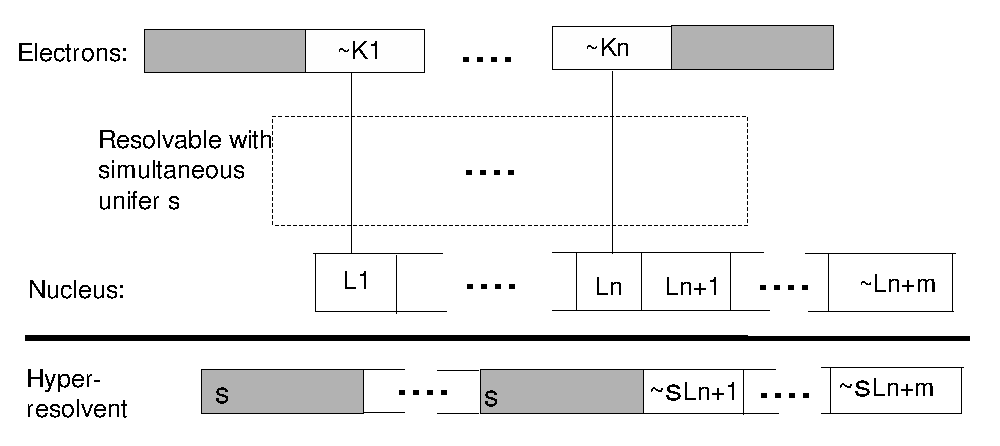
\includegraphics[width=\textwidth]{hyper-res.eps}
    \caption{hyper resolution �̃X�L�[��}
    \label{fig:hyper-res}
  \end{center}
\end{figure}

�}�� nucleus �Ƃ���̂�, ���Ȃ��Ƃ���‚̐��̃��e���������߂ł���.
�����”\�ȐߏW���ɂ͂��̂悤�Ȑ߂��K�����݂���.
nucleus �̌X�̐��̃��e�����ɂ‚�, ���̃��e�����݂̂����� electron ���K�v�ł���.
��͂�, �����”\�ȐߏW���ɂ͂��̂悤�Ȑ߂��K�����݂���.
nucleus �͑S�Ă� electron �Ɓu�����Ɂvresolve ����Ȃ���΂Ȃ�Ȃ�. 
���ʂƂ��ĕ��̃��e�����݂̂���Ȃ�߂�, ���o�߂Ƃ��ē�����(�}�� hyper-resolvent).
���̓��o�߂�, �ȍ~�� hyper-resolution �X�e�b�v�� electron �Ƃ��Ďg�p���邱�Ƃ��o����.

��X�̔����G���W���ł�, �t���O neg-hyper-res �� on �̎���
�g�p����� negative-hyper-resolution �ɑ�������.

\paragraph{Positive Hyper Resolution}

�t���O hyper-res �� on �̎��Ɏg�p�����̂�, ����� dual �Ȋ֌W�ɂ���,
\textsl{positive} hyper resolution �ł���. 
�����, ��ŏq�ׂ��X�L�[����, ���e������ ��/�� ���t�ɂ��鎖�œ����C
PI-resolution �ŁC���� $I$ �Ɋ܂܂��e���e�������ے�L�����܂ޏꍇ��
��������D

�ے�̌`�ŗ^�����錋�_��, �ʏ핉�̃��e�����݂̂��܂ނ��Ƃ���������,
negative hyper-resolution �� electron �Ƃ��ėp���鎖���o����̂�,
���_���牼��֌������Ă�, ��������_�ɓK���Ă���ƌ�����.
��� positive hyper-resolution ��, ���肩�猋�_�֌����Ă�, �O������
���_���”\�ł���. 

%%%%%%%%%%%%%%%%%%%%%%%%%%%%%
\subsection{Paramodulation}
\label{sec:paramod}

paramodulation �͓������������߂̐��_���[���ł���. 
�}~\ref{fig:paramod-rule} �� paramodulation �̃X�L�[��������.
�}��, $l = r$ �� \textbf{paramodulator} (���̓������e����), 
$f(t)$ �� $t$ �𕛍��Ɏ��‚悤�ȃ��e����
�ł���. $f(\sigma{r})$ ��, ���� $t$ �� $\sigma(r)$ �Œu������������
�\�����̂Ƃ���.

\begin{figure}[htbp]
  \begin{center}
    $$
    \infer{
      \begin{array}{ll}
        \mbox{\textbf{paramodulant:}} &
        f(\sigma r), \sigma L_1,\cdots,\sigma L_n,\sigma M_1,\cdots,\sigma M_m
      \end{array}
      }
    {\begin{array}{l}
        l = r, L_1,\cdots,L_n \\
        f(t), M_1,\cdots,M_m
      \end{array}\hskip2cm\sigma �� l �� t �� mgu
      }
    $$
    \caption{paramodulation �̃X�L�[��}
    \label{fig:paramod-rule}
  \end{center}
\end{figure}
�}��, $sigma$ ��, ���e���� $f(t)$ �̕��� $t$ �� paramdulator ��
���� $l$ �Ƃ� mgu(most general unifier) �ł��� ($\sigma l = t$).
paramodulant �� $t$ �� paramodulator �̉E�ӂ� $sigma$ ��K�p����
����($f(\sigma r)$) �Œu�������邱�Ƃɂ���ē�����.

%%%%%%%%%%%%%%%%%%%%%%%%%%%%%%%%%%%%%%%%%%%%%%%
\subsection{Demodulation}
\label{sec:demod}

demodulation �́C���o���ꂽ�߂ɓK�p����C����Ɋ܂܂�郊�e�����̃A�g����
�Ȗ񉻂���D
���Ȃ킿�C$l\rightarrow r$ �̌`������ demodulator ������C���郊�e����
$l$ ���� $t$ �𕛍��Ƃ��Ċ܂� $P[t]$ �̌`�����Ă�����̂Ƃ���D
���̂Ƃ��C$\sigma l = t$ �ƂȂ�悤�ȁC�ϐ��u�����������Ƃ��ɁC
$l$ ���C$P[\sigma r]$ �ɏ���������D

demodulator �Ƃ��āC$L = R$ �Ƃ��������̃��e�����݂̂���Ȃ�߂��p������D
������C���̏��������K���Ƃ��ėp���邽�߂ɂ́C
�����̕����t�����K�v�ł���D
�‚܂�C���炩�̏����֌W�ɂ���āC�����̍��E�ӂ�����t����K�v��
����D�����G���W���ł́C���̏����̔���ɁC�P���Ȏ��������� lrpo �� 2�� ��p�ӂ���D

\subsubsection{���s����demodulator����}
\label{sec:dynamic-demodulator}

�t���O dynamic-demod �� on �̏ꍇ, �����G���W����,
�S�Ă� equality ($\alpha = \beta$)�� demodulator �Ƃ��Ďg���邩
�ǂ����𔻒肷��.

�t���O dynamic-demod ���邢��, dynamic-demod-all �� on �ɂȂ��Ă���
�󋵂ł�, �K���t���O order-eq �� on �ɂȂ��Ă���͂��ł���.
���̎��t���O lrpo �� on �̏ꍇ�ɂ�, �����̌����‚��̔���Ƃ���
LRPO ��,
�����łȂ��ꍇ�͒P���ȏd�݂Ǝ��������ɂ���r���s����.
���̌��ʓ����̌����‚����s���邪, ����
�߂� demodulator �Ƃ��Ďg���邩�ǂ�����, ���̂悤�ȏ�����
���肳���.
�Ȃ������̑ΏۂƂ���߂�, ���� equality ���’P��߂ł���.

\begin{enumerate}
\item �߂̃��e���� $l (\alpha = beta)$ �Ɋւ��Ĉȉ��̔�������s����F
  \begin{description}
  \item[�t���O lrpo �� off �̏ꍇ]
    \begin{enumerate}
    \item $\beta$ �� $\alpha$ �̕����ł���� :normal �Ƃ���
    \item ���������̈Ӗ��� 
      $\alpha > \beta$ ���� $vars(\alpha) \supseteq vars(\beta)$
      �Ȃ��,
      \begin{enumerate}
      \item �t���O dynamic-demod-all �� on �ł���� OK �Ƃ���
      \item dynamic-demod-all �� off �� $wt(\beta)\leq 1$ �Ȃ��
        OK �Ƃ���
      \item ����ȊO�̏ꍇ�� NG �Ƃ���
      \end{enumerate}
    \item �t���O dynamic-demod-lex-dep �� dynamic-demod-all ��
      ������ on �̂Ƃ�, $\alpha$ �� $\beta$ ���ϐ������O�����,
      �\���I�ɓ���̍��ł���ꍇ�� ORDER-DEP �Ƃ���.
    \item ����ȊO�̏ꍇ�� NG �Ƃ���
    \end{enumerate}
  \item[�t���O lrpo �� on �̏ꍇ]
    \begin{enumerate}
    \item $l$ �̓����̌����‚����������s���Ă���ꍇ, OK �Ƃ���.
    \item �t���O dynamic-demod-lex-op �� on �̏ꍇ,
      $vars(\alpha)\supseteq vars(\beta)$ ORDER-DEP �Ƃ���.
    \item ����ȊO�̏ꍇ�� NG �Ƃ���
    \end{enumerate}
  \end{description}
\end{enumerate}

��̏�����, $vars(t)$ ��, �� $t$ �ɏo������ϐ��̏W�����Ӗ�����.

\subsubsection{Back Demdulation �̎��s}
\label{sec:back-demodulate}

back demodulation �Ƃ́C���o���ꂽ�߂����̒P��� equality ��
(��‚� $\alpha = \beta$ �̌`�̃��e�����݂̂���Ȃ��) ��
�������ꍇ�ɁC����� demodulator �Ƃ��ėp���āCusable �����
sos �Ɋ܂܂��S�Ă̐߂Ɋւ��� demodulation �����s������̂ł���D

���o�߂� demodulator �Ƃ��ēK�؂Ȃ��̂��ǂ����̔���́C
���o�߂ɑ΂���O����(��\ref{sec:pre-process}��
���Q��)�ōs���Ă���D

%%% Local Variables: 
%%% mode: latex
%%% TeX-master: t
%%% End: 


\newpage

% BIB %%%%%%%%%%%%%%%%%%%%%%%%%%%%%%%%%%%%%%%%%%%%%%%%%%%%%%
\begin{center}
\begin{thebibliography}{99}\itemsep=0pt

\bibitem{chang-lee} Chang, C. and Lee. R.C.,
  \textsl{Symbolic Logic and Mechanical Theorem Proving},
  Academic Press, 1973

\bibitem{ha} Joseph Goguen and Grant Malcolm, ``A Hidden Agenda'', in
  \emph{Theoretical Computer Science}, Vol.245 No.1, 2000, pp.55--101

\bibitem{otter} William McCune, ``\textsc{Otter3.0} Reference Manual
  and Guide'', Technical Report ANL-94/6, Argonne National Laboratory,
  1994, available at \texttt{http://www-unix.mcs.anl.gov/AR/otter/}

\bibitem{cafeobj} A.T.Nakagawa, T. Sawada, and K. Futatsugi,
  ``\textsl{CafeOBJ Manual}'', avaiable at 
  \texttt{ftp://ftp.sra.co.jp/lang/CafeOBJ/Manual/}

\bibitem{CafeRep} R\u{a}zvan Diaconescu and Kokichi Futatsugi,
  \textsf{CafeOBJ} \emph{Report}. World Scientific, 1998

\end{thebibliography}
\end{center}
\end{document}

